\def\OPTIONConf{0}
\def\OPTIONArxiv{0}
\documentclass[sigplan,review,anonymous]{acmart}\settopmatter{printfolios=true,printccs=false,printacmref=false}

\acmConference[PL'18]{ACM SIGPLAN Conference on Programming Languages}{January 01--03, 2018}{New York, NY, USA}
\acmYear{2018}
\acmISBN{} % \acmISBN{978-x-xxxx-xxxx-x/YY/MM}
\acmDOI{} % \acmDOI{10.1145/nnnnnnn.nnnnnnn}
\startPage{1}

\setcopyright{none}

\bibliographystyle{ACM-Reference-Format}

\usepackage{algorithm}
\usepackage[noend]{algpseudocode}
\usepackage{amsfonts}
\usepackage{amsmath}
\usepackage{amssymb}
\usepackage{amsthm}
\usepackage{boxedminipage}
\usepackage{color}
\usepackage{comment}
\usepackage{enumitem}
\usepackage{joshuadunfield}
\usepackage{lipsum}
\usepackage{mathpartir}
\usepackage{mathtools}
\usepackage{semantic}
\usepackage{slashed}
\usepackage{soul}
\usepackage{subcaption}
\usepackage[most]{tcolorbox}
\usepackage{upquote}
\usepackage{wrapfig}
\usepackage{xspace}

\makeatletter
\newcommand{\oset}[3][0ex]{%
  \mathrel{\mathop{#3}\limits^{
    \vbox to#1{\kern-0.75\ex@
    \hbox{$\scriptstyle#2$}\vss}}}}
\makeatother

\newcommand{\mc}[1]{\mathcal{{#1}}}
\newcommand{\todo}[1]{\emph{\hl{TODO:} {#1}}}
\newcommand{\saucy}{SaUCy\xspace}
\newcommand{\fstar}{$\text{F}^{\star}$}
\newcommand\myeq{\stackrel{\mathclap{\scriptsize\mbox{def}}}{=}}
\newcommand{\mypar}{\par}
\newcommand\doubleplus{+\kern-1.3ex+\kern0.8ex}
\newcommand{\yrightarrow}[1]{\xrightarrow{\raisebox{-2.5pt}[0pt][0pt]{#1}}}
\newcommand{\lollipop}[1]{\oset{{\rule{0ex}{0ex}\mkern-3mu{#1}}}{\lolli}}
\newcommand{\lollipopp}[1]{\oset{{\rule{0ex}{0ex}\mkern-3mu{#1}}}{\lolli}}
\newcommand*{\lolli}{%
  {\text{--}\mkern-2.4mu\text{---}\mkern-2.5mu\circ}% subformula acts as \mathord
}
\newcommand{\myheader}[1]{\noindent{\textit{\textbf{#1}}}}
\newcommand{\myheaderi}[1]{\textit{\textbf{#1}}}

% Functionality and ILC boxes
\newcommand{\Func}{\mc{F}}

\newtcolorbox{func}[1][]{title={\textbf{Functionality}~{#1}},enhanced,
  coltitle=black,
  top=0.2in,
  attach boxed title to top left=
  {xshift=0.5cm,yshift=-\tcboxedtitleheight/2},
  boxed title style={size=small, colback=white},colback=white}

\lstdefinestyle{myilc}
{
    language=Caml,
    keywordstyle={\bfseries},
    morekeywords={let, letrec, in, wr, rd, match, with},
    basicstyle={\sffamily},
    captionpos=b,
    columns=fullflexible,
    upquote = true,
    mathescape=true,
    showstringspaces=false,
}

\theoremstyle{definition}
\newtheorem{definition}{Definition}[section]

% ILC Expressions
\newcommand{\eVar}[1]{#1}
\newcommand{\eChan}[1]{#1}
\newcommand{\eUnit}{\Lparen\hspace{1px}\Rparen}
\newcommand{\ePair}[2]{\Lparen{#1},{#2}\Rparen}
\newcommand{\eInj}[2]{\keyword{inj}_{#1}\Lparen#2\Rparen}
\newcommand{\eRef}[1]{\keyword{ref}\Lparen{#1}\Rparen}
\newcommand{\eCase}[5]{\keyword{case}\Lparen{#1},{#2}.{#3},{#4}.{#5}\Rparen}
\newcommand{\eSplit}[4]{\keyword{split}\Lparen{#1},{#2}.{#3}.{#4}\Rparen}
\newcommand{\eGet}[1]{\keyword{get}\Lparen{#1}\Rparen}
\newcommand{\eSet}[2]{\keyword{set}\Lparen{#1},{#2}\Rparen}
\newcommand{\eFix}[2]{\keyword{fix}\Lparen{#1}.{#2}\Rparen}
\newcommand{\eLfix}[2]{\keyword{lfix}\Lparen{#1}.{#2}\Rparen}
\newcommand{\eLet}[3]{\keyword{let}\ {#1} = {#2}\ \keyword{in}\ {#3}}
\newcommand{\eLetRd}[4]{\eLet{\ePair{#1}{#2}}{\eRd{#3}}{{#4}}}
\newcommand{\eLetBang}[3]{\keyword{let!}\ {#1} = {#2}\ \keyword{in}\ {#3}}
\newcommand{\eBang}[1]{{!}\,{#1}}
\newcommand{\eLam}[2]{\lambda{#1}.\,{#2}}
\newcommand{\eLAM}[2]{\Lambda{#1}.\,{#2}}
\newcommand{\eApp}[2]{#1\,#2}
\newcommand{\eNu}[2]{\nu#1.\,#2}
\newcommand{\eWr}[2]{\keyword{wr}\Lparen{#1},{#2}\Rparen}
\newcommand{\eRd}[1]{\keyword{rd}\Lparen{#1}\Rparen}
\newcommand{\eFork}[2]{\ensuremath{#1 \xFork #2}}
\newcommand{\eChoice}[2]{\ensuremath{#1 \xChoice #2}}
\newcommand{\eSeq}[2]{{#1}\,;\,{#2}}

% ILC Types
\newcommand{\tyNat}{\tyname{nat}}
\newcommand{\tyBool}{\tyname{bool}}
\newcommand{\tyUnit}{\keyword{Unit}}
\newcommand{\tyProd}[2]{{#1} ** {#2}}
\newcommand{\tySum}[2]{{#1} + {#2}}
\newcommand{\tyRd}[1]{\keyword{Rd}\,#1}
\newcommand{\tyWr}[1]{\keyword{Wr}\,#1}
\newcommand{\tyRef}[1]{\keyword{Ref}\,#1}
\newcommand{\tyArr}[3]{{#1}\rightarrow_{#2}{#3}}
\newcommand{\emptyctxt}{\cdot}
\newcommand{\tyBang}[1]{{!}\,{#1}}
\newcommand{\tyTensor}[2]{{#1}\otimes{#2}}
%\newcommand{\tyLolli}[3]{{#1}\lollipop{#2}{#3}}
\newcommand{\tyLolli}[3]{{#1}\multimap_{#2}{#3}}

% ILC Modes
\newcommand{\Rm}{\textsf{R}}
\newcommand{\Wm}{\textsf{W}}
\newcommand{\Vm}{\textsf{V}}

% ILC Semantics
\newcommand{\Chans}{\Sigma}
\newcommand{\emptyChans}{\varepsilon}
\newcommand{\Store}{\sigma}
\newcommand{\Procs}{\pi}
\newcommand{\proc}[1]{#1}
\newcommand{\emptyProcs}{\varepsilon}
\newcommand{\Config}[3]{\left<#1;#2;#3\right>}

% ILC Misc
\newcommand{\xFork}{\mathrel{|\rhd}}
\newcommand{\xChoice}{\mathrel{\oplus}}
\newcommand{\e}{\epsilon}
\newcommand{\Lparen}{\textsf{(}}
\newcommand{\Rparen}{\textsf{)}}

%% Math ligatures (thanks to the semantic package) that make it
%% easier to typeset math using readable LaTeX text.
%\mathlig{|-->}{\longmapsto}
\mathlig{::=}{\bnfas}
\mathlig{:=}{\coloneqq}
\mathlig{|}{\;|\;}
% \mathlig{[[}{\mbsf{[}}
% \mathlig{]]}{\mbsf{]}}
\mathlig{[[}{\textsf{\upshape[}}
\mathlig{]]}{\textsf{\upshape]}}
\mathlig{**}{\times}
\mathlig{|>}{\rhd}
\mathlig{->}{\arr}
\mathlig{-->}{\rightarrow}
\mathlig{--->}{\longrightarrow}
\mathlig{=>}{\Rightarrow}
\mathlig{*!}{\boldsf{!}}
\mathlig{||}{\mathrel{|\!|}}
\mathlig{;;}{\mathrel{;}}
\mathlig{*&&}{\mathrel{\xFork}}
\mathlig{*||}{\mathrel{\oplus}}
\mathlig{!!}{\Downarrow}


% SaUCy specific
\newcommand{\msf}[1]{\ensuremath{{\mathsf {#1}}}}
\newcommand{\mtt}[1]{\ensuremath{\mathtt {#1}}}
\newcommand{\mcal}[1]{\ensuremath{\mathcal {#1}}}
\newcommand{\val}{\msf{val}}
\newcommand{\sn}{\msf{sn}}
\newcommand{\tn}{\textnormal}
\newcommand{\codeb}[1]{\textsf{#1}}
\newcommand{\hash}{\ensuremath{\mathcal{H}}}
\newcommand{\adv}{\ensuremath{{\mathcal A}}\xspace}
\newcommand{\Adv}{\adv}
\newcommand{\A}{\adv}
\newcommand{\samples}{\overset{\$}{\leftarrow}}
\newcommand{\SA}{\msf{SA}}
\newcommand{\SaUCy}{\xspace{\msf{SaUCy}}\xspace}
\newcommand{\leak}{\color{blue}\mtt{leak}}
\newcommand{\eventually}[1]{\color{blue}\mtt{leak}}
\newcommand{\poly}{\textnormal{poly}}
\newcommand{\negl}{\textnormal{negl}}
\newcommand{\execUC}[4]{\mathsf{execUC}({#1},{#2},{#3},{#4})}
\newcommand{\chan}[1]{{\underline{\smash{\msf{#1}}}}}
\newcommand{\functionality}[1]{\ensuremath{\mathcal{F}_{\textnormal{\msf{{#1}}}}}}
\newcommand{\F}{\functionality}
%\newcommand{\G}[1]{\mathcal{G}_{\textnormal{\tiny {\uppercase{#1}}}}}
\newcommand{\GG}[1]{{\overline \mathcal{G}}_{\textnormal{\tiny {\uppercase{#1}}}}}
\renewcommand{\C}[1]{\mathcal{C}_{\textnormal{\tiny {\uppercase{#1}}}}}
\renewcommand{\P}{\ensuremath{\mathcal P}}
\newcommand{\Ps}{\ensuremath{\{\mathcal{P}_i\}_{i \in [N]}}}
\renewcommand{\S}{\ensuremath{\mathcal S}}
\newcommand{\env}{\Z}
\newcommand{\Z}{{\mcal{E}}}
\newcommand{\R}{{\mathcal R}}


\begin{document}

\title[SaUCy]{A Calculus for Composable Cryptography}

\author{Kevin Liao}
\affiliation{
  \institution{University of Illinois Urbana-Champaign}
}
\email{kliao6@illinois.edu}

\author{Matthew Hammer}
\affiliation{
  \institution{University of Colorado Boulder}
}
\email{matthew.hammer@colorado.edu}

\author{Andrew Miller}
\affiliation{
  \institution{University of Illinois Urbana-Champaign}
}
\email{soc1024@illinois.edu}

\begin{abstract}
  The universal composability (UC) framework is the established standard for
  analyzing cryptographic protocols in a modular way, such that security is
  preserved under concurrent composition with arbitrary other protocols.
  However, although UC is widely used for on-paper proofs, prior attempts at
  systemizing it have fallen short, either by using a symbolic model (thereby
  ruling out computational reduction proofs), or by limiting its expressiveness.

  In this paper, we lay the groundwork for building a concrete, executable
  implementation of the UC framework. Our main contribution is a process
  calculus, dubbed the Interactive Lambda Calculus (ILC). ILC faithfully
  captures the computational model underlying UC---interactive Turing machines
  (ITMs)---by adapting ITMs to a subset of the $\pi$-calculus through an affine
  typing discipline. In other words, \emph{well-typed ILC programs are
    expressible as ITMs.} In turn, ILC's strong confluence property enables
  reasoning about cryptographic security reductions.  We use ILC to develop a
  simplified implementation of UC called SaUCy.
\end{abstract}


\maketitle

\section{Introduction}
\label{sec:introduction}

\begin{comment}
The success of blockchains and cryptocurrencies have raised interest in building
secure software systems that combine consensus protocols~\cite{miller2016honey},
zero-knowledge proofs~\cite{kosba2016hawk}, multiparty
computation~\cite{bentov2017instantaneous}, and other advanced techniques from
distributed computing and cryptography.  However, these primitives are known to
be error-prone and difficult to compose securely.  To the average developer,
reasoning about asynchronous, distributed, and adversarial deployment
environments is unnatural. On top of this, the security of a software system is
generally a whole-system property, but vulnerabilities often arise from
misunderstandings and mismatches as components are
integrated~\cite{chong2016report}.

Our solution is to develop a module system, \saucy, that will simplify the task
of composing distributed protocols and cryptographic primitives.  The novel
design idea of \saucy is to include with each module a rich behavioral
specification in the form of an \emph{ideal functionality}, which serves as a
self-contained specification of all desired security and liveness properties.
This idea is rooted in the theory of \emph{universal composability}
(UC)~\cite{canetti2001universally}, which is widely used in cryptography for
on-paper proofs, but has not yet been adapted for software engineering.  Based
on our prior experience providing formal specifications for smart contract and
blockchain protocols~\cite{bentov2017instantaneous, kosba2016hawk,
  miller2017sprites}, ideal functionalities are well-suited for modular design
of complex security-oriented applications for several reasons:

\begin{enumerate}
\item The UC framework is an established standard for modeling distributed and
  cryptographic protocols, so we can draw on existing literature for ideal
  functionality models.
\item Ideal functionalities are executable specifications, so they are amenable
  to property-based testing and machine-checkable proofs.
\item UC provides the strongest notion of security under concurrent
  composition. When we substitute an ideal functionality for a distributed
  protocol that realizes it, all the properties of the ideal functionality are
  preserved. Hence a developer's understanding of the ideal functionality
  carries over to the distributed implementation.
\end{enumerate}

\subsection{Our Approach}
\label{subsec:approach}

To reap the expected benefits of the \saucy module system, in this work, we will
develop infrastructure to help authors write, test, and verify distributed
protocol and cryptographic primitives.  This work will take place over three
main tasks: The first task focuses on designing a new high-level language called
ILC for expressing protocols and implementing the UC framework, the second
task focuses on developing testing techniques for detecting security and
liveness violations in the presence of Byzantine failures, and the third task
focuses on building a verification tool for mechanizing security and liveness
proofs in the UC framework.\smallskip

\subsection{Organization}
\label{subsec:org}

This paper is organized as follows. Section~\ref{sec:background} provides an
overview of the UC framework and potential applications.
Section~\ref{sec:challenges} highlights several challenges in using
UC. Section~\ref{sec:ilc} describes the design of our programming language
Interactive Lambda Calculus (ILC). Section~\ref{sec:session} describes an
extension of ILC with session types that will enable a form of verification for
ILC programs. Section~\ref{sec:testing} details our plan to develop new
techniques for testing security and liveness of ILC procotols in the presence of
Byzantine failures. Section~\ref{sec:verification} details our plan to develop a
proof assistant for mechanizing UC proofs.
\end{comment}


\section{Overview of ILC and SaUCy}
\label{sec:background}

We tour the universal composability framework and give a flavor of ILC and SaUCy
with the simple example of how two untrusting parties, Alice and Bob, can
securely flip a coin using a commitment scheme.

\begin{figure*}[t]
\centering
\begin{tabular}{c|c}
\begin{subfigure}{.575\textwidth}
    $\Func_{\textsc{com}}$ proceeds as follows, running with parties $A$ and
  $B$.
    \begin{enumerate}
        \item Upon receiving a message $(\mathsf{Commit}, b)$ from $A$, where $b
          \in \{ 0, 1 \}$, record the value $b$ and send the message
          $(\mathsf{Receipt})$ to $B$. Ignore any subsequent \textsf{Commit}
          messages.
        \item Upon receiving a message $(\mathsf{Open})$ from $A$, proceed as
          follows: If some value $b$ was previously recorded, then send the
          message $(\mathsf{Open}, b)$ to $B$ and halt. Otherwise, halt.
    \end{enumerate}
\label{func:com}
\end{subfigure}\hspace{0.02\textwidth}
&\hspace{0.02\textwidth}
\begin{subfigure}{.35\textwidth}
  \lstinputlisting[style=myilc]{listings/Fcom.ilc}
\end{subfigure}
\end{tabular}
\caption{An ideal functionality for a one-time commitment scheme in prose (left)
  and in ILC (right).}
\label{func:com}
\end{figure*}

\subsection{Ideal Functionalities}
\label{subsec:functionalities}

Security in the UC framework is based on the real/ideal
paradigm~\cite{goldreich1987play}. To carry out some cryptographic task in the
real world, a set of parties must execute a protocol for the task among
themselves in a distributed fashion. In the ideal world, however, the parties
securely access an \emph{ideal functionality} $\mc{F}$, which is imagined as an
incorruptible trusted third party that securely (by construction) carries out
the task to be achieved by the protocol. The idea is that $\mc{F}$ obtains
inputs from the parties, carries out the task locally, and returns outputs back
to the parties. This serves as a self-contained specification
for the task's security requirements.\smallskip

\myheader{Example: Secure coin flipping.} Suppose two untrusting parties, Alice
and Bob, wish to securely flip a coin---Alice calls the coin flip by publishing $b
\in \{ 0, 1\}$, and Bob flips the coin by publishing $r \in \{0, 1\}$. If $b = r$,
then Alice wins; otherwise, Bob wins. Observe that simply having Alice and Bob
publish their respective values is not secure. If Alice publishes $b$ first,
then Bob can cheat by manipulating $r$ in his favor (and vice versa)!

In order to carry out the coin flip securely, they can use a commitment
scheme~\cite{brassard1988minimum}. Alice first publishes a commitment $C =
\mathsf{com}(b)$ for her bit $b$, waits for Bob to publish $r$, and then opens
and publishes a bit $b' = \mathsf{open}(C)$. If $r = b'$, then Alice wins;
otherwise, Bob wins.  Now, in order for such a commitment scheme to be secure,
it should satisfy the \emph{hiding} property (i.e., $C$ hides $b$ from Bob, so
he cannot manipulate $r$ in his favor) and the \emph{binding} property (i.e.,
$b=b'$, so that Alice cannot change the committed value in her favor).\smallskip

\myheader{Commitment functionality.} We can capture both of these properties at
once by defining an ideal functionality $\Func_{\textsc{com}}$ for a (one-time)
commitment scheme as it would appear in the cryptography literature
(Figure~\ref{func:com}, left). Upon receiving the bit $b$ that Alice commits to,
$\Func_{\textsc{com}}$ records $b$ and notifies Bob that it has done so. Then,
whenever Alice wants to reveal $b$ to Bob, she notifies $\Func_{\textsc{com}}$,
which sends it to Bob. Because, in this idealized world, Alice and Bob trust
$\Func_{\textsc{com}}$ to do all the work, the hiding and binding properties
hold trivially. Of course, in the real world, Alice and Bob would not want to
trust such a third party (if it even exists), so their hope is that the
commitment scheme they use is ``just as good as''
$\Func_{\textsc{com}}$.\smallskip

\subsection{A Flavor of ILC}
\label{subsec:ilc-flavored}

In Figure~\ref{func:com} (right), we have written $\Func_{\textsc{com}}$ in
ILC. The function \textsf{fCom} takes as arguments a read channel \textsf{frA},
which receives messages from $A$, and a write channel \textsf{toB}, which sends
messages to $B$. In ILC, channels are typed, so each of these channels
communicates values inhabiting the sum type \textsf{Msg}. Moreover, read
channels are linearly typed so that they are protected from duplication. This
ensures that no confusion arises as to which process is being written to. On the
other hand, write channels are intuitionistically typed, so their use is
unrestricted.

Because \textsf{fCom} consumes a linear read channel, its type signature
consists of linear arrows $\multimap$ (or ``lollipops''), which describe the types
of linear functions that consume their arguments exactly once. But what if we
want a linear function to operate over unrestricted values? In that case, the !
operator (pronounced ``bang!'') permits an intuitionistically typed value to be
used in an unrestricted manner as a linearly typed value, i.e., contraction or
weakening may be used. This explains why the type of \textsf{frA} is \textsf{Rd
  Msg} and the type of \textsf{toB} is \textsf{!(Wr Msg)}.

An ILC expression is also typed with a mode $m \in \{\Wm, \Rm, \Vm\}$, denoting
the write, read, and value modes, respectively. Arrow types, both linear and
intuitionistic, carry the mode of their function bodies, so in the function
signature of \textsf{fCom}, the left lollipop implicitly carries a mode $\Vm$,
which we have chosen to elide, and the right lollipop carries a mode $\Rm$,
which is the mode of its body.

The function body of \textsf{fCom} closely follows $\Func_{\textsc{com}}$, but
several points are worth mentioning.  First, we introduce the typing rules of
expressions for reading and writing on a channel. Recall that typing judgements
have the form $\Delta ; \Gamma |- e : A |> m$, where $\Delta$ is a linear typing context, $\Gamma$
is an intuitionistic typing context, and $m$ is a mode.
\begin{mathpar}
\Infer{letrd}
{\Delta_1 ; \Gamma |- e_1 : \tyRd{A}\\
\Delta_2,x_1:\tyBang{A},x_2:\tyRd{A} ; \Gamma |- e_2 : B |> m
}
{\Delta_1, \Delta_2 ; \Gamma |- \eLetRd{x_1}{x_2}{e_1}{e_2} : B |> \Rm}
\end{mathpar}

The letrd rule says that if we can partition the linear context $\Delta$ as $\Delta_1,
\Delta_2$ such that $e_1$ has type $\tyRd{A}$ and mode $\Vm$ (elided) under contexts
$\Delta_1; \Gamma$ and $e_2$ has type $B$ and mode $m$ under contexts
$\Delta_2,x_1:\tyBang{A},x_2:\tyRd{A} ; \Gamma$, then the full expression has type $B$ and
mode $\Rm$. Here, the idea is that reading a channel of type $\tyRd{A}$ gives a
linear pair (or ``tensor'') of type $\tyTensor{\tyBang{A}}{\tyRd{A}}$. Because
ILC only allows intuitionistically typed values to be sent over channels, the
intuitionistic value read from the channel is lifted into the first element of
the tensor as a linear type. The second element rebinds the read channel, so
that it may be used again.  In \textsf{fCom}, pattern matching with the !
operator unpacks linear values of type $\tyBang{A}$, so the value bound to $b$
in the first read from \textsf{frA} has an intuitionistic type.
\begin{mathpar}
\Infer{wr}
{\Delta_1; \Gamma   |- e_1 : A\\
\Delta_2; \Gamma   |- e_2 : \tyWr{A}}
{\Delta_1, \Delta_2; \Gamma |- \eWr{e_1}{e_2} : \tyUnit |> \Wm}
\end{mathpar}

The wr rule says that if we can partition the linear context $\Delta$ as $\Delta_1, \Delta_2$
such that $e_1$ has type $A$ and mode $\Vm$ and $e_2$ has a type $\tyWr{A}$ and
mode $\Vm$, then the full expression has type $\tyUnit$ and mode $\Wm$.

What is not showcased in these two rules is mode composition. In ILC, modes can
be composed in two ways: sequentially (i.e., $m ;; n => p$) and in parallel
(i.e., $m || n => p$). The rules for mode composition, which we describe in full
in Section~\ref{sec:ilc}, disallow the parallel composition of two write mode
processes. That is, $\Wm || \Wm => p$ is not derivable for any mode $p$. This
ensures that no confusion arises as to which process is writing (i.e., is
activated), since in the ITM model only a single process is active at any given
time. In \textsf{fCom}, each of the letrd expressions is read mode, and
sequentially composing two read mode expressions yields a read mode expression
(i.e., $\Rm ;; \Rm => \Rm$ according to our mode composition rules). As
aforementioned, the right lollipop in \textsf{fCom}'s type signature carries the
mode $\Rm$.

\subsection{UC Emulation}
\label{subsec:emulation}

Having defined security in the form of an ideal functionality, the next step is
to prove that a protocol meets the definition. We say that a protocol $\pi$
\emph{emulates} (or \emph{securely realizes}) an ideal functionality $\mc{F}$ if
every adversarial behavior in the real world (running with $\pi$) can also be
exhibited in the ideal world (running with $\mc{F}$). But because $\mc{F}$ is
secure by construction, whatever adversarial behavior can take place in the
ideal world does not lead to a break in security.

Proving emulation formally proceeds in two steps. The first step is
constructive: We must construct a \emph{simulator} $\mc{S}$ (a simulated
adversary) that can emulate the attack of any adversary $\mc{A}$ on $\pi$, but
instead, on $\mc{F}$. The second step is a relational analysis: We must show
that running $\pi$ under attack by any adversary $\mc{A}$ (the real world) is
\emph{indistinguishable} from running $\mc{F}$ under attack by $\mc{S}$ (the
ideal world) to any distinguisher $\mc{Z}$, called the \emph{environment}. In
particular, $\mc{Z}$ is an interactive distinguisher: It interacts with the real
world and the ideal world in a well-defined manner, and the simulation is good
if no $\mc{Z}$ can distinguish between the two.

\begin{figure}
  \centering
  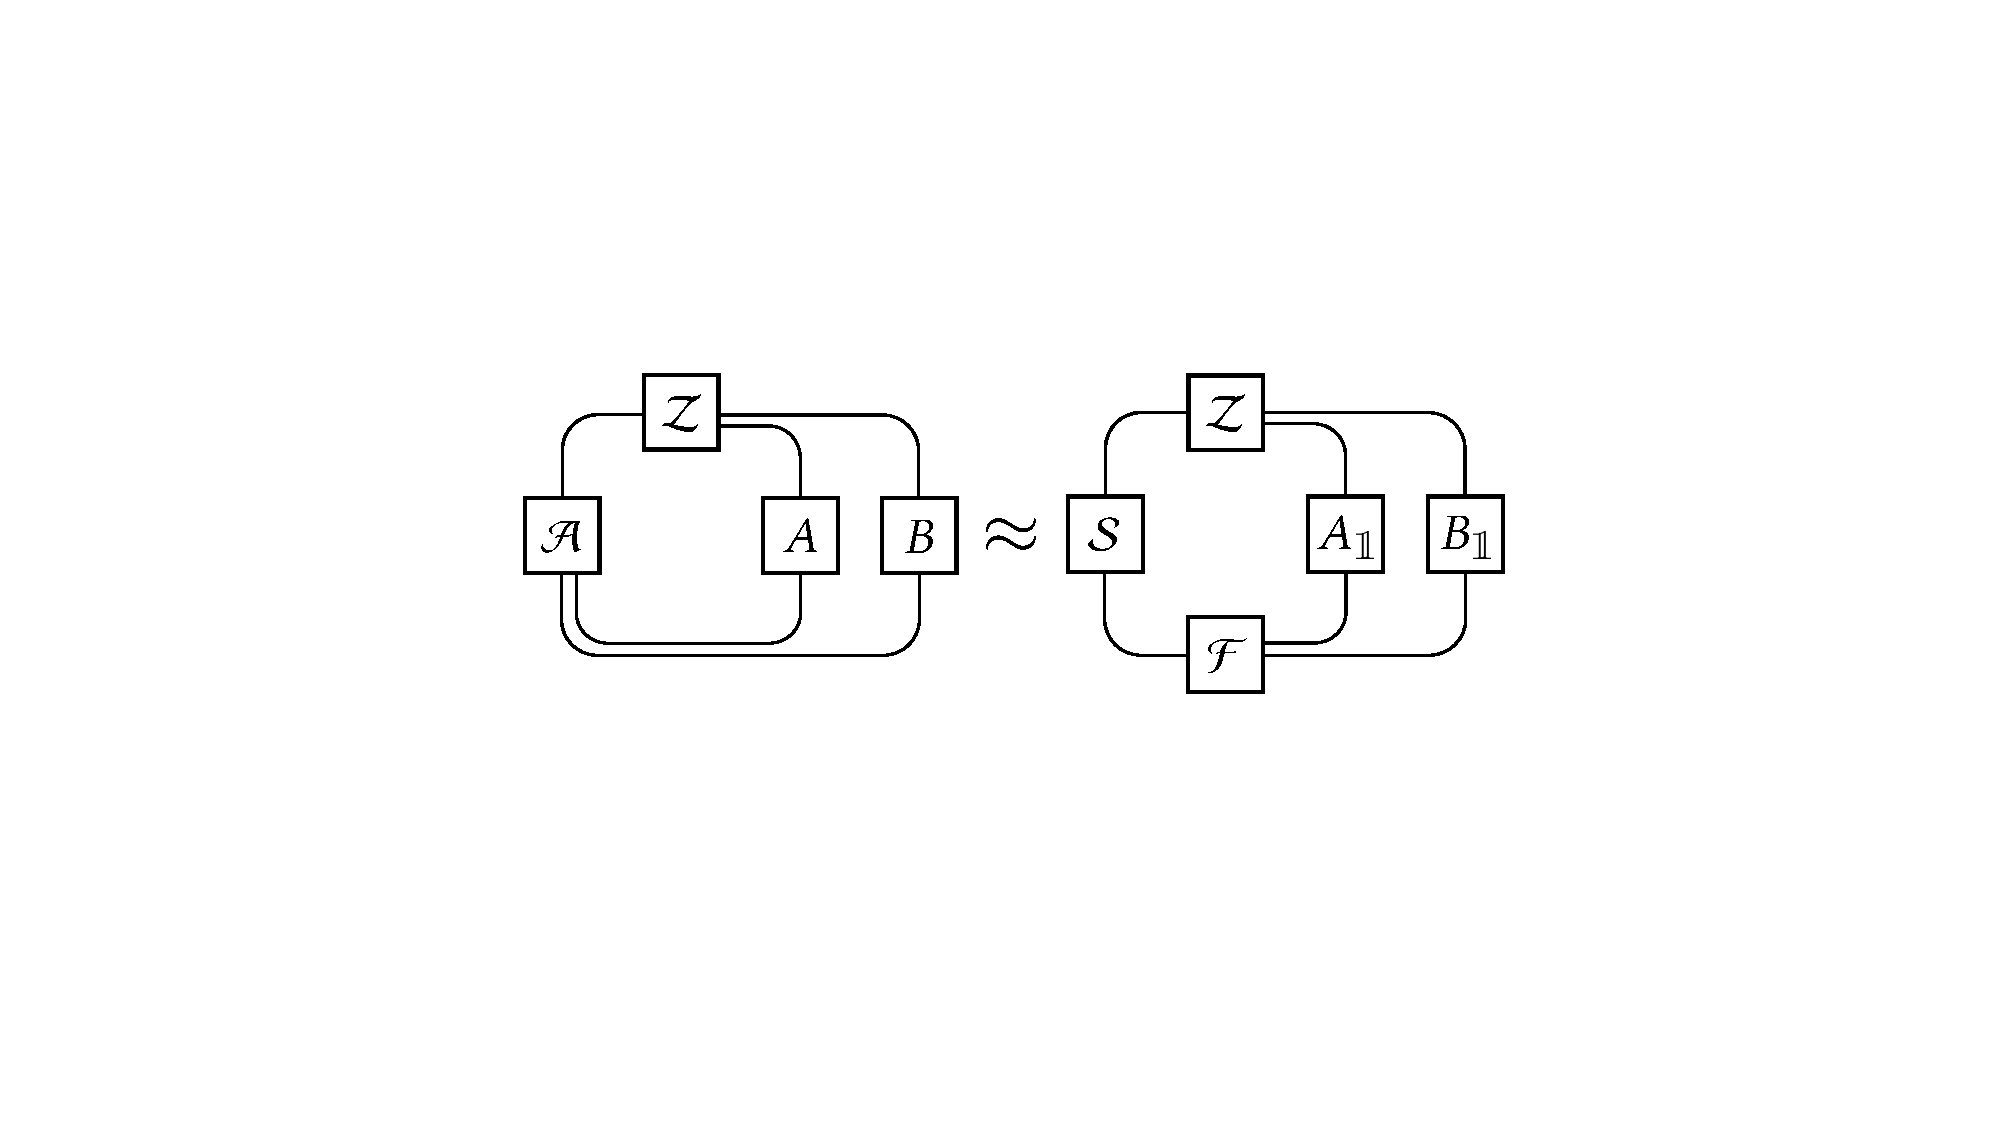
\includegraphics[width=0.85\linewidth]{graphics/suc-experiment}
  \caption{UC experiment with real world (left) and ideal world (right).}
  \label{fig:uc-experiment}
\end{figure}

Figure~\ref{fig:uc-experiment} illustrates the UC experiment in the context of
the commitment scheme we defined before. The real world is shown on the left and
the ideal world is shown on the right, with connecting lines denoting
communication channels.\footnote{Note that in the real world, all communication
  passes through the adversary $\mc{A}$. In the bare model, communication is
  asynchronous, unauthenticated, and unreliable, but other models of
  communication can be built atop this model.} In the real world, $A$ and $B$
carry out the protocol with eachother, while in the ideal world, $A$ and $B$ are
``dummy'' parties that simply relay messages between $\mc{Z}$ and $\mc{F}$. The
environment $\mc{Z}$ is tasked to interact with each world and distinguish
between the two.

\subsection{A Flavor of SaUCy}
\label{subsec:sauce-flavored}

\todo{SaUCy concrete implementation and prelude, UC metatheory}



\begin{comment}
\subsection{UC composition}
\label{subsec:composition}

The advantage of security definitions in UC is that they satisfy strong
composability guarantees, even under concurrent composition. Suppose that $\pi_1$
is a protocol that securely realizes a functionality $\mc{F}_1$. If a protocol
$\pi_2$, using $\mc{F}_1$ as a subroutine, securely realizes a functionality
$\mc{F}_2$, then the protocol $[\pi_1 / \mc{F}_1]\pi_2$, in which calls to
$\mc{F}_1$ are replaced by calls to $\pi_1$, also securely realizes
$\mc{F}_2$. That way, it suffices to analyze the security of the standalone
protocol $\pi_2$ in the $\mc{F}_1$-hybrid model, where parties run $\pi_2$ with
access to $\mc{F}_1$, as opposed to the composite protocol of $\pi_2$ and
$\pi_1$. Figure~\ref{fig:uc-composition} illustrates protocol composition. The
setup on the left represents the $\mc{F}_1$-hybrid model, and the setup on the
right represents the protocol substitution $[\pi_1 / \mc{F}_1]\pi_2$, which
maintains security.

\begin{figure}
  \centering
  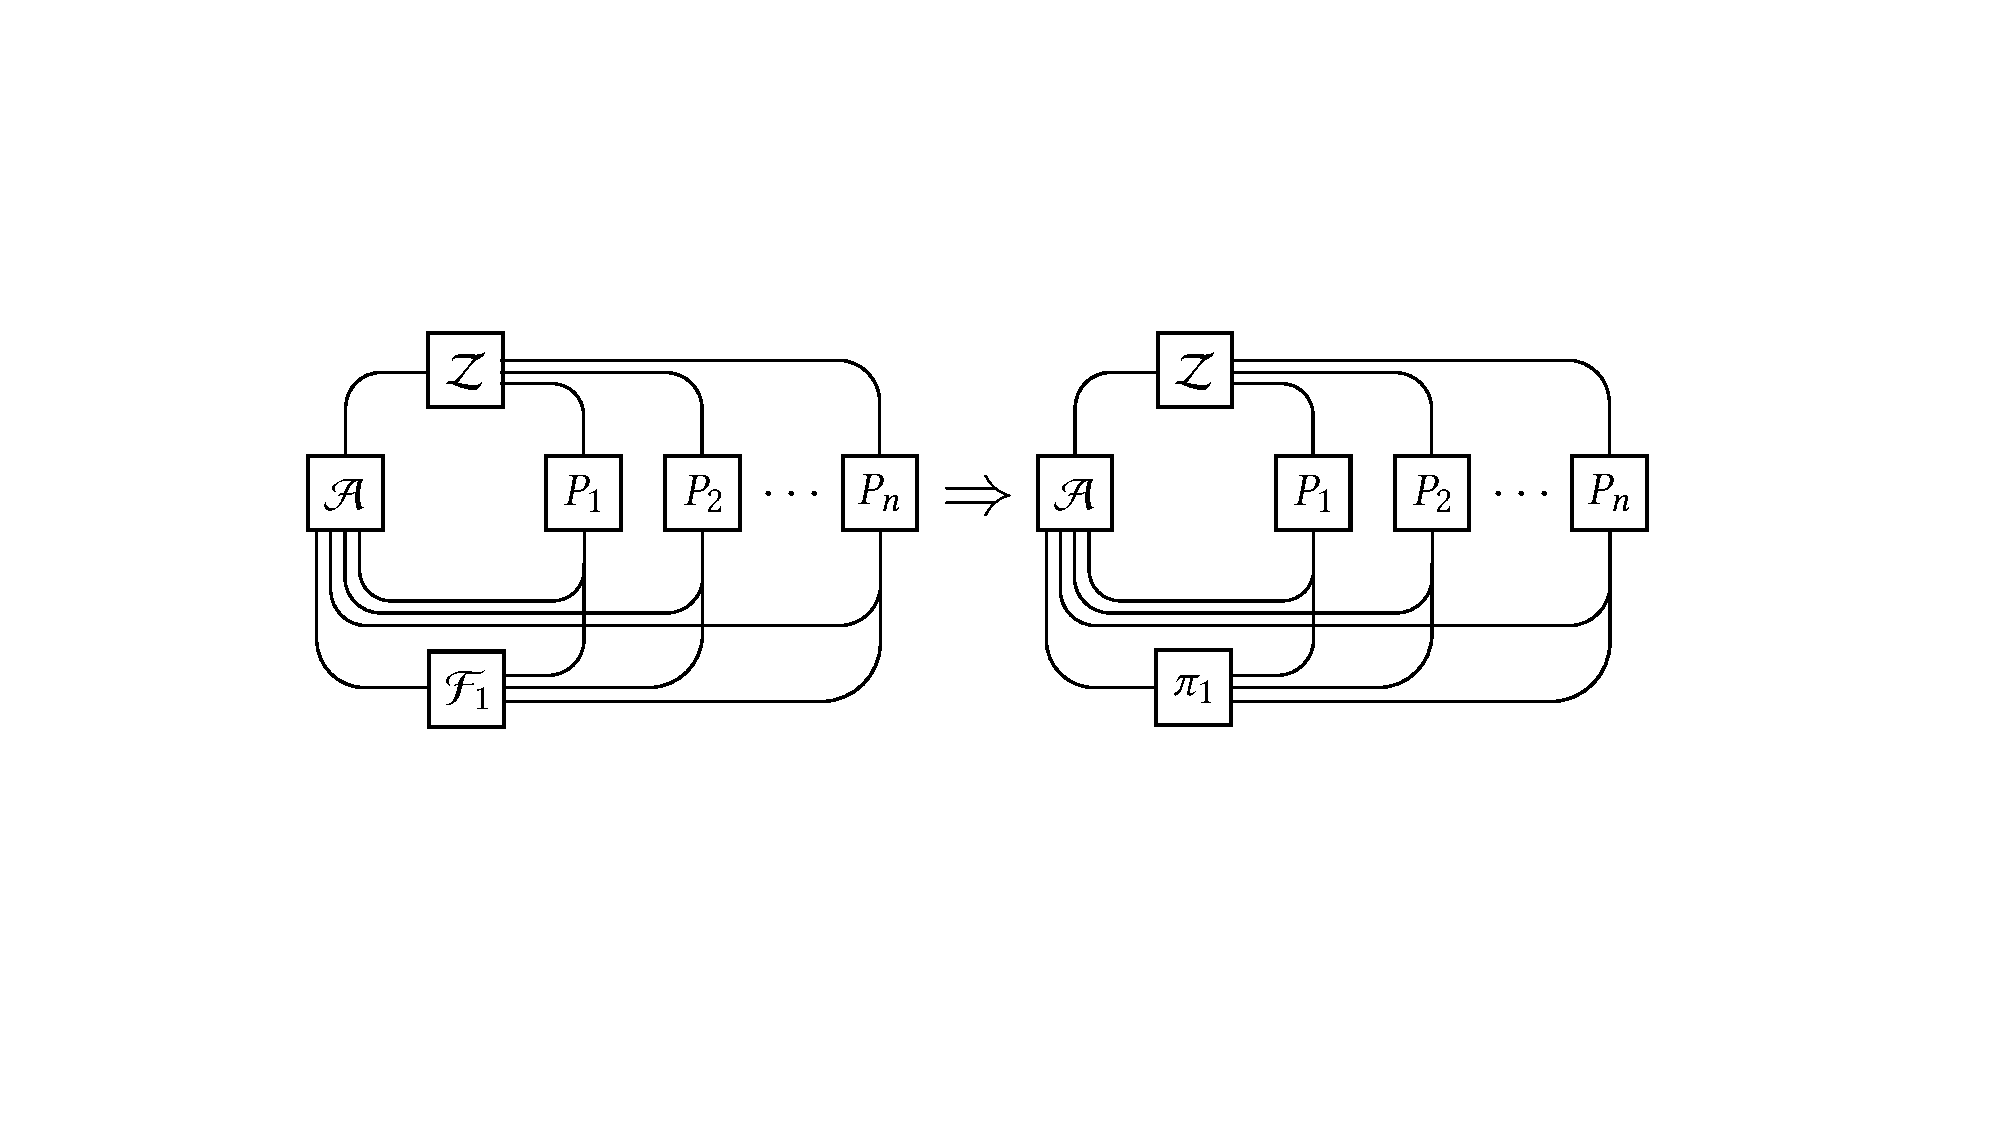
\includegraphics[width=\linewidth]{graphics/composition}
  \caption{UC protocol composition theorem.}
  \label{fig:uc-composition}
\end{figure}
\end{comment}


\section{Interactive Lambda Calculus}
\label{sec:ilc}

Adapting theory from UC into a concrete implementation turns out to be
difficult. To begin with, the computational model underlying UC, called
Interacting Turing Machines (ITMs), is not a good fit to existing distributed
languages. In the ITM model, execution is essentially single threaded, passing
control from one process to another each time a message is sent, such that
exactly one process is active at a given time. This is in contrast to the
standard $\pi$-calculus~\cite{milner1999communicating}, for which there may be
many possible execution paths that lead to different outcomes.

Therefore, we have developed a core process calculus, called Interactive Lambda
Calculus (ILC), that adapts ITMs to a subset of the $\pi$-calculus through its
type system. In particular, the invariants maintained by the type system ensures
that any non-determinism is due to random coinflips taken by processes, which
have a well-defined distribution. This is essential to ensure that the
normalization of an ILC program has a computational interpretation, as is
necessary in cryptographic reduction proofs.

Using ILC, we will implement the UC network model (asynchronous communication,
Byzantine corruptions, etc.) and executable UC implementations (ideal
functionalities and simulators) for various primitives in the distributed
systems and cryptography literature (e.g., distributed consensus, multiparty
computation, and zero-knowledge proofs).

\subsection{Program Syntax}
\label{subsec:syntax}

Figure~\ref{fig:ilc-syntax} gives the syntax of expressions. Expressions $e$
include variables $x$, primitive values $v$, channels $c$, the unit value $()$,
pairs (with elimination form \textsf{split}), sums (with elimination form
\textsf{case}), reference cells (with elimination form \textsf{get} and mutable
update \textsf{set}), thunks (with elimination form \textsf{force}), fixed
points, let binding, lambda abstraction, and function application. For
communication, expressions include restriction ($\eNu{(x_1, x_2)}{e}$), which
binds a a read channel $x_1$ and write channel $x_2$ in $e$; send
($\eWr{e_1}{e_2}$), which writes the result of evaluating $e_1$ on the channel
result of evaluating $e_2$; receive ($\eRd{e}$), which reads from the channel
result of evaluating $e$ and returns a pair consisting of the read value and the
read channel itself (see Section~\ref{subsec:types} for details); fork ($e_1 *&&
e_2$), which creates a separate process $e_1$ and continues as $e_2$; external
choice ($e_1 *|| e_2$), which allows a process to evolve as either $e_1$ or
$e_2$ (based on some initial event in each of the processes); and sequential
composition ($e_1 ; e_2$).

\begingroup
\setlength\intextsep{0pt}
\begin{wrapfigure}{r}{0.35\textwidth}
  \lstinputlisting[style=myilc]{listings/loop.ilc}
\end{wrapfigure}
Note that replication ($!e$ in the $\pi$-calculus), which allows a process to
spawn repeatedly, is not included for reasons we discuss in
Section~\ref{subsec:types}. Instead, replication can be achieved through
recursive definitions. For example, the recursive function \textsf{loop} (right)
takes as arguments a read channel \textsf{c} and a function \textsf{f}. In the
definition of \textsf{loop}, the let expression binds the value read from
\textsf{c} to the variable \textsf{v} and rebinds the read channel to
\textsf{c}; the body of the let expression applies the function \textsf{f} to
the value \textsf{v}, and then repeats \textsf{loop}.\mypar
\endgroup

\begin{figure*}
  \begin{grammar}
    Expressions
    & $e$
        &$\bnfas$&
        $\eVar{x} \bnfalt \eUnit \bnfalt \ePair{e_1}{e_2} \bnfalt \eInj{i}{e}
    \bnfalt \eRef{e} \bnfalt \eSplit{e_1}{x_1}{x_2}{e_2} \bnfalt
    \eCase{e}{x_1}{e_1}{x_2}{e_2}$
    \\ &&& $\bnfaltbrk \eGet{e} \bnfalt \eSet{e_1}{e_2} \bnfalt \eFix{x}{e}
    \bnfalt \eLet{x}{e_1}{e_2} \bnfalt \eLetBang{x}{e_1}{e_2} \bnfalt \eBang{e}$
    \\ &&& $\bnfaltbrk \eLam{x}{e} \bnfalt \eApp{e_1}{e_2} \bnfalt \eNu{(x_1,
      x_2)}{e} \bnfalt \eWr{e_1}{e_2} \bnfalt \eLetRd{x_1}{x_2}{e_1}{e_2}$
    \\ &&& $\bnfaltbrk \eFork{e_1}{e_2} \bnfalt \eChoice{e_1}{e_2} \bnfalt
    \eSeq{e_1}{e_2}$
  \end{grammar}
  \caption{Syntax of expressions.}
  \label{fig:ilc-syntax}
\end{figure*}


\subsection{Type System}
\label{subsec:types}

\begin{figure*}
  \begin{grammar}
    Types
    & $A,B$
    &$\bnfas$& $\tyUnit \bnfalt \tyProd{A}{B} \bnfalt \tySum{A}{B} \bnfalt \tyRd{A} \bnfalt
    \tyWr{A} \bnfalt \tyRef{A} \bnfalt \tyArr{A}{\footnotesize $m$}{B}$
    \\
    Linear Typing Contexts
    & $\Delta$
    &$\bnfas$& $\emptyctxt \bnfalt \Delta,x:A$
    \\
    Intuitionistic Typing Contexts
    & $\Gamma$
    &$\bnfas$& $\emptyctxt \bnfalt \Gamma,x:A$
  \end{grammar}
\caption{Syntax of types.}
\label{fig:syntax--types}
\end{figure*}


\begin{figure*}[htbp]
  \centering
  \begin{grammar}
    Modes & $m,n,p$ &$\bnfas$& $\Wm \bnfalt \Rm \bnfalt \Vm$
  \end{grammar}

  \judgbox{m || n => p}{~~The parallel composition of modes $m$ and $n$ is mode~$p$.}
  \begin{mathpar}
  \Infer{sym}{m || n => p}{n || m => p}
  \and \Infer{wv}{ }{\Wm || \Vm => \Wm}
  \and \Infer{wr}{ }{\Wm || \Rm => \Wm}
  \and \Infer{rv}{ }{\Rm || \Vm => \Rm}
  \and \Infer{rr}{ }{\Rm || \Rm => \Rm}
  \and \Infer{vv}{ }{\Vm || \Vm => \Vm}
  \end{mathpar}
  \\[2mm]
  \judgbox{m ;; n => p}{~~The sequential composition of modes $m$ and $n$ is mode~$p$.}
  \begin{mathpar}
  \Infer{w*}{ }{\Wm ;; n => n}
  \and \Infer{r$\ast$}{ }{\Rm ;; n => \Rm}
  \and \Infer{v$\ast$}{ }{\Vm ;; n => n}
  \end{mathpar}
  \\[2mm]
  \judgbox{m || n\ \slashed{=>}\ p}{~~The parallel composition of modes $m$ and $n$ is
    \emph{not derivable} for any mode~$p$.}
  \begin{mathpar}
  \Infer{ }{ }{\Wm || \Wm\ \slashed{=>}\ p}
  \end{mathpar}
\caption{Syntax of modes; sequential and parallel mode composition.}
\label{fig:syntax-modes}
\end{figure*}


\begin{figure*}[htbp]
\centering
\judgbox{\Delta ; \Gamma |- e : A |> m}{~~Under $\Delta$ and $\Gamma$, expression~$e$ has
  intuitionistic type $A$ and mode $m$.}
\begin{mathpar}
\Infer{var}
{\Gamma(x) = A}
{\Delta; \Gamma |- x: A}
%
\and
%
\Infer{unit}
{ }
{\Delta ; \Gamma |- \eUnit : \tyUnit}
%
\and
%
\Infer{pair}
{\Delta_1; \Gamma |- e_1 : A_1\\\\
\Delta_2; \Gamma |- e_2 : A_2}
{\Delta_1, \Delta_2; \Gamma |- \ePair{e_1}{e_2} : \tyProd{A_1}{A_2}}
%
\and
%
\Infer{inj}
{i \in \{1, 2\}\\\\
\Delta; \Gamma |- e : A_i}
{\Delta ; \Gamma |- \eInj{i}{e}  : \tySum{A_1}{A_2}}
%
\and
%
\Infer{ref}
{\Delta; \Gamma |- e : A}
{\Delta; \Gamma |- \eRef{e} : \tyRef{A}}
%
\and
%
\Infer{split}
{\Delta_1; \Gamma |- e_1 : A_1 \times A_2\\\\
\Delta_2; \Gamma,x_1:A_1, x_2:A_2 |- e_2 : B |> m}
{\Delta_1, \Delta_2; \Gamma |- \eSplit{e_1}{x_1}{x_2}{e_2} : B |> m}
%
\and
%
\Infer{case}
{\Delta_1; \Gamma |- e : A_1 + A_2\\\\
\Delta_2; \Gamma,x_1:A_1 |- e_1 : B |> m\\\\
\Delta_2; \Gamma,x_2:A_2 |- e_2 : B |> m}
{\Delta_1, \Delta_2; \Gamma |- \eCase{e}{x_1}{e_1}{x_2}{e_2} : B |> m}
%
\and
%
\Infer{get}
{\Delta; \Gamma |- e : \tyRef{A}}
{\Delta; \Gamma |- \eGet{e} : A}
%
\and
%
\Infer{set}
{\Delta_1, \Gamma |- e_1 : \tyRef{A} \\ \Delta_2, \Gamma |- e_2 : A }
{\Delta_1, \Delta_2; \Gamma |- \eSet{e_1}{e_2} : \tyUnit}
%
\and
%
\Infer{fix}
{\Delta; \Gamma, x : \tyArr{A}{\footnotesize m}{A} |- e : \tyArr{A}{\footnotesize m}{A}}
{\Delta; \Gamma |- \eFix{x}{e} : \tyArr{A}{\footnotesize m}{A}}
%
\and
%
\Infer{let}
{m_1 ;; m_2 => m_3\\\\
\Delta_1 ; \Gamma |- e_1 : A |> m_1 \\
\Delta_2 ; \Gamma, x:A |- e_2 : B |> m_2
}
{\Delta_1, \Delta_2 ; \Gamma |- \eLet{x}{e_1}{e_2} : B |> m_3}
%
\and
%
\Infer{let!}
{m_1 ;; m_2 => m_3\\\\
\Delta_1 ; \Gamma |- e_1 : \tyBang{A} |> m_1 \\
\Delta_2 ; \Gamma, x:A |- e_2 : B |> m_2
}
{\Delta_1, \Delta_2 ; \Gamma |- \eLetBang{x}{e_1}{e_2} : B |> m_3}
%
\and
%
\Infer{lam}
{\Delta ; \Gamma, x:A |- e : B |> m}
{\Delta ; \Gamma |- \eLam{x}{e} : \tyArr{A}{\footnotesize m}{B}}
%
\and
%
\Infer{app}
{\Delta_1 ; \Gamma |- e_2 : A\\\\
\Delta_2 ; \Gamma |- e_1 : \tyArr{A}{\footnotesize m}{B}}
{\Delta_1, \Delta_2 ; \Gamma |- \eApp{e_1}{e_2} : B |> m}
%
\and
%
\Infer{nu}
{\Delta, x_1:\tyRd{A}; \Gamma, x_2:\tyWr{A} |- e : B |> m}
{\Delta ; \Gamma |- \eNu{(x_1, x_2)}{e} : B |> m}
%
\and
%
\Infer{wr}
{\Delta_1; \Gamma   |- e_1 : A\\\\
\Delta_2; \Gamma   |- e_2 : \tyWr{A}}
{\Delta_1, \Delta_2; \Gamma |- \eWr{e_1}{e_2} : \tyUnit |> \Wm}
%
\and
%
\Infer{letrd}
{m_1 ;; m_2 => m_3\\\\
\Delta_1 ; \Gamma |- e_1 : \tyRd{A} |> m_1 \\
\Delta_2,x_1:\tyBang{A},x_2:\tyRd{A} ; \Gamma |- e_2 : B |> m_2
}
{\Delta_1, \Delta_2 ; \Gamma |- \eLetRd{x_1}{x_2}{e_1}{e_2} : B |> m_3}
%
\and
%
\Infer{fork}
{m_1 || m_2 => m_3\\\\
\Delta_1; \Gamma |- e_1 : A |> m_1\\
\Delta_2; \Gamma |- e_2 : B |> m_2}
{\Delta_1, \Delta_2; \Gamma |- \eFork{e_1}{e_2} : B |> m_3}
%
\and
%
\Infer{choice}
{\Delta_1; \Gamma |- e_1 : A |> \Rm\\\\
\Delta_2; \Gamma |- e_2 : A |> \Rm
}
{\Delta_1, \Delta_2; \Gamma |- \eChoice{e_1}{e_2} : A |> \Rm}
%
\and
%
\Infer{seq}
{m_1 ;; m_2 => m_3\\\\
\Delta_1; \Gamma |- e_1 : A |> m_1\\
\Delta_2; \Gamma |- e_2 : B |> m_2}
{\Delta_1, \Delta_2; \Gamma |- \eSeq{e_1}{e_2} : B |> m_3}
\end{mathpar}
\judgbox{\Delta ; \Gamma |- e : X |> m}{~~Under $\Delta$ and $\Gamma$, expression~$e$ has linear
  type $X$ and mode $m$.}
\begin{mathpar}
\Infer{lvar}
{\Delta(x) = X}
{\Delta; \Gamma |- x: X}
%
\and
%
\Infer{tensor}
{\Delta_1; \Gamma |- e_1 : X_1\\\\
\Delta_2; \Gamma |- e_2 : X_2}
{\Delta_1, \Delta_2; \Gamma |- \ePair{e_1}{e_2} : \tyTensor{X_1}{X_2}}
%
\and
%
\Infer{bang}
{\Delta ; \Gamma |- e : A }
{\Delta ; \Gamma |- \eBang{e} : \tyBang{A}}
%
\and
%
\Infer{lfix}
{\Delta, x : \tyLolli{X}{\footnotesize m}{X}; \Gamma |- e : \tyLolli{X}{\footnotesize m}{X}}
{\Delta; \Gamma |- \eLfix{x}{e} : \tyLolli{X}{\footnotesize m}{X}}
%
\and
\Infer{lolli}
{\Delta,x:X ; \Gamma |- e : Y |> m}
{\Delta ; \Gamma |- \eLAM{x}{e} : \tyLolli{X}{\footnotesize m}{Y}}
\end{mathpar}
\caption{Expression typing.}
\label{fig:type-expressions}
\end{figure*}


At a high level, ILC's type system adapts ITMs to a subset of the $\pi$-calculus.
The invariants maintained by the type system ensure that the only
non-determinism in an ILC program is due to random coinflips taken by processes,
which have a well-defined distribution. This is essential to ensure that the
normalization of an ILC program has a computational interpretation, as is
necessary in cryptographic reduction proofs. It guarantees that any apparent
concurrency hazards, such as adversarial scheduling of messages in an
asynchronous network, are due to an explicit adversary process $\mc{A}$ rather
than uncertainty built into the model itself.

Typing rules in ILC have the judgement form $\Delta ; \Gamma |- e : A |> m$, read as
``Under $\Delta$ and $\Gamma$, expression~$e$ has type $A$ and mode $m$''.  Here, $\Delta$
denotes a linear typing context, $\Gamma$ denotes a non-linear typing context, and
$m$ is one of three modes: value (\Vm), read (\Rm), and write
(\Wm). Importantly, these typing rules maintain the following two invariants:

\begin{enumerate}
\item \emph{No duplication of read channel ends.} In ILC, each channel (or
  ``tape'' in ITM parlance) has a read end and a write end. The read end of the
  channel is protected against duplication by binding it in the linear
  context $\Delta$. The notation $\Delta_1, \Delta_2$ denotes a partitioning of the read
  channels in $\Delta$. This ensures that no confusion (non-determinism) arises at the receiving end of
  a communication.

\item \emph{No parallel composition of write mode processes.} The typing rules
  do not allow parallel composition of two write mode processes ($\Wm ||
  \Wm$). This ensures that no confusion (non-determinism) arises at the sending
  end of a communication.

\item \emph{No sequential composition of write mode processes.} The typing rules
  do not allow sequential composition of two write mode processes ($\Wm ;;
  \Wm$). This prevents the programmer from writing a process that gets ``stuck''
  trying to perform writes in sequence---a writing process becomes inactive after
  writing and can only reactivate when written to.
\end{enumerate}

\noindent Figure~\ref{fig:syntax--types} gives the syntax of types,
Figure~\ref{fig:syntax-modes} gives the syntax of modes and rules for mode
composition, and Figure~\ref{fig:type-expressions} gives the typing of
expressions (eliding value mode derivations).

\todo{Discuss syntax of types, linear typing rules and let!} The rule nu types a restriction as
$B |> m$ provided that body of the restriction ($e$) has type $B |> m$ under the
assumptions that $x_1$ is a read channel of type $\tyRd{A}$ in the linear
context and $x_2$ is a write channel of type $\tyWr{A}$ in the intuitionistic
context. The rule wr types a write expression as $\tyUnit |> \Wm$ provided that
the value being sent is compatible with the type of the write channel being sent
on. Additionally, the linear context $\Delta$ must be partitioned into contexts $\Delta_1$
and $\Delta_2$, which are used to type the subexpressions $e_1$ and $e_2$
respectively. The same pattern holds for the other typing rules as well. The rule rd types a read expression as $(A ** \tyRd{A}) |> \Rm$, since it
returns a pair containing the value from the channel and the channel itself, so
that it can be rebound. Since read channels are typed linearly, returning and
rebinding read channels allows them to be used more than once. The rule fork is
types a fork as $B |> m_3$, where the type of the right process is $B$ (the type
of the left is ignored) and the mode $m_3$ is derived as the parallel
composition of the modes of the left and right processes ($m_1 || m_2 =>
m_3$). The rule choice is types an external choice as $A |> \Rm$ provided that
it is the type of the left and right processes. The rule seq types a sequence
similarly to the rule fork, except the mode $m_3$ is derived by sequential
composition of the modes of its sub-expressions.

The rule var looks up the binding of $x$ in the non-linear typing context $\Gamma$,
and the rule lvar looks up the binding of $x$ in the linear typing context
$\Delta$. The rules unit, pair, inj, and ref, get, and set are standard. The rule
thunk captures both the type and mode of the suspended expression, which is
typed as $\tyUp{A ** m}$, and the rule force forces the evaluation of the thunk,
which is typed as $A |> m$. The rules split and case are standard, except for
the fact that the body of a \textsf{split} expression ($e_2$) and the branches
of a \textsf{case} expression ($e_1$ and $e_2$) need not be value mode
expressions (i.e., they can include communication). Similarly, the rule fix
allows fixed point expressions to include communication. The rule let is the
standard rule for typing let bindings, except its mode is derived as $m1 ;; m2
=> m3$, which is the sequential composition of the mode of the bound expression
($e_1$) with the mode of the body expression ($e_2$). The rule lam and app are
standard, except a function can include communication and arguments to a
function must be value mode expressions.

\todo{How do you type let (v, c) = rd c?, Why replication violates invariants.}

\lstinputlisting[style=myilc]{listings/repl.ilc}

\subsection{Dynamic Semantics}
\label{subsec:semantics}

\begin{figure*}
\centering
\begin{grammar}
  Channel names & $c$   &$\bnfas$& $\cdots$
  \\
  Process names & $p,q$ &$\bnfas$& $\cdots$
  \\
  Store locations & $\ell$ & $\bnfas$ & $\cdots$
  \\[1mm]
  Name sets
  & $\Names$ 
    & $\bnfas$ & $\emptyNames ~|~ \Names, c ~|~ \Names, p$
  \\
  Stores & $\Store$ & $\bnfas$ & $\Store ~|~ \Store, \ell{:}v$
  \\
  Process pools
  & $\Procs$ 
    & $\bnfas$ & $\emptyProcs ~|~ \Procs, p{:}\proc{e}$
    \\[1mm]
  Configurations
  & $C$
     & $\bnfas$ & $\Config{\Names}{\Store}{\Procs} $
     \\[1mm]
\end{grammar}
\begin{grammar}
 Evaluation
  & $E$
     & $\bnfas$ & 
 $\bullet \bnfalt \eLet{x}{E}{e} \bnfalt \eLetBang{x}{E}{e}$
\\ contexts &&& $\bnfaltbrk \eApp{E}{e} \bnfalt \eApp{v}{E} \bnfalt \eRef{E} \bnfalt \eGet{E}$
     \\ &&& $\bnfaltbrk \eSet{E}{e} \bnfalt \eSet{\ell}{E}$
\\ &&& $\bnfaltbrk \eSplit{E}{x_1}{x_2}{e} \bnfalt \eCase{E}{x_1}{e_1}{x_2}{e_2}$
\\[1mm]
 Read contexts
  & $R$
     & $\bnfas$ & $\bullet \bnfalt \eRd{\eChan{c}} \oplus R \bnfalt R \oplus \eRd{\eChan{c}}$
\end{grammar}
\caption{Channel names, process names, configurations and evaluation contexts. \todo{Arrange grammars side-by-side, for space.}}
\label{fig:configs}
\end{figure*}

\begin{figure*}
\centering
\judgbox{C_1 \equiv C_2}{~~Configurations~$C_1$ and $C_2$ are equivalent.}
\begin{mathpar}
\Infer{permProcs}
{  \Procs_1 \equiv_\textsf{perm} \Procs_2 }
{ \Config{\Names}{\Store}{\Procs_1} \equiv \Config{\Names}{\Store}{\Procs_2} }
\end{mathpar}
%\caption{Structural congruence.}
%\label{fig:structural-congruence}
%\end{figure*}
%
%\begin{figure*}
\judgbox{C_1 ---> C_2}{~~Configuration~$C_1$ reduces to $C_2$.}
\begin{mathpar}
\Infer{local}{ \Store_1 ; e_1 ---> \Store_2 ; e_2 }
{ \Config{\Names}{\Store_1}{\Procs, \ProcNm{p} \proc{E[e_1]}} --->
  \Config{\Names}{\Store_2}{\Procs, \ProcNm{p} \proc{E[e_2]}} }
\and
\Infer{fork}{ q \notin \Names }
{ \Config{\Names}{\Store}{\Procs, \ProcNm{p} \proc{E[ \eFork{e_1}{e_2} }] } --->
  \Config{\Names,q}{\Store}{\Procs, \ProcNm{q} \proc{e_1}, \ProcNm{p} \proc{E[ e_2 ]}}}
\and
\Infer{congr}{
C_1 \equiv C_1' 
\\
C_1' ---> C_2'
\\
C_2' \equiv C_2
}
{ C_1 ---> C_2 }
\and
\Infer{nu}{ c_1, c_2 \notin \Names }
{ \Config{\Names}{\Store}{\Procs, \ProcNm{p} \proc{E[ \eNu{(x_1, x_2)}{e} ]}} --->
  \Config{\Names, c_1, c_2}{\Store}{\Procs, \ProcNm{p} \proc{E[ [\eChan{c_1}/x_1][\eChan{c_2}/x_2]e ]}}}
\and
\Infer{rw}
{ c_2 \leadsto c_1 }
{ \Config{\Names}{\Store}{\Procs, \ProcNm{p} E_1[R[ \eRd{\eChan{c_1}}] ], \ProcNm{q} E_2[ \eWr{\eChan{c_2}}{v}]} --->
  \Config{\Names}{\Store}{\Procs, \ProcNm{p} E_1[ (v, \eChan{c_1})], \ProcNm{q} E_2[ () ]} }
\\
\end{mathpar}

\judgbox{\Store_1 ; e_1 ---> \Store_2 ; e_2}{~~Under store $\Store_1$,
  expression~$e_1$ reduces to~$\Store_2 ; e_2$.}
\begin{mathpar}
\Infer{let}
{}
{ \Store ; \eLet{x}{v}{e} ---> \Store ; [v/x]e }
\and
\Infer{let!}
{}
{ \Store ; \eLetBang{x}{v}{e} ---> \Store ; [v/x]e }
\and
\Infer{app}
{}
{ \Store ; \eApp{(\eLam{x}{e})}{v} ---> \Store ; [v/x]e }
\and
\Infer{split}
{ }
{ \Store ; \eSplit{\ePair{v_1}{v_2}}{x_1}{x_2}{e} ---> \Store ; [v_1/x_1][v_2/x_2]e }
\and
\Infer{case}
{ }
{ \Store ; \eCase{\eInj{i}{v}}{x_1}{e_1}{x_2}{e_2} ---> \Store ; [v/x_i]e_i }
\and
\Infer{fix}
{ }
{ \Store ; \eFix{x}{e} -> \Store ; [\eFix{x}{e} / x] e }
\and
\Infer{ref}
{ \ell \not \in dom(\Store) }
{ \Store ; \eRef{v} -> \Store, \ell : v ; \ell }
\and
\Infer{get}
{ \Store(\ell) = v }
{ \Store ; \eGet{\ell} -> \Store; v }
\and
\Infer{set}
{ }
{ \Store ; \eSet{\ell}{v} -> [\ell \mapsto v]\Store; \eUnit }
\end{mathpar}
\caption{Reduction semantics.}
\label{fig:semantics}
\end{figure*}


Figure~\ref{fig:semantics} gives the reduction semantics for ILC, which defines
a transition relation for \emph{configurations}. A configuration $C$ consists of
a set of communication channels $\Sigma$ and a process pool $\pi$. The main judgement
$C_1 \longrightarrow C_2$ can be read as ``configuration $C_1$ reduces to $C_2$.''
Configuration reduction uses an ancillary judgement for local reduction, which
covers cases in which the configuration does not change. The local reduction
judgement $\sigma_1; \e_1 \longrightarrow \sigma_2; \e_2$ can be read as ``under store $\sigma_1$,
expression $e_1$ reduces to $\sigma_{2}; e_2$. A store $\sigma$ consists of a finite map
from locations $\ell$ to to values. These rules are standard.

In the fork rule, a process with store $\sigma$ and redex $e_1 \xFork e_2$ in
evaluation context $E$ spawns a new process $\sigma; e_1$ and reduces to $E[e_2]$. In
the nu rule, the term $E[ \eNu{(x_1, x_2)}{e} ]$ reduces to $E[
  [\vChan{c_1}/x_1][\vChan{c_2}/x_2]e ]$, where $c_1$ and $c_2$ are fresh
channels added to $\Sigma$. In the rw rule, given that $c_2$ is the corresponding
write channel of $c_1$, denoted $c_2 \leadsto c_1$, the processes $\sigma_1 ; E_1[R[
    \eRd{\vChan{c_1}}] ]$ and $\sigma_2 ; E_2[ \eWr{\vChan{c_2}}{v}]$ reduce to the
terms $\sigma_1 ; E_1[ (v, \vChan{c_1})]$ and $\sigma_2 ; E_2[ \vUnit]$, respectively.

\begin{comment}
\lstinputlisting[style=myilc]{listings/loop_seq_rd.ilc}


\lstinputlisting[style=myilc]{listings/async.ilc}

\begin{func}[$\Func_{\textsc{crs}}$]
    $\Func_{\textsc{crs}}$ proceeds as follows, when parameterized by a distribution $D$.
    \begin{enumerate}
        \item When activated for the first time on input $(\texttt{value}, sid)$, choose a value $d \xleftarrow[]{R} D$ and send $d$ back to the activating party. In each other activation return the value $d$ to the activating party.
    \end{enumerate}
\end{func}

%\begin{ilc}[CRS]
%\lstinputlisting[style=ilc]{listings/F_crs.ilc}
%\end{ilc}

\begin{func}[$\Func_{\textsc{com}}$]
    $\Func_{\textsc{com}}$ proceeds as follows, running with parties $P_1, \ldots, P_n$ and an adversary $S$.
    \begin{enumerate}
        \item Upon receiving a value $(\texttt{Commit}, sid, P_i, P_j, b)$ from $P_i$, where $b \in \{ 0, 1 \}$, record the value $b$ and send the message $(\texttt{Receipt}, sid, P_i, P_j)$ to $P_j$ and $S$. Ignore any subsequent \texttt{Commit} messages.

        \item Upon receiving a value $(\texttt{Open}, sid, P_i, P_j)$ from $P_i$, proceed as follows: If some value $b$ was previously recorded, then send the message $(\texttt{Open}, sid, P_i, P_j, b)$ to $P_j$ and $S$ and halt. Otherwise halt.
    \end{enumerate}
\end{func}

%\begin{ilc}[COM]
%\lstinputlisting[style=ilc]{listings/F_com.ilc}
%\end{ilc}

\end{comment}

\begin{figure}[h!]
\begin{boxedminipage}{\columnwidth}
\begin{centering}
\textbf{$\execUC{\Z}{\pi}{\A}{\F{}}$} \\
\end{centering}
\small
\begin{itemize}[leftmargin=2mm]
\item[] $\nu ~\chan{z2p}~ \chan{z2f}~ \chan{z2a}~ \chan{p2f}~ \chan{p2a}~ \chan{a2f}.$
\item[] \emph{// The environment chooses \msf{SID}, \msf{conf}, and corrupted parties}
\item[] let $(\msf{Corrupted},\msf{SID},\msf{conf}) = \Z\{\chan{z2p},\chan{z2a},\chan{z2f}\}$
\item[] \emph{// The protocol determines \msf{conf'}}
\item[] let $\msf{conf'} = \pi.\mtt{cmap}(\msf{SID},\msf{conf})$
\item[] $|$ $\A{}\{\msf{SID},\msf{conf},\msf{Corrupted},\chan{a2z},\chan{a2p},\chan{a2f}\}$
\item[] $|$ $\F{}\{\msf{SID},\msf{conf'},\msf{Corrupted},\chan{f2z},\chan{f2p},\chan{f2a}\}$
\item[] \emph{// Create instances of parties on demand}
\item[] let $\msf{partyMap} = \msf{ref}~\msf{empty}$
\item[] let $\msf{newParty} \msf{PID} = $ do
  \begin{itemize}[leftmargin=3mm]
  \item[] $\nu ~\chan{f2pp}~ \chan{z2pp}.$
  \item[] $@\msf{partyMap}[\msf{PID}].\msf{f2p} := \chan{f2pp}$
  \item[] $@\msf{partyMap}[\msf{PID}].\msf{z2p} := \chan{z2pp}$
  \item[] $|$ forever do $\{ m \leftarrow \chan{pp2f}; (\msf{PID},m) \rightarrow \chan{f2p}\}$
  \item[] $|$ forever do $\{ m \leftarrow \chan{pp2z}; (\msf{PID},m) \rightarrow \chan{z2p} \}$
  \item[] $|$ $\pi\{\msf{SID},\msf{conf},\chan{p2f}/\chan{pp2z},\chan{p2z}/\chan{pp2z}\}$
  \end{itemize}
\item[] let $\msf{getParty}~\msf{PID} =$
  \begin{itemize}
  \item[] if $\msf{PID} \notin \msf{partyMap}$ then $\msf{newParty}~\msf{PID}$
  \item[] return $@\msf{partyMap}[\msf{PID}]$
  \end{itemize}
\item[] $|$ forever do
  \begin{itemize}[leftmargin=3mm]
  \item[] $(\msf{PID}, m) \leftarrow \chan{z2p}$
  \item[] if $\msf{PID} \in \msf{Corrupted}$ then $\mtt{Z2P}(PID,m) \rightarrow \chan{p2a}$
  \item[] else $m \rightarrow (\msf{getParty}~\msf{PID}).\chan{z2p}$
  \end{itemize}
\item[] $|$ forever do
  \begin{itemize}[leftmargin=3mm]
  \item[] $(\msf{PID}, m) \leftarrow \chan{f2p}$
  \item[] if $\msf{PID} \in \msf{Corrupted}$ then $\mtt{F2P}(PID,m) \rightarrow \chan{p2a}$
  \item[] else $m \rightarrow (\msf{getParty}~\msf{PID}).\chan{f2p}$
  \end{itemize}
\item[] $|$ forever do
  \begin{itemize}[leftmargin=3mm]
  \item[] $|~ \mtt{A2P2F}(\msf{PID}, m) \leftarrow \chan{a2p} $
    \begin{itemize}[leftmargin=2mm]
    \item[] if $\msf{PID} \in \msf{Corrupted}$ then $(\msf{PID},m) \rightarrow \chan{p2f}$
    \end{itemize}
  \item[] $|~ \mtt{A2P2Z}(\msf{PID}, m) \leftarrow \chan{a2p} $
    \begin{itemize}[leftmargin=2mm]
    \item[] if $\msf{PID} \in \msf{Corrupted}$ then $(\msf{PID},m) \rightarrow \chan{p2z}$
    \end{itemize}
  \end{itemize}
\end{itemize}
\end{boxedminipage}
\caption{
\label{fig:execuc}
Definition of the SaUCy execution model. The environment, are run as concurrent processes. A new instance of the protocol $\pi$ is created, on demand, for each party $\msf{PID}$. Messages sent to honest parties are routed according to their \msf{PID}; messages sent to corrupted parties are instead diverted to the adversary.
}
\end{figure}



\section{ILC Metatheory}
\label{sec:metatheory}

%(We summarize the meta theory of ILC; see TODO for full proofs).

Intuitively, ILC's type system design enforces that a
configuration's reduction consists of a unique
(\emph{deterministic}) sequence of reader-writer process pairings,
and is \emph{confluent} with any other reduction choice that exchanges 
the order of \emph{other} (non-interactive) reduction steps.
%among a unique sequence of read-write process pairs.
%
As explained in \Secref{sec:ilc}, ILC's type system does so by restricting the
write effects (via an affine write token) and read effects (via affine read
channels) of processes.
%
The proofs of type soundness, whose statements we discuss next, 
establish the validity of these invariants.
%
These language-level invariants support confluence theorems, also
stated below.
%
These theorems include \emph{full confluence}:
Any two full reductions of a configuration yield a pair of equivalent configurations
(isomorphic, up to a renaming of nondeterministic name choices).
%
The full proofs for type soundness and confluence can be found in the appendix.

\subsection{Type Soundness}

We prove type soundness of ILC via mostly-standard notions of progress
and preservation.
%
To state these theorems, we follow the usual recipe, except that we give a
special definition of program termination that permits deadlocks.
%
Informally, $\JCterm{C}$ holds when:
\begin{enumerate}
 \item $C$ is fully normal: Every process in~$C$ is normalized (consists of a
   value).
 \item $C$ is (at least partially) deadlocked: 
   Some (possibly empty) portion of $C$ is normal, and there exists one or more
   reading processes in $C$, or there exists one or more writing processes in
   $C$, however, no read-write channel pair~$(c_1,c_2)$ exists such that $c_2 \leadsto
   c_1$.
\end{enumerate}

Recall that ILC is concerned with enforcing \emph{confluence} as its central
metatheoretic property, \emph{not} deadlock freedom.
%
Confluence implies, among other things, that the order of reduction steps is
inconsequential, and that no process scheduling choices will affect
the final outcome.
%
%(TODO: As discussed in ~\Secref{sec:related}, deadlock freedom is an
%orthogonal concern that a future variation of ILC could enforce).

%TODO: define $\JCty{\StTy}{\ChTy}{C}{\PrTy}$
%TODO: define $\ChTy' \supseteq \ChTy$
%TODO: define $\PrTy' \supseteq \PrTy$

%\begin{lemma}[Non-progress]
%For all configurations $C$,
%channel typings~$\ChTy$,
%and process typings~$\PrTy$,
%%
%if $\JCty{\StTy}{\ChTy}{C}{\PrTy}$
%and $\JCterm{C}$,
%then $\not\exists C'$ such that $\JCred{C}{C'}$.
%%% \begin{proof}
%%%   TODO
%%% \end{proof}
%\end{lemma}

\begin{theorem}[Progress]
If $\JCty{\StTy}{\ChTy}{C}{\PrTy}$, then either $\JCterm{C}$ or there exists
$C'$ such that $\JCred{C}{C'}$.
\begin{proof}
    By structural induction on the derivation of
    $\JCty{\StTy}{\ChTy}{C}{\PrTy}$.
\end{proof}
\end{theorem}

\begin{theorem}[Preservation]
If $\JCty{\StTy}{\ChTy}{C}{\PrTy}$ and $\JCred{C}{C'}$, then there exists
$\ChTy' \supseteq \ChTy$ and $\PrTy' \supseteq \PrTy$ such that
$\JCty{\StTy'}{\ChTy'}{C'}{\PrTy'}$.
\begin{proof}
  By structural induction on the derivation of $\JCred{C}{C'}$.
\end{proof}
\end{theorem}

\subsection{Confluence}

ILC's type system enforces confluence 
%by enforcing a stronger
%property: the communication effects of every reduction are
%\emph{unique}, 
up to nondeterministic naming choices in 
rules \Rule{nu} and \Rule{fork} (\Figref{fig:semantics}).
%
To account for different choices of dynamically-named channels and processes, respectively, 
we state and prove confluence
with respect to a renaming function~$f$, which consistently renames
these choices in a related configuration:

\begin{theorem}[Single-step confluence]
For all well-typed configurations $C$,
%
 if $\JCred{C}{C_1}$ 
and $\JCred{C}{C_2}$ 
then 
there exists renaming function~$f$ 
such that either:
\begin{enumerate}
\item %$\JCterm{C_1}$ and 
$C_1 = f(C_2)$,
or
\item $\exists C_3$ such that $\JCred{C_1}{C_3}$ and $\JCred{f(C_2)}{C_3}$.
\end{enumerate}
\begin{proof}
   By induction on the pair of steps 
   $\left< \JCred{C}{C_1}\right.$, 
   $\left.\JCred{C}{C_2} \right>$.
\end{proof}
\end{theorem}

Intuitively, the sister configuration $C_2$ is either different
because of a name choice (case 1), or a different process scheduling choice
(case 2).  In either case, there exists a renaming of any choice made
to reach $C_2$, captured by function~$f$.
%
By composing multiple uses of this theorem, and the renaming functions
that they construct, we prove a multi-step notion of confluence that 
reduces a single configuration $C$ to two equivalent terminal configurations,
 $C_1$ and $C_2$:

\begin{theorem}[Full confluence]
For all well-typed configurations $C$,
%
 if $\JCredm{C}{C_1}$ 
and $\JCredm{C}{C_2}$ 
and $\JCterm{C_1}$
and $\JCterm{C_2}$
then 
there exists renaming function~$f$ 
such that $C_1 = f(C_2)$.
\begin{proof}
    By induction on the reduction sequence pair
  $\left< \JCredm{C}{C_1}\right.$, 
  $\left.\JCredm{f(C)}{C_2} \right>$.
\end{proof}
\end{theorem}


\section{Implementation}
\label{sec:implementation}

Using this on-paper design as a guide, we have implemented an ILC interpreter in
Haskell, which at present consists of 2.3K source lines of code. The
implementation of ILC and our concrete implementation of the UC framework called
SaUCy (Section~\ref{sec:saucy}) are publicly available. Access to the latest
developments can be found here:\\
\centerline{\url{https://github.com/initc3/SaUCy}}

%Polymorphism on
%modes is bounded precisely due to our restriction on parallel write mode
%composition. Moreover, a consequence of any kind of mode polymorphism at all is
%that the modes of higher order functions can be dependent on the modes of its
%function arguments. We give a taste of this below.
%
%This first example features full mode polymorphism and no dependent modes.
%\lstinputlisting[style=myilc]{listings/loop.ilc}
%The \textsf{loop} function
%takes as arguments a read channel \textsf{c} and an intuitionistic function
%wrapped in a bang!, which is unpacked as \textsf{f}.  It says to first read from
%the channel \textsf{c}, unpack the read value as \textsf{v}, apply the function
%\textsf{f} to \textsf{v}, and then recursively call \textsf{loop} again. Here,
%the mode $m$ carried over the function argument is fully polymorphic, since no
%parallel compositions take place, and the function's mode $\Rm$ is monomorphic.
%
%This next example features bounded mode polymorphism and dependent modes.
%\lstinputlisting[style=myilc]{listings/par.ilc}
%The \textsf{par} function takes as arguments two functions \textsf{f} and
%\textsf{g} and a third argument \textsf{v}. It says to compute \textsf{f v} and
%\textsf{g v} in parallel. Here, because write mode expressions cannot be
%composed in parallel, at most one of the modes carried over the function
%arguments can have mode $\Wm$. Additionally, the mode \textsf{p} carried over
%the rightmost arrow is dependent on the modes of the function arguments.


\section{SaUCy}
\label{sec:saucy}

Using ILC, we build a concrete, executable implementation of the UC framework,
dubbed SaUCy. Then, we demonstrate the versatility of SaUCy in three ways:
\begin{enumerate}[leftmargin=*]
\item We define a protocol composition operator and its associated composition theorem.
\item We walk through an instantiation of UC commitments.
\item We use ILC's type system to reason about ``reentrancy,'' a subtle definitional issue in UC that has only recently been studied.
\end{enumerate}


%\begin{figure}
%  \centering
%  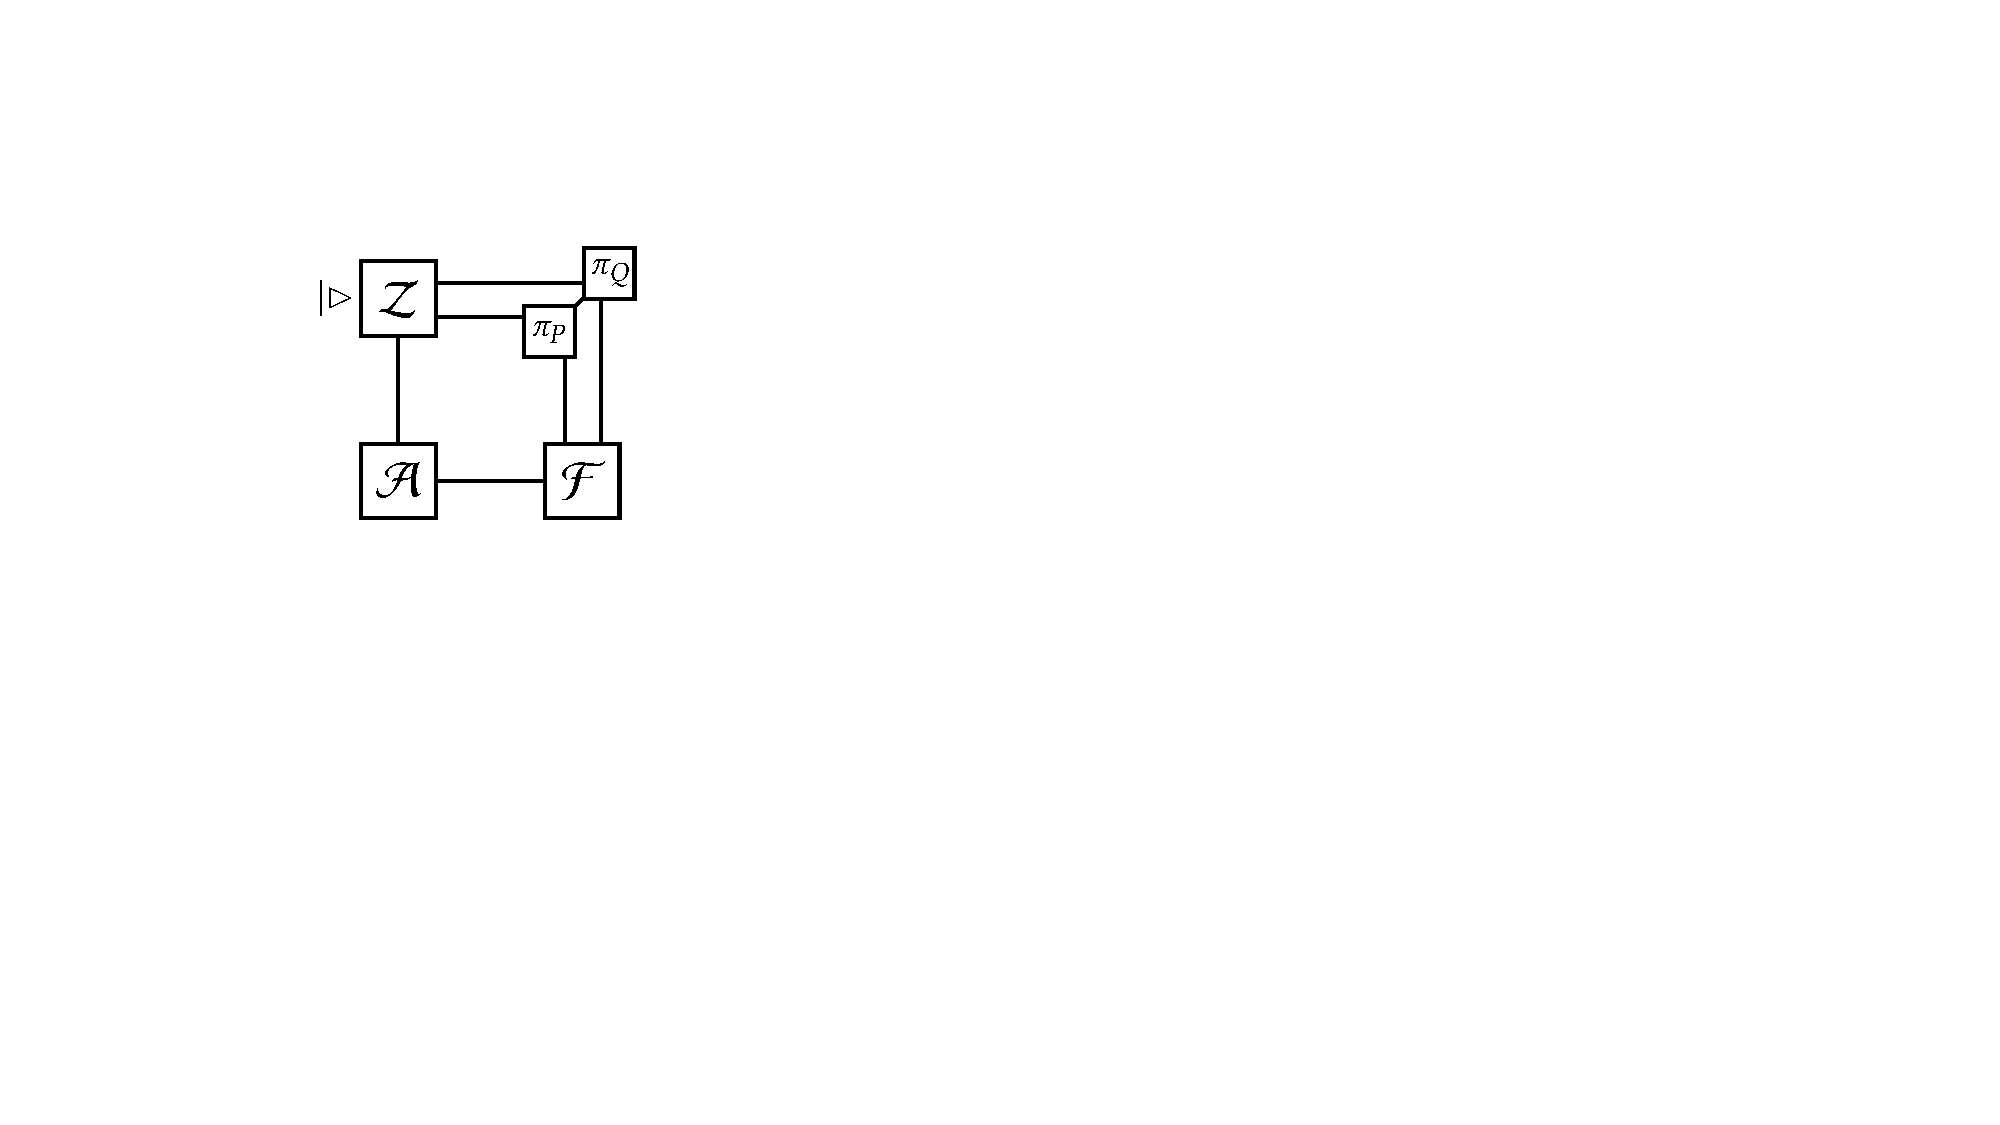
\includegraphics[width=0.4\linewidth]{graphics/execUC}
%  \caption{UC execution.}
%  \label{fig:execUC}
%\end{figure}

\subsection{The UC Framework, Concretely}
\label{subsec:concrete-uc}

\setlength\intextsep{0pt}
\setlength{\columnsep}{10pt}
\begin{wrapfigure}{R}{0.15\textwidth}
\centering
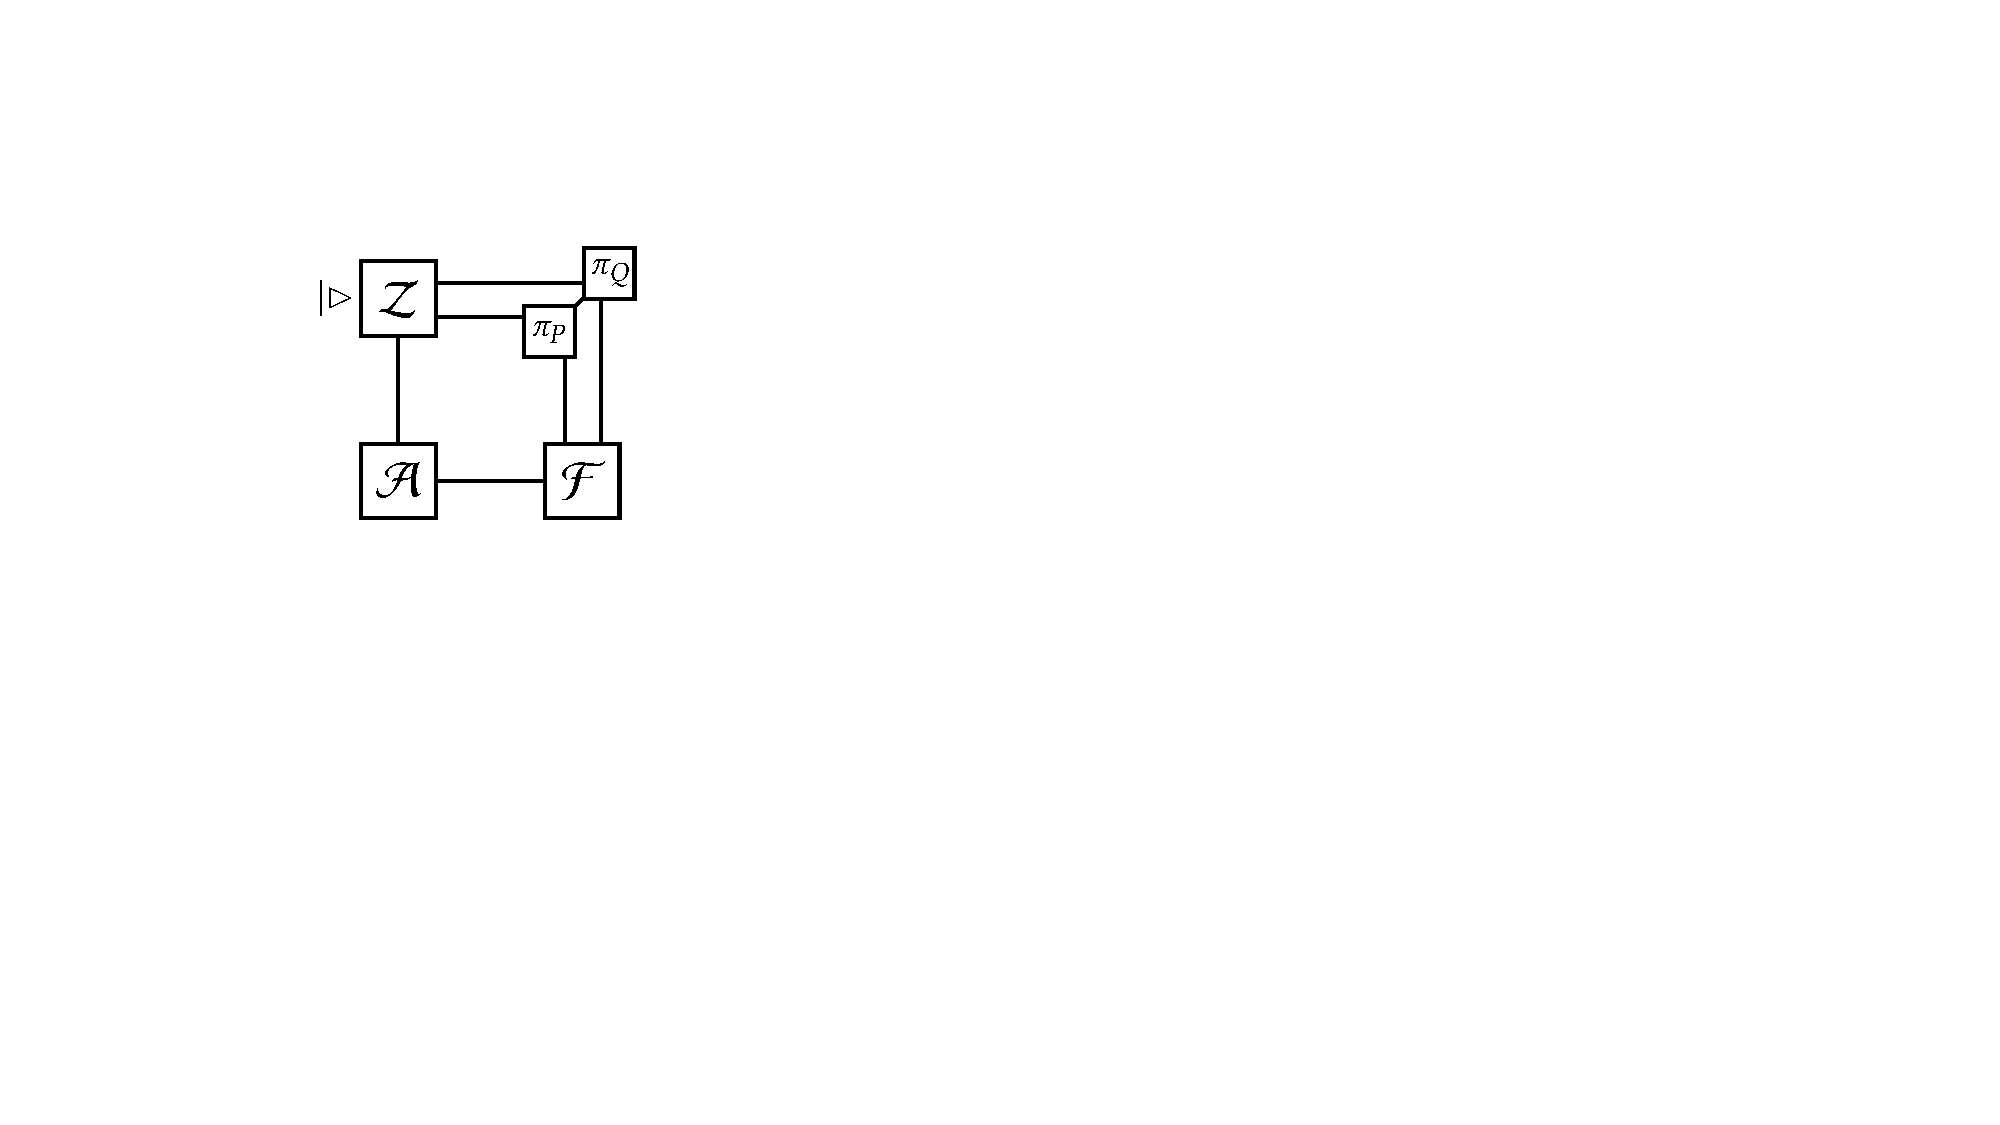
\includegraphics[width=0.15\textwidth]{graphics/execUC}
\caption{\textsf{execUC}.}
\label{fig:execUC-diagram}
\end{wrapfigure}
The first challenge in SaUCy is to define the UC execution model in ILC.  In
principle, this is simple and routes messages as illustrated in
Figure~\ref{fig:execUC-diagram} to the right. For demonstration, we only show
the case of two-party protocols (\`{a} la Simplified
UC~\cite{canetti2015simpler}), which will suffice for our example of
instantiating universally composable commitments.  Also, we will only aim to
show the case of \emph{static} corruptions, in which parties are corrupted at
the onset of the execution. This is in contrast to \emph{adaptive} corruptions,
in which parties can be corrupted as the execution proceeds.

The details require some careful programming, since the adversary gets to send messages on behalf of corrupted parties.
\lstinputlisting[style=myilc]{listings/simp-suc.ilc}
\noindent
The function \textsf{execUC} is parameterized by an environment \textsf{z},
protocol parties \textsf{p} and \textsf{q}, an adversary \textsf{a}, an ideal
functionality \textsf{f}, a security parameter \textsf{k}, a random bitstring
\textsf{r}, and a static corruption model \textsf{crupt :: !Crupt}. The
\textsf{Crupt} datatype is defined below, with its variants denoting the cases
when party \textsf{p} is corrupt, party \textsf{q} is corrupt, or no party is
corrupt, respectively.

\lstinputlisting[style=myilc]{listings/crupt.ilc}

\noindent It first allocates the required channels (see
Figure~\ref{fig:execUC-diagram}), and then splits a random bitstring,
distributing pieces to each of the parties as they are run.  Note that each
protocol party is run in a wrapper function, which determines its behavior based
on whether or not it is corrupted. If a party is corrupted, then the adversary
masquerades as the party.

Note that for space and readability, we elide channel allocation
and distribution (with ellipses) and abbreviate the type signature (e.g.,
$X_{\mathsf{z}}$ is the type of \textsf{z}), but more details can be found
in Appendix~\ref{sec:full-execUC}.

%$\{(\mathsf{m}_{\mathsf{f}},\mathsf{m}_{\mathsf{a}},\mathsf{m_{\mathsf{z}}) \mid \mathsf{m}_{\mathsf{f}} || (\mathsf{m}_{\mathsf{a}} || (\mathsf{R} || (\mathsf{R} || \mathsf{m}_{\mathsf{z}}))) => \mathsf{m}_{\mathsf{e}}}\}$

\begin{comment}
\begin{itemize}[leftmargin=*]
  \item \emph{Environment.} The environment's program defines interactions with
    the protocol parties and the adversary, which have different programs in the
    real world and the ideal world (see below). Its job is to distinguish which
    of the worlds it is interacting with.
  \item \emph{Protocol.} In the real world, the program of the protocol parties
    correspond to actual programs for running the protocol. In the ideal world,
    the protocol parties are simply dummy parties, which relay messages between
    the environment and the functionality.
  \item \emph{Adversary.} In the real world, the adversary is simply the dummy
    adversary, which relays messages between the environment and either the
    functionality or a corrupted party. In the ideal world, the adversary is a
    simulator, which must mimic the attack of any real world adversary, but in
    the ideal world.
  \item \emph{Functionality.} In the real world, the functionality is any
    functionality that the real world protocol makes calls to (if any). In the
    ideal world, the functionality is the specification for the protocol under
    analysis.
  \item \emph{Security parameter.} Each process is handed a security parameter
    (a natural number), and must run in a number of steps polynomial in this
    security parameter. We have more to say on this later.
  \item \emph{Corruptions.} The possible corruption models are either party
    \textsf{p} is corrupt, party \textsf{q} is corrupt, or no parties are
    corrupt, which are defined in the following datatype:
    \lstinputlisting[style=myilc]{listings/crupt.ilc}
\end{itemize}
\end{comment}

%For a real world execution, the protocol parties contain code for running the
%actual protocol under analysis, the adversary is the dummy adversary, and the
%ideal functionality is any functionality that the protocol makes calls to (if
%any). For an ideal world execution, the protocol parties are simply dummy
%parties, the adversary is a simulator, and the ideal functionality is a
%specification for the protocol under analysis. The environment has the ability
%to interact with each of the executions as they evolve. For the simulation to be
%good, the environment should not be able to distinguish which of the executions
%it is interacting with.

\subsection{Probabilistic Polynomial Time in ILC}
\label{subsec:ppt}
The goal of cryptography reduction is to relate every bad event in the protocol to a \emph{probabilistic polynomial time computation} that solves a hard problem.
The ILC typing rules do not guarantee termination, let alone polynomial time normalization, so we must tackle this in metatheory.
Also, since ILC is effectively deterministic (confluent), we will need to express random choices some other way.
To meet these needs we define a judgment about ILC terms that take a security parameter and a  stream of random bits.

\begin{definition}[Polynomial time normalization]
  \begin{comment}
  Consider a term \textsf{e} with the type
  \[\emptyctxt ;\emptyctxt |- \mathsf{e} : \tyBang{\tyNat} \multimap \tyBang{[\tyBit]}~{\multimap}_m~\tyBang{\tyBit},\]
  where the first argument is a security parameter and the second argument is a
  random bitstring.\footnote{The definition of polynomial time normalization
    applies similarly to a term \textsf{e} of type $\tyBit$ where the security
    parameter and random bitstring are free variables in \textsf{e}.} We say
  that \textsf{e} is polynomial time normalizable, written \textsf{poly(e)}, if
  for all security parameters \textsf{k} and all random bitstrings \textsf{r},
  where the length of \textsf{r} is polynomial in the security parameter
  \textsf{k}, the term \textsf{e k r} normalizes to a value \textsf{v} in a
  polynomial (in \textsf{k}) number of steps.
  \end{comment}
  The judgment that \textsf{e} is polynomial time normalizable, written \textsf{PPT e}, is defined as follows:
  \begin{mathpar}
    \Infer{ppt}
    {\emptyctxt ~; \emptyctxt |- e : \tyBang{\tyNat} \multimap \tyBang{[\tyBit]} {\multimap}_{m}
      \tyBang{\tyBit}\\
    \forall~\mathsf{k} \in \tyNat.~\forall~r \in {[\tyBit]}^{(poly(\mathsf{k}))}.~\mathsf{e~!k~!r}~{->}^{poly(\mathsf{k})}~\mathsf{v}}
    {\keyword{PPT}~ \mathsf{e} }
  \end{mathpar}
  This says that if for all security parameters \textsf{k} and all bitstrings
  \textsf{r} with length polynomial in \textsf{k} the term \textsf{e~!k~!r}
  normalizes to a value \textsf{v} in $poly(\mathsf{k})$ steps.
  Note that the normalization is polynomial time for all $\mathsf{r}$.
\end{definition}

\begin{definition}[Value Distribution] 
  Because processes are confluent, we know that if $\mathsf{e~!k~!r}~{->}^{*}~\mathsf{v}$
  then the value $\mathsf{v}$ is unique.  We can therefore define the
  probability distribution ensemble $D(\mathsf{e}) = \{ D_{\mathsf{e,k}}
  \}_\mathsf{k}$ of values given a uniform distribution $U_k$ over
  $\mathsf{k}$-bit strings $\mathsf{r}$, where
\[
D_{\mathsf{e},\mathsf{k}}(\mathsf{v}) = \sum_{\mathsf{r} \in R} U_{\mathsf{k}}(\mathsf{r}), \quad \textnormal{for~} R = \{ \mathsf{r} ~|~ \mathsf{e~!k~!r}~{->}^{*}~\mathsf{v} \}.
\]
\end{definition}

\begin{definition}[Indistinguishable]
 Finally, we will often need a notion of indistinguishability, roughly corresponding to statistical indistinguishability of value distributions ${D(\mathsf{e}_1) \sim D(\mathsf{e}_2)}$. However, we need to be clear on when polynomial time normalization is an assumption or a proof obligation.
  To simplify things later, we define a partial order $\mathsf{e}_1 \le \mathsf{e}_2$, which captures that $e_2$ must be PPT if $e_1$ is PPT, and if so, that their value distributions are similar.
  \begin{mathpar}
    \Infer{indist}
    {\keyword{PPT}~ \mathsf{e}_1 \implies (\keyword{PPT}~ \mathsf{e}_2 ~~\keyword{and}~~
    {D(\mathsf{e}_1) \sim D(\mathsf{e}_2)})}
    {   \qquad \mathsf{e}_1 \le \mathsf{e}_2 }
  \end{mathpar}
\end{definition}

\subsection{Defining UC Security in ILC}
\label{subsec:uc}
What remains is for us to give a precise definition of secure protocol emulation.
We roughly want to say a protocol $\pi$ emulates $\phi$ if the environment cannot distinguish between the two.
In SaUCy notation we make the functionality explicit, so emulation is actually defined as a relationship between protocol-functionality pairs. Furthermore we make the simulator $\mc{S}$ explicit, so overall we will define a judgment of the form
\[
(\pi, \mc{F}_1) \overset{\mc{S}}\approx (\phi, \mc{F}_2)
\]
%\[
%S ~\keyword{proves}~ (\pi, \mc{F}_1) ~\keyword{emulates}~ (\phi, \mc{F}_2).
%  \]
%  Since the simulator tranlates attacks $\mc{A}$ to the real world, we treat $\mc{S}$ as a function, so $\mc{S A}$ is the ideal world adversary simulating $\mc{A}$.
Since emulation  means that any attack on $\pi$ is also on $\phi$.
We have to translate attacker behaviors of an arbitrary real world adversary $\mc{A}$ to a simulated adversary $\mc{(S~A)}$ in the ideal world.
A first attempt to define this would be
\begin{mathpar}
  \Infer{\st{emulate}}
        {\forall~\mc{A}~\mc{Z}.~ 
         \mathsf{execUC}\ \mc{Z}\ \pi\ \mc{F}_1\ \mc{A} \le
         \mathsf{execUC}\ \mc{Z}\ \phi\ \mc{F}_2\ (\mc{S}~\mc{A})}
    {(\pi, \mc{F}_1) \overset{\mc{S}}\approx (\phi, \mc{F}_2)}
  \end{mathpar}

\noindent However this definition is vacuous: a degenerate protocol $\pi$ can emulate anything simply failing to be $\keyword{PPT}$, e.g. by diverging. To put it another way, the problem is the definition imposes a proof obligation on the simulator $\mc{S}$ but not on $\pi$. What we want to say is that the \emph{real world} protocol $(\pi, \mc{F}_1)$ must be well behaved whenever the \emph{ideal world} $(\phi, \mc{F}_2)$ is.
However, even a reasonable protocol can result in non-PPT executions if paired with a divergent environment. We therefore need to express a judgment $\keyword{Good}$ to describe environments that are well behaved in the ideal world:
\begin{mathpar}
  \Infer{good}
        {\keyword{PPT}~(\mathsf{execUC}~\mc{Z}~\phi~1_\mc{A}~\mc{F}_2)}
        {\keyword{Good}~\phi~\mc{F}_2~\mc{Z}}
\end{mathpar}
\noindent Notice that this constraint has the dummy adversary $1_\mc{A}$.
%, even though it is written for the ideal world, unlike in the dummy lemma.
This is without loss of generality in the sense that $\keyword{Good}~\phi~\mc{F}_2~Z$ implies that for any $\mc{A}$, we could have a $\mc{Z'}$ such that
\[
\mathsf{execUC}~\mc{Z} ~\phi  ~\mc{A}~\mc{F}_2 \le
\mathsf{execUC}~\mc{Z'}~\phi~1_\mc{A}~\mc{F}_2
\]
\noindent We can now repair the emulation definition using this constraint.
\begin{definition}[Protocol Emulation]
  The judgment that one protocol-functionality pair $(\pi, \mc{F}_1)$  securely emulates another $(\phi, \mc{F}_2)$ (as proven the simulator $\mc{S}$) is defined as follows:
  \begin{mathpar}
  \Infer{{emulate}}
        {\forall~\mc{A}~\mc{Z}.~ \keyword{Good}~\phi~\mc{F}_2~\mc{Z} =>\\\\
         \mathsf{execUC}\ \mc{Z}\ \pi\ \mc{F}_1\ \mc{A} \le
         \mathsf{execUC}\ \mc{Z}\ \phi\ \mc{F}_2\ (\mc{S}~\mc{A})}
        {(\pi, \mc{F}_1) \overset{\mc{S}}\approx (\phi, \mc{F}_2)}
  \end{mathpar}
\end{definition}

\subsection{A composition theorem in SaUCy}
\label{subsec:composition}

\begin{figure}
  \centering
  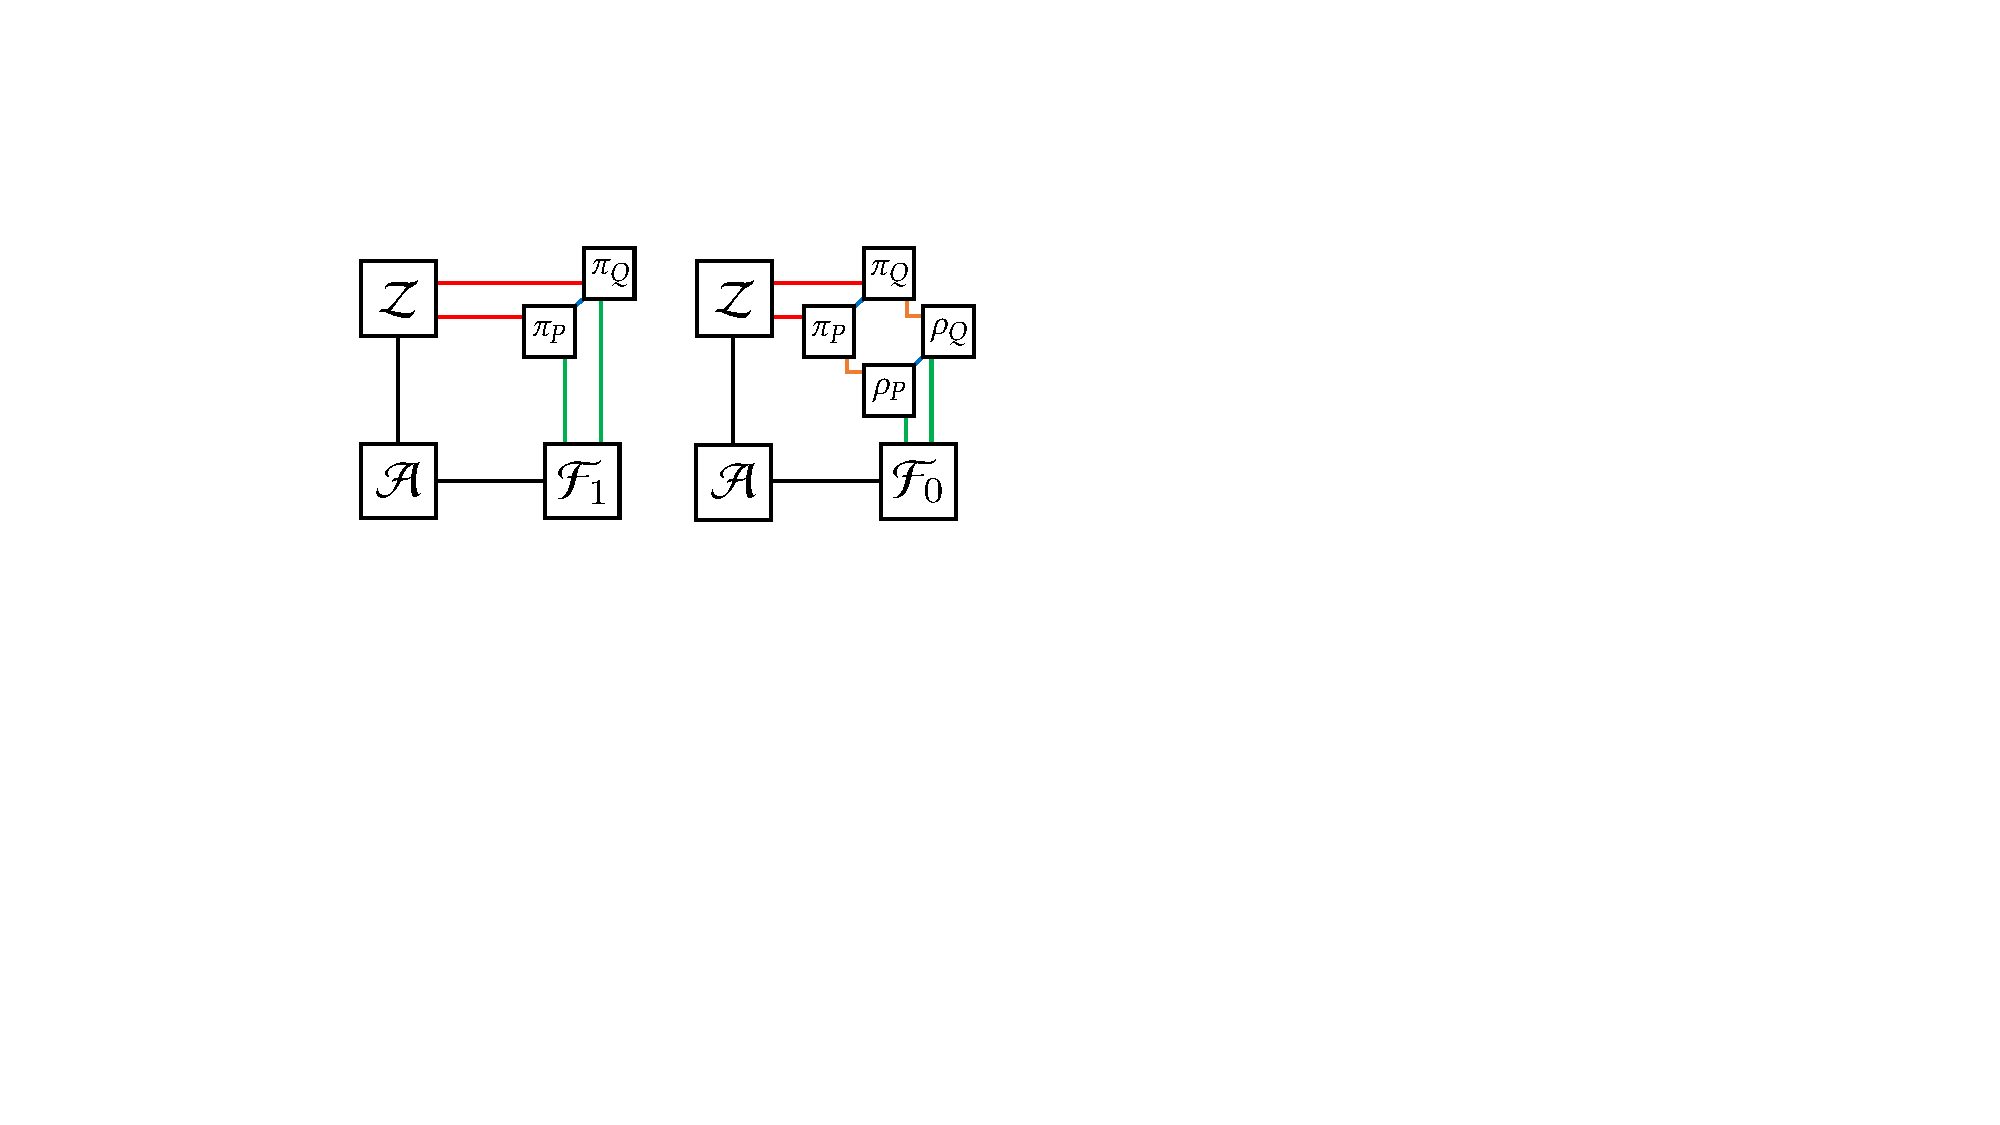
\includegraphics[width=0.85\linewidth]{graphics/protocol-composition}
  \caption{Protocol composition diagram.}
  \label{fig:protocol-composition}
\end{figure}

As a first usage of SaUCy, work through the development of a composition
operator, and give a composition theorem explaining its use.

\todo{Explain more the importance of composition operators}

Essentially, our operator is the notion of UC-realizes. We can now state useful
composition operators, simplifying lemmas, and notation. For brevity, we pack
several notions from UC into a single alternate definition: UC-realizes.

\begin{definition}[UC-realizes]
  Protocol $\pi$ with $\mc{F}_0$ realizes $\mc{F}_1$, written
  $\mc{F}_0 \yrightarrow{$\pi$} \mc{F}_1$, if for all environments $\mc{Z}$,
%  if $\keyword(\mc{Z}, \pi, \mc{F}_0, \mc{A}_{\mathbbm{1}})$, then
%  $|- \keyword{polyUC}(\mc{Z}, \pi_{\mathbbm{1}}, \mc{F}_1, \mc{S})$, and the
  %  following statistical indistinguishability relation holds

  \begin{mathpar}
    \Infer{realizes}
          {\forall~\mc{Z}.~ \keyword{Good}~\phi~\mc{F}_2~\mc{Z} =>\\\\
            \mathsf{execUC}\ \mc{Z}\ \pi\  \mc{F}_1\ 1_\mc{A} \le
            \mathsf{execUC}\ \mc{Z}\ \phi\ \mc{F}_2\ \mc{S}}
          {\mc{F}_0 \yrightarrow{$\pi$} \mc{F}_1}
  \end{mathpar}
\end{definition}

The idea is that the environment can arbitrarily and adaptively choose
inputs to the protocol $\phi$. So when we compose with an arbitrary other
protocol $\rho$, it is not any worse than what the environment could have
done. It essentially creates a proof obligation to ensure isolation of the
protocols.  While the intended use of universal composition is to replace an
ideal functionality with a protocol that securely realizes it, we define
protocol composition \todo{Let's just call it protocol composition, not
  universal composition. It's not really universal.} more generally in terms of
replacing one subroutine protocol with another. Given a protocol $\phi$, a protocol
$\rho$ that makes calls to $\phi$, \todo{instead of ``makes calls'', specify that the
  \textsf{toF} channel of $\rho$ is connected to the \textsf{fromZ} channel of
  $\phi$. } and a protocol $\pi$ that emulates $\phi$, then $\rho^{\phi -> \pi}$ is identical to
$\rho$ with the following modifications:
\begin{itemize}[leftmargin=*]
  \item When $\rho$ writes to $\phi$, $\rho^{\phi -> \pi}$ writes to $\pi$.
  \item When $\rho^{\phi -> \pi}$ receives a message from $\pi$, proceed as $\rho$ would when
    it receives the same message from $\phi$.
\end{itemize}

\begin{figure}
\lstinputlisting[style=myilc]{listings/compose.ilc}
\caption{Protocol composition operator.}
\label{fig:composition-operator}
\end{figure}

From UC-realizes, we can conclude the original UC formulation for arbitrary
composition:
\begin{theorem}[Composition Theorem]
  If $\mc{F}_0 \yrightarrow{$\pi$} \mc{F}_1$, then for all $\rho$ we
  have that $(\rho^{\pi}, \mc{F}_0)$ emulates $(\rho, \mc{F}_1)$.
\end{theorem}

\subsection{Instantiating UC Commitments}
\label{subsec:example}
We walk through the development of a UC instantiation for commitments.  UC
commitments can be instantiated with standard cryptographic assumptions, for
example the RSA problem.  Also rely on a ``trusted setup'', or common reference
string, essentially public parameters generated ahead of time (modeled as an
ideal functionality FCRS).

Instantiation proofs in UC follow a standard rhythm. We start with a security
definition as an ideal functionality, give the protocol, construct a simulator,
and finally complete the relational analysis on paper.  UC commitments are
reasoned to be secure assuming a common reference string is suitably generated.
To model the cryptography we extend ILC with additional syntax.

The functionality FCom has already been defined.
\todo{Recap the proof obligation}

\paragraph{Extending ILC with cryptographic primitives.}
\todo{Still lots of changes to make here.} UC Commitments are realized from
cryptographic primitives, such as pseudorandom trapdoor permutations. This
requires us to extend the syntax. The semantics are written in terms of the
cryptographic objects themselves, and we still arrive at a computational
reduction for our security proof.

The new syntactic forms are \textsf{kgen}, \textsf{tdp}, \textsf{inv}, and
\textsf{hc} with the static and dynamic semantics shown in
Figure~\ref{fig:extended-ilc}. The key generation function \textsf{keygen}
generates, on input $1^n$ (security parameter), a random public key $v_{pk}$ and
a trapdoor $v_{td}$. The trapdoor permutation function \textsf{tdp} computes, on
input key $v_k$ and bitstring $v_{in}$, a bitstring $v_{out}$. The hardcore
predicate function \textsf{hc} generates, on input trapdoor permutation
$f_{v_k}$.

\begin{figure*}
  \begin{grammar}
    Expressions
    & $e$
        &$\bnfas$&
        $\eKGen{e} \bnfalt \eTdp{e_1}{e_2} \bnfalt \eHc{e}$
  \end{grammar}
  
  \judgbox{\Delta ; \Gamma |- e : A |> m}{~~Under $\Delta$ and $\Gamma$, expression~$e$ has
  intuitionistic type $A$ and mode $m$.}
  \begin{mathpar}
  \Infer{kgen}
  {\Delta ; \Gamma |- e : [\tyBit]}
  {\Delta; \Gamma |- \eKGen{e}: [\tyBit]}
  %
  \and
  %
  \Infer{eTdp}
  {\Delta_1; \Gamma |- e_1 : [\tyBit]\\
   \Delta_2; \Gamma |- e_2 : [\tyBit]}
  {\Delta_1, \Delta_2; \Gamma |- \eTdp{e_1}{e_2}: [\tyBit]}
  %
  \and
  %
  \Infer{hc}
  {\Delta; \Gamma |- e : \tyArr{[\tyBit]}{}{\tyArr{[\tyBit]}{}{[\tyBit]}}}
  {\Delta; \Gamma |- \eHc{e}: \tyBit}
  \end{mathpar}
  
  \judgbox{\Store_1 ; e_1 ---> \Store_2 ; e_2}{~~Under store $\Store_1$,
    expression~$e_1$ reduces to~$\Store_2 ; e_2$.}
  \begin{mathpar}
  \Infer{kgen}
  {\keyword{\textbf{Gen}}(n) = (v_{pk}, v_{td}) \\ v_{pk}, v_{td} \in \{0,1\}^n}
  { \Store ; \eKGen{n} ---> \Store ; (v_{pk}, v_{td})}
  \and
  \Infer{tdp}
  {\mathbf{f}_{v_k}(v_i) = v_o \\ \mathbf{f} \colon \{0,1\}^n -> \{0,1\}^n -> \{0,1\}^n}
  { \Store ; \eTdp{v_k}{v_i} ---> \Store ; v_o }
  \and
  \Infer{hc}
  {\keyword{\textbf{Hc}}(\mathbf{f}_{v_k}) = v \\ \keyword{\textbf{Hc}} \colon
  (\{0,1\}^n -> \{0,1\}^n) -> \{0, 1\}}
  { \Store ; \eHc{f_{v_k}} ---> \Store ; v}
  \end{mathpar}
%  \begin{mathpar}
%    G_{pk}(r) = (f^{(3n)}_{pk}(r), B(f^{(3n-1)}_{pk}(r)), \ldots, B(f_{pk}(r)), B(r))
%  \end{mathpar}
  \caption{ILC extended with trapdoor permutations.}
  \label{fig:extended-ilc}
\end{figure*}


\[ G_{pk}(r) = \big(f_{pk}^{(3n)}(r), B(f_{pk}^{(3n-1)}(r)), \ldots, B(f_{pk}(r)), B(r)\big)\]

\lstinputlisting[style=myilc]{listings/prg.ilc}

\begin{algorithm}
\SetAlgorithmName{Protocol}{protocol}{List of Protocols}
\DontPrintSemicolon

\SetKwBlock{Parameters}{\textnormal{\textsf{Public strings}:}}{}
\Parameters{
  $\sigma$: Random string in $\{0,1\}^{4n}$\;
  ${pk}_0, {pk}_1$: Keys for generator $G_{k} \colon \{0,1\}^n \to \{0,1\}^{4n}$
}\smallskip
\SetKwBlock{Commit}{\textnormal{\textsf{Commit}($b$):}}{}
\Commit{
  $r \leftarrow \{0, 1\}^n$\;
  $x \coloneqq G_{{pk}_b}(r)$\;
  if $b=1$ then $x \coloneqq x \oplus \sigma$\;
  Send $(\mathsf{Commit}, x)$ to receiver.\;
  Upon receiving $(\mathsf{Commit}, x)$ from $A$, $B$ outputs $(\mathsf{Receipt})$.
}\smallskip

\SetKwBlock{Decommit}{\textnormal{\textsf{Decommit}($x$):}}{}
\Decommit{
  Send $(b, r)$ to receiver.\;
  Receiver checks $x = G_{{pk}_b}(r)$ for $b = 0$, or $x = G_{{pk}_b}(r) \oplus \sigma$
  for $b = 1$. If verification succeeds, then $B$ outputs $(\mathsf{Open}, b)$.
}
\caption{Universally Composable Commitment}
\label{alg:com}
\end{algorithm}

\begin{figure}
\lstinputlisting[style=myilc]{listings/ucc.ilc}
\caption{Universally composable commitment in ILC.}
\label{fig:ucc}
\end{figure}

\paragraph{Commitment Protocol.}
We defer the protocol to the appendix.

\paragraph{Defining the simulator.}

\paragraph{Relational argument.}

\subsection{Reentrancy in SaUCy}
\label{subsec:reentrancy}

The cryptography community has recently identified several subtleties in defining UC ideal functionalities that relate to ``reentrancy'' and scheduling of concurrent code;
as a consequence, many functionalities in the literature turn out to be ill-defined~\cite{camenisch2016universal}.
This subtle definitional issue, although important for the well-foundedness of security claims,
is not ``cryptographic'' in nature, and is better addressed from the PL viewpoint.
To illustrate, consider the following fragment of (untyped) ILC syntax, which allows an adversary to control the delivery schedule of messages from $P$ to $Q$ (an asynchronous channel):
\lstinputlisting[style=myilc]{listings/reentrant.ilc}
After receiving input from party $P$, it
notifies the adversary, then forks a background thread to wait for \textsf{OK} before
delivering the message.
This introduces a race condition: suppose input message $m_1$ is sent by $P$, but then the adversary $\mathcal A$, before sending \textsf{OK}, instead returns control to $\mathcal Z$, which passes $P$ a second input $m_2$. Now there are two queued messages; which one gets delivered first when the adversary sends \textsf{OK}?

To resolve this paradox, notice that fragment is untypeable in ILC.
The race condition occurs because of duplication of the read channel \textsf{frA}.
Since \textsf{frA} is linear in the function body, the function would not be typeable as intuitionistic as required by the \textsf{loop} construct.
Camenisch et al.~\cite{camenisch2016universal} identified several strategies for resolving this problem in UC, which in turn are expressible ILC. One approach is to make the process explicitly sequential, such that the arrival of a second message before the first is delivered causes execution to get stuck:
\lstinputlisting[style=myilc]{listings/reentrant-seq.ilc}
An alternative is to discard such messages arriving out of order, returning them to sender; this can be expressed in ILC using the external choice operator:
operator,
\lstinputlisting[style=myilc]{listings/reentrant-ignore.ilc}


\section{UC Theory}
\label{sec:uc}

\begin{theorem}[Protocol Emulation]

\end{theorem}


\section{Related Work}
\label{sec:related}

\begin{enumerate}[leftmargin=*]
  \item Symbolic UC~\cite{bohl2016symbolic} transports ideas from the UC
    framework to the symbolic model of cryptography, in which cryptographic
    operations are abstracted as a term process algebra (specifically, a variant
    of the applied $\pi$-calculus) and adversary capabilities are defined by
    deduction rules over these terms. In particular, they show that certain
    aspects of the UC framework, such as ideal functionality specifications and
    UC composition, still carry over to the symbolic model. They are also able
    to show that certain results, such as the impossibility of UC commitments in
    the standard model of cryptography, can still be observed in the symbolic
    model. Although this abstract vantage point leads to simpler security proofs
    that can be amenable to automated reasoning, security guarantees derived
    from symbolic analyses are not as strong as those from computational
    analyses considered in UC and in cryptography more broadly.
  \item RSIM~\cite{backes2007reactive}
  \item CertiCrypt~\cite{barthe2009formal} is a framework (built on
    Coq~\cite{barras1997coq}) that supports machine-checked game-based proofs of
    security. It includes tools to reason about the equivalence of probabilistic
    programs, a relational Hoare logic, a theory of observational equivalence,
    verified program transformations, and game-based techniques.  Their
    experience shows that the type system and automated tactics provide valuable
    information in debugging proofs.
  \item EasyCrypt~\cite{barthe2011computer} is follow-up work on CertiCrypt,
    which permits more automation and shorter proof scripts. \todo{Details on
      their imperative language?}
  \item ProVerif~\cite{blanchet2010proverif} is a tool for symbolically
    analyzing cryptographic protocols. It relies on the Horn theory approach, in
    which protocols and intruders are modeled as Horn theories. Protocols are
    analyzed with respect to an unbounded number of protocol sessions that may
    run concurrently and there is no bound on the number of messages an
    adversary can generate. Verifying security properties, such as secrecy,
    boils down to solving the derivation problem for Horn theories. Protocols
    can be specified as either Horn theories, or in a variant of the applied
    process calculus, which is translated into Horn theories.
  \item CryptoVerif~\cite{blanchet2007cryptoverif} works directly in the
    computational model. Produces game-based proofs valid for any number of
    sessions of the protocol in the presence of an active adversary. Games are
    represented in a process calculus inspired by the $\pi$-calculus,
    \cite{laud2005secrecy}, and \cite{mitchell2006probabilistic}. The calculus
    has a probabilistic semantics.
  \item Cryptol~\cite{lewis2003cryptol} allows for writing executable
    specifications of a protocol, which are amenable to testing, theorem
    proving, verifying equivalence to their own programs, and even generating
    code or hardware from the specification.
  \item $\text{F}^{\star}$~\cite{swamy2016dependent} is a language that functions as
    a proof assistant (SMT automation and constructive proofs using dependent
    types) as well as a general-purpose, verification-oriented programming
    language.
  \item Spi calculus~\cite{abadi1999calculus} is an extension of the
    $\pi$-calculus with cryptographic primitives. In the spi calculus, as in the
    $\pi$-calculus, channels can be passed over channels, and its scoping rules
    guarantee that an attacker cannot access a channel it is not explicitly
    given (scoping is the basis of security). \todo{Why do we prevent passing channels
    over channels in SaUCy?} The spi calculus allows expressing security
    guarantees as equivalences between spi calculus processes. For example, we
    can say that a protocol maintains the secrecy of a value $x$ by stating that
    the protocol with $x$ is equivalent to the protocol with $x'$, for every
    $x'$. Here, equivalence means equivalence in the eyes of an arbitrary
    environment that interacts with the protocol. \todo{They cannot take the
      standard bisimilarity relation as our notion of equivalence. Why?}

    Although equivalence makes reference to the environment, we do not need to
    give a model of the environment explicitly. Instead, the environment can be
    an arbitrary pi calculus process. In sum, their approach uses the powerful
    scoping constructs of the $\pi$-calculus, the definition of an environment as
    an arbitrary spi calculus process, and the representation of security
    properties (both integrity and security) as equivalences. However, the spi
    calculus does not include any notion of probability or complexity, so it can
    be a useful foundation for symbolic cryptography, but not computational
    cryptography.

    In $\pi$-calculus, the scope of a channel can change during a
    computation. When a process sends a restricted channel to a process outside
    the scope of the restriction, the scope is said to extrude. Why do we
    disallow extrusion in SaUCy? A central idea in spi calculus is to use
    restriction and extrusion to keep track of secret values.

    Another difference is that channels are bidirectional. 
  \item Applied $\pi$-calculus~\cite{abadi2001mobile} is a similar extension to
    the $\pi$-calculus. Here, there is no need to craft a special calculus and
    develop its proof techniques for each choice of cryptographic
    operation. Includes name restriction and variable restriction (as in the spi
    calculus), so fresh channels, nonces, and keys can be represented as new
    names. Attacks against protocols rely on equational properties.

    Example for one-way hash functions: Represent hash functions with a unary
    function symbol \textsf{h} (without any equational properties). The absence
    of an inverse for \textsf{h} models one-wayness. In comparison with spi
    calculus, the applied pi calculus permits a more uniform and versatile
    treatment of cryptographic functions (e.g., one-way hash functions,
    encryption/decryption, signatures, XOR), their variants, and their
    properties. \todo{Not clear to me why this is the case.} The spi calculus
    developed the idea that the context represents an active attacker, and
    equivalences capture authenticity and secrecy properties (same as here).
  \item Wysteria?~\cite{rastogi2014wysteria}
  \item Lambda auth?~\cite{miller2014authenticated}
  \item Fowler \etal~\cite{fowler2018session} develop a session typed
    programming language that is confluent. Only allows for fixed and two-party
    communications.
  \item Sequentiality and the $\pi$-calculus~\cite{berger2001sequentiality}. The
    authors developed a typed $\pi$-calculus that uses affineness and stateless
    replication to achieve deterministic computation. \todo{More details.}
  \item Secrecy types for a simulatable cryptographic
    library~\cite{laud2005secrecy}. They define a language for cryptographic
    protocols similar to the spi calculus and give it a semantics using the
    computational model of cryptography. They propose a type system for their
    language and show that if a protocol types, then it preserves the secrecy of
    messages given to it by users. The semantics of their calculus is
    deterministic. When complexity-theoretic security definitions are used,
    nondeterminism cannot be employed. The adversary is allowed to choose which
    thread handles the received message. 
  \item PPT process calculus for analysis of cryptographic
    protocols~\cite{mitchell2006probabilistic, lincoln1998probabilistic}. To
    avoid inconsistency between security and nondeterminism, messages are
    schedule probabilistically instead of nondeterministically. They prove that
    any process expression halts in polynomial time, and they define a form of
    asymptotic protocol equivalence that allows security properties to be
    expressed using observational equivalence, a standard relation that involves
    quantifying over all environments that might interact with the protocol. A
    limitation of deterministic or nondeterministic settings is the inability to
    analyze probabilistic protocols. Traditional nondeterministic scheduling
    means that an adversary has exponential computing power. With
    nondeterministic scheduling, an adversary can guess a $k$-bit key by
    concatenating $k$ bits. The combination of nondeterminism and bit-level
    representation of encryption keys renders any encryption function insecure.
\end{enumerate}


\section{Future Work}
\label{sec:future}


\section{Conclusion}
\label{sec:conclusion}


\bibliography{bibs/references}

\appendix

\onecolumn
\section{Algorithmic Typing Rules}
\label{sec:algo-type-check}
\ \\

\begin{figure*}[h]
\centering
\judgbox{\Delta_{in} ; \Gamma_1 |- e : \Delta_{out}; \Gamma_2; A}{~~Under $\Delta_{in}$ and
  $\Gamma_1$, expression~$e$ results $\Delta_{out}$ and $\Gamma_2$ and has intuitionistic type $A$.}
\begin{mathpar}
\Infer{a-var}
{\Gamma(x) = A}
{\Delta; \Gamma |- x : \Delta; \Gamma; A}
%
\and
%
\Infer{a-unit}
{ }
{\Delta ; \Gamma |- \eUnit : \Delta; \Gamma; \tyUnit}
%
\and
%
\Infer{a-pair}
{\Delta_1; \Gamma |- e_1 : \Delta_2; \Gamma; A_1\\\\
\Delta_2; \Gamma |- e_2 : \Delta_3; \Gamma; A_2}
{\Delta_1; \Gamma |- \ePair{e_1}{e_2} : \Delta_3; \Gamma;  \tyProd{A_1}{A_2}}
%
\and
%
\Infer{a-inj}
{i \in \{1, 2\}\\\\
\Delta_1; \Gamma |- e : \Delta_2; \Gamma; A_i}
{\Delta_1 ; \Gamma |- \eInj{i}{e} : \Delta_2; \Gamma; \tySum{A_1}{A_2}}
%
\and
%
\Infer{a-ref}
{\Delta_1; \Gamma |- e : \Delta_2; \Gamma; A}
{\Delta_1; \Gamma |- \eRef{e} : \Delta_2; \Gamma; \tyRef{A}}
%
\and
%
\Infer{a-split}
{\Delta_1; \Gamma |- e_1 : \Delta_2; \Gamma; \tyProd{A_1}{A_2}\\\\
\Delta_2; \Gamma,x_1:A_1, x_2: A_2 |- e : \Delta_3; \Gamma; B}
{\Delta_1; \Gamma |- \eSplit{e_1}{x_1}{x_2}{e_2} : \Delta_3; \Gamma; B}
%
\and
%  
\Infer{a-case}
{\Delta_1; \Gamma |- e : \Delta_2; \Gamma; \tySum{A_1}{A_2}\\\\
\Delta_2; \Gamma,x_1:A_1 |- e_1 : \Delta_3; \Gamma; B\\\\
\Delta_2; \Gamma,x_2:A_2 |- e_2 : \Delta_3; \Gamma; B}
{\Delta_1; \Gamma |- \eCase{e}{x_1}{e_1}{x_2}{e_2} : \Delta_3; \Gamma; B}
%
\and
%
\Infer{a-get}
{\Delta_1; \Gamma |- e : \Delta_2; \Gamma; \tyRef{A}}
{\Delta_1; \Gamma |- \eGet{e} : \Delta_2; \Gamma; A}
%
\and
%
\Infer{a-set}
{\Delta_1; \Gamma |- e_1 : \Delta_2; \Gamma; \tyRef{A}\\\\
\Delta_2; \Gamma |- e_2 : \Delta_3; \Gamma; A}      
{\Delta_1; \Gamma |- \eSet{e_1}{e_2} : \Delta_3; \Gamma; \tyUnit}
%
\and
%
\Infer{a-fix}
{\emptyctxt; \Gamma,x : \tyArr{A}{\footnotesize m}{A} |- e : \emptyctxt; \Gamma; \tyArr{A}{\footnotesize m}{A}}
{\Delta; \Gamma |- \eFix{x}{e} : \Delta; \Gamma; \tyArr{A}{\footnotesize m}{A}}
%
\and
%
\Infer{a-let}
{\Delta_1; \Gamma |- e_1 : \Delta_2; \Gamma; A\\\\
\Delta_2; \Gamma, x:A |- e_2 : \Delta_3; \Gamma; B}
{\Delta_1; \Gamma |- \eLet{x}{e_1}{e_2} : \Delta_3; \Gamma; B}
%
\and
%
\Infer{a-let!}
{\Delta_1; \Gamma |- e_1 : \Delta_2; \Gamma; A\\\\
\Delta_2; \Gamma, x:A |- e_2 : \Delta_3; \Gamma; B}
{\Delta_1; \Gamma |- \eLetBang{x}{e_1}{e_2} : \Delta_3; \Gamma; B}
%
\and
%
\Infer{a-abs}
{\emptyctxt ; \Gamma, x:A |- e : \emptyctxt; \Gamma; B}
{\Delta ; \Gamma |- \eLam{x}{e} : \Delta; \Gamma; \tyArr{A}{\footnotesize m}{B}}
%
\and
%
\Infer{a-app}
{\Delta_1; \Gamma |- e_2 : \Delta_2; \Gamma; A\\\\
\Delta_2; \Gamma |- e_1 : \Delta_3; \Gamma; \tyArr{A}{\footnotesize m}{B}}
{\Delta_1; \Gamma |- \eApp{e_1}{e_2} : \Delta_3; \Gamma; B}
%
\and
%
\Infer{a-nu}
{\Delta_1, x_1: \tyRd{A} ; \Gamma, x_2 : \tyWr{A} |- e : \Delta_2; \Gamma; B}
{\Delta_1; \Gamma |- \eNu{(x_1, x_2)}{e} : \Delta_2; \Gamma; B}
%
\and
%
\Infer{a-wr}
{\Delta_1; \Gamma |- e_1 : \Delta_2; \Gamma; A\\\\
\Delta_2; \Gamma |- e_2 : \Delta_3; \Gamma; \tyWr{A}}
{\Delta_1; \Gamma|- \eWr{e_1}{e_2} : \Delta_3; \Gamma; \tyUnit}
%
\and
%
\Infer{a-letrd}
{\Delta_1; \Gamma |- e_1 : \Delta_2; \Gamma; \tyRd{A}\\\\
\Delta_2, x_2 : \tyRd{A} ; \Gamma, x_1 : A |- e_2 : \Delta_3; \Gamma; B}
{\Delta_1; \Gamma |- \eLetRd{x_1}{x_2}{e_1}{e_2} : \Delta_3; \Gamma; B}
%
\and
%
\Infer{a-fork}
{\Delta_1; \Gamma |- e_1 : \Delta_2; \Gamma; A\\\\
\Delta_2; \Gamma |- e_2 : \Delta_3; \Gamma; B}
{\Delta_1; \Gamma |- \eFork{e_1}{e_2} : \Delta_3; \Gamma; B}
%
\and
%
\Infer{a-choice}
{\Delta_1; \Gamma |- e_1 : \Delta_2; \Gamma; A\\\\
\Delta_1; \Gamma |- e_2 : \Delta_2; \Gamma; A}
{\Delta_1; \Gamma |- \eChoice{e_1}{e_2} : \Delta_2; \Gamma; A}
\end{mathpar}

\judgbox{\Delta_{in} ; \Gamma_1 |- e : \Delta_{out}; \Gamma_2; A}{~~Under $\Delta_{in}$ and
  $\Gamma_1$, expression~$e$ results $\Delta_{out}$ and $\Gamma_2$ and has affine type $A$.}
\begin{mathpar}
\Infer{a-avar}
{\Delta(x) = X}
{\Delta; \Gamma |- x : \Delta ; \Gamma; X}
%
\and
%
\Infer{a-bang}
{\emptyctxt ; \Gamma |- e : \emptyctxt ; \Gamma ; A}
{\Delta ; \Gamma |- \eBang{e} : \Delta ; \Gamma ; \tyBang{A}}
%
\and
%
\Infer{a-tensor}
{\Delta_1; \Gamma |- e_1 : \Delta_2 ; \Gamma ; X_1\\\\
\Delta_2; \Gamma |- e_2 : \Delta_3 ; \Gamma ; X_2}
{\Delta_1, \Delta_2; \Gamma |- \eLPair{e_1}{e_2} : \Delta_3 ; \Gamma ; \tyTensor{X_1}{X_2}}
%
\and
%  
\Infer{a-asplit}
{\Delta_1; \Gamma |- e_1 : \Delta_2; \Gamma; \tyTensor{X_1}{X_2}\\\\
\Delta_2,x_1:X_1, x_2: X_2; \Gamma |- e : \Delta_3; \Gamma; Y}
{\Delta_1; \Gamma |- \eLsplit{e_1}{x_1}{x_2}{e_2} : \Delta_3; \Gamma; Y}
%
\and
%
\Infer{a-afix}
{\Delta_1, x : \tyLolli{X}{\footnotesize m}{X}; \Gamma |- e : \Delta_ 2 ; \Gamma ; \tyLolli{X}{\footnotesize m}{X}}
{\Delta_1; \Gamma |- \eLfix{x}{e} : \Delta_2 ; \Gamma ; \tyLolli{X}{\footnotesize m}{X}}
%
\and
\Infer{a-lolli}
{\Delta_1,x:X ; \Gamma |- e : \Delta_2 ; \Gamma ; Y}
{\Delta_1 ; \Gamma |- \eLAM{x}{e} : \Delta_2 ; \Gamma ; \tyLolli{X}{\footnotesize m}{Y}}
%
\and
%
\Infer{a-aapp}
{\Delta_1; \Gamma |- e_2 : \Delta_2; \Gamma; X\\\\
\Delta_2; \Gamma |- e_1 : \Delta_3; \Gamma; \tyLolli{X}{\footnotesize m}{Y}}
{\Delta_1; \Gamma |- \eLapp{e_1}{e_2} : \Delta_3; \Gamma; Y}
\end{mathpar}
\caption{Algorithmic typing rules.}
\label{fig:alg-type-check}
\end{figure*}

\twocolumn
\section{\textsf{execUC}}
\label{sec:full-execUC}

\begin{figure*}
\lstinputlisting[style=myilc]{listings/suc.ilc}
\caption{Full definition of \textsf{execUC}. The channels follow a uniform
naming scheme. The read end of a channel is prefixed with \textsf{r-} and the
write end of a channel is prefixed with \textsf{w-}. The channel \textsf{rZ2P}
denotes the read end of communications from the environment \textsf{z} to the
party \textsf{p}. First, the random bitstring is split amongst each of the five
parties. Then, the functionality, the adversary, and both protocol parties are
spawned in a child process (given the appropriate channels and parameters), and
the process continues as the environment process. Notice that parties are run in
wrapper functions, which alter their behavior depending on whether or not they
are corrupted. If a party is corrupted, then the adversary masquerades as the
party. The mode carried over the rightmost lollipop is $m \in \{(\mathsf{m}_{\mathsf{f}},\mathsf{m}_{\mathsf{a}},\mathsf{m_{\mathsf{z}}) \mid \mathsf{m}_{\mathsf{f}}
|| (\mathsf{m}_{\mathsf{a}} || (\mathsf{R} || (\mathsf{R}
|| \mathsf{m}_{\mathsf{z}}))) => \mathsf{m}_{\mathsf{e}}}\}$.}
\label{fig:execUC}
\end{figure*}

\begin{figure*}
\lstinputlisting[style=myilc]{listings/dummy.ilc}
\caption{Dummy adversary. The dummy adversary forwards messages from the
environment to either the functionality (if the message has
constructor \textsf{A2F}) or the party \textsf{p} (if the message has
constructor \textsf{A2P}). Similarly, the dummy adversary forwards messages from
the functionality or the procotol parties to the environment.}
\label{fig:dummy-adversary}
\end{figure*}

\begin{figure*}
\lstinputlisting[style=myilc]{listings/dummyp.ilc}
\caption{Dummy party. The dummy party simply relays information between the
environment and the functionality.}
\label{fig:dummy-party}
\end{figure*}

\begin{figure*}
\lstinputlisting[style=myilc]{listings/Fcrs.ilc}
\caption{Ideal functionality for common reference string (CRS). \todo{keygen?}}
\label{fig:f-crs}
\end{figure*}

%\begin{figure*}
%\lstinputlisting[style=myilc]{listings/committer.ilc}
%\caption{Universally composable commitment committer.}
%\label{fig:committer}
%\end{figure*}
%
%\begin{figure*}
%\lstinputlisting[style=myilc]{listings/receiver.ilc}
%\caption{Universally composable commitment receiver.}
%\label{fig:receiver}
%\end{figure*}

\begin{figure}
\lstinputlisting[style=myilc]{listings/sim.ilc}
\caption{Ideal world simulator for UC commitment.}
\label{fig:sim}
\end{figure}

\begin{figure*}
\lstinputlisting[style=myilc]{listings/simR.ilc}
\caption{Real world simulator for UC commitment.}
\label{fig:simR}
\end{figure*}


\begin{comment}
\section{Cryptography Definitions}


\subsection{Brain Dump}

\begin{definition}[Protocol Emulation]
Let $\pi$ and $\phi$ be probabilistic polynomial time (p.p.t) protocols. We say
that $\pi$ UC-emulates $\phi$ if for any p.p.t. adversary $\mc{A}$ there exists a
p.p.t. ideal-process adversary $\mc{S}$ such that for any balanced PPT environment
$\mc{Z}$ we have:
\begin{equation*}
\textsc{Exec}_{\phi, \mc{S}, \mc{Z}} \approx \textsc{Exec}_{\pi, \mc{A}, \mc{Z}}.
\end{equation*}
\end{definition}

\begin{lemma}[Protocol Emulation w.r.t. the Dummy Adversary]
Let $\pi$ and $\phi$ be probabilistic polynomial time (p.p.t) protocols. We say
that $\pi$ UC-emulates $\phi$ if for the dummy adversary $\mc{D}$ there exists a
p.p.t. ideal-process adversary $\mc{S}$ such that for any balanced PPT environment
$\mc{Z}$ we have:
\begin{equation*}
\textsc{Exec}_{\phi, \mc{S}, \mc{Z}} \approx \textsc{Exec}_{\pi, \mc{D}, \mc{Z}}.
\end{equation*}
\end{lemma}

\begin{theorem}[Universal Composition]
  Let $\rho$, $\pi$, and $\phi$, be p.p.t protocols such that $\pi$ UC-emulates $\phi$ and
  both $\phi$ and $\pi$ are subroutine respecting. Then protocol $\rho^{\phi -> \pi}$
  UC-emulates protocol $\rho$.
\end{theorem}

\begin{corollary}
  Let $\rho$, $\pi$ be p.p.t protocols such that $\pi$ UC-realizes a p.p.t ideal
  functionality $\mc{F}$, and both $\rho$ and $\pi$ are subroutine respecting. Then
  protocol $\rho^{\pi/\mc{F}}$ UC-emulates protocol $\rho$.
\end{corollary}

\begin{corollary}[Universal Composition: Realizing Functionalities]
  Let $\mc{F}$, $\mc{G}$ be ideal functionalities such that $\mc{F}$ is
  p.p.t. Let $\rho$ be a subroutine respecting protocol that UC-realizes $\mc{G}$,
  and let $\pi$ be a subroutine respecting protocol that UC-realizes
  $\mc{F}$. Then the composed protocol $\rho^{\pi/\mc{F}}$ securely realizes $\mc{G}$.
\end{corollary}

\begin{theorem}
  Protocol $\Pi_{\textsc{com}}$ securely realizes functionality
  $\Func_{\textsc{com}}$ in the CRS model.
\end{theorem}

Let {\sf Bit} be the type of single bits (i.e., 0 or 1), and let {\sf Inf} be
the type of infinite bitstrings. The meaning of an ILC term $\tau$ is given by the
denotation $[\![\tau]\!]\sigma$, which returns, for an infinite bitstring $\sigma{:}{\sf Inf}$, a value
$v{:}{\sf Bit}$. The denotation $[\![\tau]\!]$, then, returns a binary
distribution $d$ over the types of return values for all infinite
bitstrings. Let $\Delta(d_1, d_2)$ denote the statistical distance between two
distributions $d_1$ and $d_2$.
%\[ \Delta(d_1, d_2) \defeq max_{A}|d_1 A - d_2 A|\]

\begin{definition}[$\epsilon$-indistinguishability of ILC Terms]
Let $\tau_1$ and $\tau_2$ be ILC terms, which are closed except for an infinite
bitstream free variable $\sigma{:}{\sf Inf}$. Additionally, for any such $\sigma$,
$[\![t_1]\!]\sigma{:}{\sf Bit}$ and $[\![\tau_2]\!]\sigma{:}{\sf Bit}$. We say that $\tau_1$ and
$\tau_2$ are $\epsilon$-indistinguishable iff $\Delta([\![\tau_1]\!], [\![\tau_2]\!]) \leq \epsilon$.
\end{definition}

\begin{definition}[Probability Distribution Ensemble]
An \emph{ensemble} of probability distributions is a family of probability
distributions $\{ X_{\lambda, z} \}_{\lambda \in \mathbb{N}, z \in {\{0,1\}}^{*}}$ with index
set $\mathbb{N} \times \{0,1\}^{*}$.  The ensembles considered in this work are binary probability
distribution ensembles, which describe single bit outputs of computations, where
$\lambda \in \mathbb{N}$ represents the security parameter, and $z \in \{0,1\}^{*}$
represents input.
\end{definition}

\begin{definition}[Indistinguishability]
Let $X$ and $Y$ be two binary probability distribution
ensembles. We say that $X$ and $Y$ are indistinguishable
(written $X \approx Y$) if for any $c, d \in \mathbb{N}$, there exists
$\lambda_0 \in \mathbb{N}$ such that for all $\lambda > \lambda_0$ and all $z \in \cup_{\lambda \leq \lambda^d}\{0,1\}^{\lambda}$,
\[ | \Pr[X_{\lambda, z} = 1] - \Pr[Y_{\lambda, z} = 1] | < \lambda^{-c}. \]
\end{definition}

\begin{definition}[Bit Producing ILC Term]
Let $\tau$ be an ILC term. We say that $\tau$ is bit producing if it is closed except
for an infinite bitstream free variable $\sigma{:}{\sf Inf}$ and $\sigma{:}{\sf Inf} \vdash
\tau{:}{\sf Bit}$.
%security parameter in judgement
%and converging
\end{definition}

\noindent The denotation $[\![\tau]\!]\sigma$, in which a particular $\sigma$ is
given, evaluates to a value of type {\sf Bit}, and the denotation $[\![\tau]\!]$,
in which no $\sigma$ is specified, evaluates to a binary probability distribution
ensemble over types or values?

\begin{definition}[Indistinguishability of Bit Producing ILC Terms]
Let $\tau_1$ and $\tau_2$ be bit producing ILC terms. We say that $\tau_1$ and $\tau_2$ are
indistinguishable terms if the binary probability distribution ensembles
$[\![\tau_1]\!]$ and $[\![\tau_2]\!]$ are indistinguishable.
\end{definition}
%tau is an ILC+ stream w/ infinite streams and security parameter

\begin{definition}[Protocol Emulation in ILC]
Let $(\pi_1, \mc{F}_1)$ and $(\pi_2, \mc{F}_2)$ be two protocol-functionality
pairs. We say that $(\pi_1, \mc{F}_1)$ UC-emulates $(\pi_2, \mc{F}_2)$ iff for all
adversaries $\mc{A}$, there exists an ideal-process adversary $\mc{S}$ such that
for any environment $\mc{Z}$,
$\textsc{ExecUC}_{\mc{Z}, \mc{A}, \pi_1, \mc{F}_1}$ and
$\textsc{ExecUC}_{\mc{Z}, \mc{S}, \pi_2, \mc{F}_2}$ are bit producing and
indistinguishable terms.
% ExecUC should have sigma and parameter as free variables
% bit respecting adversaries and environments
% first define constraints pi and F for divergence wrt A and Z
\end{definition}

\begin{definition}[Protocol Emulation in ILC]
Let $\pi$ and $\phi$ be probabilistic polynomial time (p.p.t.) protocols. We say that
$\pi$ UC-emulates $\phi$ if for any p.p.t. adversary 
$\mc{A}$, there exists a p.p.t. ideal-process adversary $\mc{S}$
such that for any balanced p.p.t. environment $\mc{Z}$,
$\textsc{ExecUC}_{\phi, \mc{S}, \mc{Z}}$ and $\textsc{ExecUC}_{\pi, \mc{A}, \mc{Z}}$
are indistinguishable bit producing terms.
\end{definition}

\begin{definition}[Protocol Emulation in ILC]
Let $\pi$ and $\phi$ be protocols. We say that $\pi$ UC-emulates $\phi$ iff for all
adversaries $\mc{A}$, there exists an ideal-process adversary $\mc{S}$ such that
for any environment $\mc{Z}$,
$\textsc{ExecUC}[\pi, \mc{A}, \mc{Z}, \lambda, \sigma]$ and
$\textsc{ExecUC}[\phi, \mc{S}, \mc{Z}, \lambda, \sigma]$ are bit producing and
indistinguishable terms.
\end{definition}

\begin{definition}[Balanced Environment]
An environment $\mc{Z}$ is balanced if the overall length of inputs given by
$\mc{Z}$ to the parties of the main instance $\pi$ is at most $k$ times the length
of the input to the adversary.
\end{definition}

Environment should activate the adversary to allow sending of messages.

\begin{definition}[Interactive Turing Machine]
\end{definition}

\begin{definition}[Trapdoor Permutations~\cite{lindell2014introduction}]
  A tuple of polynomial-time algorithms $(\mathsf{Gen}, \mathsf{Samp},
  f, \textsf{Inv})$ is a family of trapdoor permutations if:
  \begin{itemize}[leftmargin=*]
    \item The probabilistic parameter-generation algorithm \textsf{Gen}, on
  input $1^n$, outputs $(I, \mathsf{td})$ with $\left| I \right| \geq n$. Each
  value of $I$ defines a set $D_I$ that constitutes the domain and range of a
  permutation (i.e., bijection) $f_I \colon D_I -> D_I$.
    \item Let $\mathsf{Gen}_1$ denote the algorithm that results by
  running \textsf{Gen} and outputting only $I$. Then
  $(\mathsf{Gen}_1, \mathsf{Samp}, f)$ is a family of one-way permutations.
    \item Let $(I, \mathsf{td})$ be an output of $\mathsf{Gen}(1^n)$. The
  deterministic inverting algorithm \textsf{Inv}, on input \textsf{td} and $y \in
  D_I$, outputs $x \in D_I$. We denote this by
  $x \coloneqq \mathsf{Inv}_{\mathsf{td}}(y)$. It is required that with all but
  negligible probability over $(I, \mathsf{td})$ output by $\mathsf{Gen}(1^n)$
  and uniform choice of $x \in D_I$, we have $\mathsf{Inv}_{\mathsf{td}}(f_I(x)) =
  x$.
  \end{itemize}
\end{definition}

\end{comment}

\section{Universally Composable Commitment Protocol}
In this section we give the full elaboration of our UC commitment instantiation.
The specification functionality is given in the body in Figure~\ref{func:com},
along with the protocol implementation in Section~\ref{subsec:example}.
Our development follows closely from the psuedocode in the UC literature~\cite{canetti2001commitments}, which we show here in Algorithm~\ref{alg:com}.
The protocol relies on the CRS functionality which we define here in Figure~\ref{fig:f-crs}.
To briefly summarize what is going: the setup CRS samples a random string $\sigma$ and two trapdoor pseudorandom generators (prgs).
To commit to the bit $b$, the commiter produces a string $y$ that is the result of applying one or the other of the prgs, and if $b=1$ additionally applying xor with $\sigma$.
The intuitive explanation why this is hiding is that without the trapdoor, it is difficult to tell whether a random $4k$-bit string is in the range of either prg. To open the commitment, the committer simply reveals the preimage and the receiver checks which of the two cases applies. The intuitive explanation why this is binding is that it is difficult to find a pair $y,y\oplus\sigma$ that are respectively in the range of both prgs.

The UC proof consists of two simulators, one for the ideal world and one for the real world.
The ideal world simulator, given in Figure~\ref{fig:sim} is ported directly from the UC literature~\cite{canetti2001commitments}, while the non-standard real world simulator, given in Figure~\ref{fig:simR}, is required because our protocol emulation definition requires simulation in both directions.
The key to the ideal world simulator is to allow the simulator to generate its own ``fake'' CRS, for which it stores the trapdoors. The string $\sigma$ is not truly random, but instead is the result of combining two evaluations of the prgs.
The ideal world simulator consists of two cases, depending on which of the parties is corrupt.

In the case that the committer P is corrupt, the simulator needs to be able to \emph{extract} the committed value. The simulator is activated when $\mc{Z}$ sends a message $(\mathsf{Commit}' ~ y)$; in the real world, this is relayed by the dummy adversary to Q, who outputs \textsf{Committed} back to the environment. Hence to achieve the same effect in the ideal word, the simulator must send $(\mathsf{Commit}~b)$ to $\Func_{\textsc{Com}}$. To extract $b$ from $y$, the simulator makes use of the prg trapdoor check which one has $y$ in its range.
It is necessary to argue by cryptographic reduction that this simulation is sound.
To show this, we would define an alternative execution where the prg is substituted for a truly random function (i.e., a random oracle). If an environment $\mc{Z}$ could distinguish between these two worlds, then we could adapt the execution to distinguish the prg from random, violating the prg assumption.

In the case that the receiver Q is corrupt, the simulator needs to \emph{equivocate}.
The simulator is activated when $\mc{Z}$ inputs $(\mathsf{Commit}~b)$ to P, after which $\Func_{\textsc{Com}}$ sends $\mathsf{Committed}$ to the simulator.
In the real world, the environment receives a commitment message $(\mathsf{Commit}'~y)$ from corrupted Q for some seemingly-random $y$. To achieve the same effect, the simulator must choose $y$. However, the simulator is next activated when the $\mc{Z}$ inputs $(\mathsf{Open}~b)$ to P, after which the simulator learns $b$ from $\Func_{\textsc{Com}}$. However, in the real world the environment receives a valid opening $(\mathsf{Opened}'~b~r)$ that is consistent with  $y$ and with the value chosen by the environment. Thus the simulator must initially choose $y$ so that it can later be opened to either value $b$ may take. The simulator achieves this by choosing $\sigma$ and $y$ ahead of time while generating the fake CRS. The reduction step is the same, and involves replacing prg with a true random function.

\begin{algorithm}
\SetAlgorithmName{Protocol}{protocol}{List of Protocols}
\DontPrintSemicolon

\SetKwBlock{Parameters}{\textnormal{\textsf{Public strings}:}}{}
\Parameters{
  $\sigma$: Random string in $\{0,1\}^{4n}$\;
  ${pk}_0, {pk}_1$: Keys for generator $G_{k} \colon \{0,1\}^n \to \{0,1\}^{4n}$
}\smallskip
\SetKwBlock{Commit}{\textnormal{\textsf{Commit}($b$):}}{}
\Commit{
  $r \leftarrow \{0, 1\}^n$\;
  $y \coloneqq G_{{pk}_b}(r)$\;
  if $b=1$ then $y \coloneqq y \oplus \sigma$\;
  Send $(\mathsf{Commit}, y)$ to receiver.\;
  Upon receiving $(\mathsf{Commit}, y)$ from $A$, $B$ outputs $(\mathsf{Receipt})$.
}\smallskip

\SetKwBlock{Decommit}{\textnormal{\textsf{Decommit}($x$):}}{}
\Decommit{
  Send $(b, r)$ to receiver.\;
  Receiver checks $y = G_{{pk}_b}(r)$ for $b = 0$, or $y = G_{{pk}_b}(r) \oplus \sigma$
  for $b = 1$. If verification succeeds, then $B$ outputs $(\mathsf{Open}, b)$.
}
\caption{Universally Composable Commitment}
\label{alg:com}
\end{algorithm}

\section{Extending ILC with Trapdoor Permutations}

UC Commitments are realized from cryptographic primitives, such as trapdoor
permutations, which require extensions to ILC. The new syntactic forms are
\textsf{kgen}, \textsf{tdp}, \textsf{inv}, and \textsf{hc} with the static and
dynamic semantics shown in Figure~\ref{fig:extended-ilc}. The semantics are
written in terms of the cryptographic objects themselves.

\todo{Probably move these details to the appendix?} The key generation function
\textsf{keygen} takes as input a security parameter and outputs a random public
key $v_{pk}$ and a trapdoor $v_{td}$. The trapdoor permutation function
\textsf{tdp} takes as inputs a key $v_{pk}$ and a bitstring $v_{in}$ and outputs
a bitstring $v_{out}$. \todo{Inverse.} The hardcore predicate function
\textsf{hc} takes as input a key $v_{pk}$ and outputs a single bit. \todo{These
  require a bit of background...}

\begin{figure*}
  \begin{grammar}
    Expressions
    & $e$
        &$\bnfas$&
        $\eKGen{e} \bnfalt \eTdp{e_1}{e_2} \bnfalt \eHc{e}$
  \end{grammar}
  
  \judgbox{\Delta ; \Gamma |- e : A |> m}{~~Under $\Delta$ and $\Gamma$, expression~$e$ has
  intuitionistic type $A$ and mode $m$.}
  \begin{mathpar}
  \Infer{kgen}
  {\Delta ; \Gamma |- e : [\tyBit]}
  {\Delta; \Gamma |- \eKGen{e}: [\tyBit]}
  %
  \and
  %
  \Infer{eTdp}
  {\Delta_1; \Gamma |- e_1 : [\tyBit]\\
   \Delta_2; \Gamma |- e_2 : [\tyBit]}
  {\Delta_1, \Delta_2; \Gamma |- \eTdp{e_1}{e_2}: [\tyBit]}
  %
  \and
  %
  \Infer{hc}
  {\Delta; \Gamma |- e : \tyArr{[\tyBit]}{}{\tyArr{[\tyBit]}{}{[\tyBit]}}}
  {\Delta; \Gamma |- \eHc{e}: \tyBit}
  \end{mathpar}
  
  \judgbox{\Store_1 ; e_1 ---> \Store_2 ; e_2}{~~Under store $\Store_1$,
    expression~$e_1$ reduces to~$\Store_2 ; e_2$.}
  \begin{mathpar}
  \Infer{kgen}
  {\keyword{\textbf{Gen}}(n) = (v_{pk}, v_{td}) \\ v_{pk}, v_{td} \in \{0,1\}^n}
  { \Store ; \eKGen{n} ---> \Store ; (v_{pk}, v_{td})}
  \and
  \Infer{tdp}
  {\mathbf{f}_{v_k}(v_i) = v_o \\ \mathbf{f} \colon \{0,1\}^n -> \{0,1\}^n -> \{0,1\}^n}
  { \Store ; \eTdp{v_k}{v_i} ---> \Store ; v_o }
  \and
  \Infer{hc}
  {\keyword{\textbf{Hc}}(\mathbf{f}_{v_k}) = v \\ \keyword{\textbf{Hc}} \colon
  (\{0,1\}^n -> \{0,1\}^n) -> \{0, 1\}}
  { \Store ; \eHc{f_{v_k}} ---> \Store ; v}
  \end{mathpar}
%  \begin{mathpar}
%    G_{pk}(r) = (f^{(3n)}_{pk}(r), B(f^{(3n-1)}_{pk}(r)), \ldots, B(f_{pk}(r)), B(r))
%  \end{mathpar}
  \caption{ILC extended with trapdoor permutations.}
  \label{fig:extended-ilc}
\end{figure*}


\todo{Give definition of PRG somwhere.} We can use these to implement a special
pseudorandom number generator $G_{pk}
\colon \{0,1\}^k \to \{0,1\}^{4k}$ that has a trapdoor property, i.e., it is easy
to compute, but difficult to invert except with special information called the
``trapdoor.''
\[ G_{pk}(r) = \big(\mathbf{f}_{pk}^{(3n)}(r),
\mathbf{B}(\mathbf{f}_{pk}^{(3n-1)}(r)), \ldots, \mathbf{B}(\mathbf{f}_{pk}(r)),
\mathbf{B}(r)\big)\]
\noindent Here, $\mathbf{f}_{pk}$ is a trapdoor permutation over $\{0,1\}^{k}$,
with $\mathbf{f}_{pk}^{(i)}(r)$ denoting the $i^{\textnormal{th}}$-fold
application of $\mathbf{f}_{pk}$, and $\mathbf{B}$ is a hardcore predicate for
$\mathbf{f}_{pk}$. In ILC, this can be implemented as:
\lstinputlisting[style=myilc]{listings/prg.ilc}

\section{Type Soundness}
\label{sec:ilcproofs}

We first define syntax for process and channel typings, which each map a kind of
identifier (process name or channel name) to its associated type:

\begin{grammar}
    Process pool typings
    %(maps process names to their types)
    & $\PrTy$
    &$\bnfas$& $\emptyctxt \bnfalt \PrTy,\ProcNm{p} A \bnfalt \PrTy,\ProcNm{p} X$
    \\
    Channel pool typings
    %(maps channel names to their types)
    & $\ChTy$
    &$\bnfas$& $\emptyctxt \bnfalt \ChTy,c:\tyRd{S} \bnfalt \ChTy,c:\tyWr{S}$
\end{grammar}

%\subsection{Configuration Typings}

Using the syntax above, we define configuration typing as a straightforward extension
of single-process typing, given in \Secref{subsec:types}:\smallskip

\judgbox{\JCty{\StTy}{\ChTy}{C}{\PrTy}}{Configuration $C$ is well-typed.}
\begin{mathpar}
\Infer{empty}
{ 
  %\StTy ; \ChTy |- \Store : \StTy
}
{\JCty{\StTy}{\ChTy}{\Config{\Names}{\Store}{\emptyProcs}}{\cdot}}
\and
\Infer{cons}
{ \ChTy |- e : U\\
\JCty{\StTy}{\ChTy}{\Config{\Names}{\Store}{\Procs}}{\PrTy}}
{ \JCty{\StTy}{\ChTy}{\Config{\Names}{\Store}{\Procs,p:e}}{\PrTy,(p:U)}}
%\and
%\Infer{cons}
%{\Delta; \Gamma |- e : U\\
%\JCty{\StTy}{\ChTy}{\Config{\Names}{\Store}{\Procs}}{\PrTy}}
%{ \JCty{\StTy}{\ChTy}{\Config{\Names}{\Store}{\Procs,p:e}}{\PrTy,(p:U)}}
\end{mathpar}

\subsection{Progress}
\label{subsec:label}

Progress for the functional fragment of ILC (local progress) is fairly
standard. We follow the usual recipe, except that we give a special definition
of local process termination:\smallskip

\judgbox{\Lterm{e}}{Expression $e$ is locally terminated.}
\begin{mathpar}
\Infer{val}
{ }
{\Lterm{v}}
\and  
\Infer{rdterm}
{ }
{\Lterm{E[\eLetRd{c}{x}{e}]}}
\and
%\Infer{chterm}
%{\Lterm{e_1} \\ \Lterm{e_2}}
%{\Lterm{E[\eChoice{e_1}{e_2}]}}
\Infer{chterm}
{ }
{\Lterm{E[\eChoicee{c_1}{x_1}{e_1}{c_2}{x_2}{e_2}]}}
\and
\Infer{wrterm}
{ }
{\Lterm{E[\eWr{v}{c}]}}
\end{mathpar}
In other words, $\Lterm{e}$ holds when $e$ is a value, is reading (either as a
standalone read or an external choice), or is writing.

\begin{lemma}[Local Progress]
  If $\ChTy |- e : U$, then either $\Lterm{e}$
  or there exists $e'$ such that $e -> e'$.
  \begin{proof}
    By structural induction on the derivation of $\ChTy |- e : U$.
  \end{proof}
\end{lemma}

To state progress on configurations, we give a special definition of ``program
termination'' that permits deadlocks:\smallskip

\judgbox{\JCterm{C}}{Configuration $C$ is terminated.}
\begin{mathpar}
\Infer{Cterm}
{\forall (p:e) \in \pi.~\Lterm{e}\\\\
\textrm{RdChans}(\pi) = \Sigma_1 \\ \textrm{WrChans}(\pi) = \Sigma_2\\\\
\{ (c_1,c_2) \mid c_1 \in \Sigma_1, c_2 \in \Sigma_2, c_2 \leadsto c_1\} = \varnothing}
{\JCterm{\Config{\Names}{}{\Procs}}}
\end{mathpar}
\begin{align*}
  \textrm{RdChans}(\emptyProcs) &= \emptyctxt
  &\textrm{WrChans}(\emptyProcs) &= \emptyctxt
  \\
  \textrm{RdChans}(\pi, p:E[\eLetRd{c}{x}{e}]) &= \textrm{RdChans}(\pi),c
  &\textrm{WrChans}(\pi, p:E[\eLetRd{c}{x}{e}]) &= \textrm{WrChans}(\pi)
  \\
  \textrm{RdChans}(\pi, p:E[\eChoicee{c_1}{x_1}{e_1}{c_2}{x_2}{e_2}]) &=
  \textrm{RdChans}(\pi),c_1,c_2
  &\textrm{WrChans}(\pi, p:E[\eChoicee{c_1}{x_1}{e_1}{c_2}{x_2}{e_2}]) &= \textrm{WrChans}(\pi)  
  \\
  \textrm{RdChans}(\pi, p:E[\eWr{v}{c}]) &= \textrm{RdChans}(\pi)
  &\textrm{WrChans}(\pi, p:E[\eWr{v}{c}]) &= \textrm{WrChans}(\pi),c
  \\
  \textrm{RdChans}(\pi, p:v) &= \textrm{RdChans}(\pi)
  &\textrm{WrChans}(\pi, p:v) &= \textrm{WrChans}(\pi)
\end{align*}
In other words, $\JCterm{C}$ holds when either:
\begin{enumerate}
 \item $C$ is fully normal: Every process in~$C$ is normalized (consists of a
   value).
 \item $C$ is (at least partially) deadlocked: 
   Some (possibly empty) portion of $C$ is normal, and there exists one or more
   reading processes in $C$, or there exists one or more writing processes in
   $C$, however, no read-write channel pair~$(c_1,c_2)$ exists such that $c_2 \leadsto
   c_1$.
\end{enumerate}

%\begin{lemma}[Non-progress]
%If $\JCty{\StTy}{\ChTy}{C}{\PrTy}$ and $\JCterm{C}$, then there does not exist
%$C'$ such that $\JCred{C}{C'}$.
%\begin{proof}
%    By structural induction on the derivation of $\JCty{\StTy}{\ChTy}{C}{\PrTy}$.
%\end{proof}
%\end{lemma}
%\begin{lemma}[Non-progress]
%For all configurations $C$,
%channel typings~$\ChTy$,
%and process typings~$\PrTy$,
%%
%if $\JCty{\StTy}{\ChTy}{C}{\PrTy}$
%and $\JCterm{C}$,
%then there does not exist $C'$ such that $\JCred{C}{C'}$.
%\begin{proof}
%    By structural induction on the derivation of $\JCty{\StTy}{\ChTy}{C}{\PrTy}$.
%\end{proof}
%\end{lemma}

%\begin{lemma}[Parallel Reduction]
%If $\Config{\Names_1}{\Store}{\Procs_1} -> \Config{\Names_2}{\Store}{\Procs_2}$,
%then there exists $\Names_4 \supseteq \Names_3 \supseteq \Names_2$ such that $\Config{\Names_3}{\Store}{\Procs_1, \Procs_3} ->
%\Config{\Names_4}{\Store}{\Procs_2,\Procs_3}$.
%\begin{proof}
%  By structural induction on the derivation of
%  $\Config{\Names_1}{\Store}{\Procs_1} -> \Config{\Names_2}{\Store}{\Procs_2}$.
%\end{proof}
%\end{lemma}

%To state progress on configurations, we will make use of Lemma~\ref{lem:par},
%which allows a portion of a process pool $\pi$ to take a reduction step. \todo{Check}
%
%\begin{lemma}[Parallel Reduction]\label{lem:par}
%If $\Config{\Names_1}{\Store}{\Procs_1} -> \Config{\Names_2}{\Store}{\Procs_2}$,
%then there exists $\Config{\Names_3}{\Store}{\Procs_3}$ such that
%$\Config{\Names_1,\Names_3}{\Store}{\Procs_1, \Procs_3} ->
%\Config{\Names_2,\Names_3}{\Store}{\Procs_2,\Procs_3}$.
%\begin{proof}
%  By structural induction on the derivation of
%  $\Config{\Names_1}{\Store}{\Procs_1} -> \Config{\Names_2}{\Store}{\Procs_2}$.
%\end{proof}
%\end{lemma}

\begin{theorem}[Progress]
If $\JCty{\StTy}{\ChTy}{C}{\PrTy}$, then either $\JCterm{C}$ or there exists
$C'$ such that $\JCred{C}{C'}$.

%For all configurations $C$,
%channel typings~$\ChTy$,
%and process typings~$\PrTy$,
%%
%if $\JCty{\StTy}{\ChTy}{C}{\PrTy}$
%then 
%either $\JCterm{C}$,
%or $\exists C'$ such that $\JCred{C}{C'}$.
\begin{proof}
    By structural induction on the derivation of
    $\JCty{\StTy}{\ChTy}{C}{\PrTy}$.
    \begin{itemize}[leftmargin=*]
    \item[] \textbf{Case}
      \begin{mathpar}
      \Infer{empty}
      { 
        %\StTy ; \ChTy |- \Store : \StTy
      }
      {\JCty{\StTy}{\ChTy}{\Config{\Names}{\Store}{\emptyProcs}}{\cdot}}
      \end{mathpar}
      \begin{llproof}
        %\Pf{\ChTy}{|-}{{\Config{\Names}{\Store}{\emptyProcs}}: \cdot}{By
        %assumption}
        \Pf{}{}{\forall (p:e) \in \emptyProcs.~\Lterm{e}}{Vacuous}
        \Pf{}{}{\Sigma_1 = \textrm{RdChans}(\emptyProcs)=\emptyctxt}{By definition of RdChans}
        \Pf{}{}{\Sigma_2 = \textrm{WrChans}(\emptyProcs)=\emptyctxt}{By definition of
          WrChans}
        \Pf{}{}{\{ (c_1,c_2) \mid c_1 \in \Sigma_1, c_2 \in \Sigma_2, c_2 \leadsto c_1\} = \varnothing}{}        
        \Pf{}{}{\JCterm{{\Config{\Names}{\Store}{\emptyProcs}}}}{By rule Cterm}
      \end{llproof}

    \item[] \textbf{Case}
      \begin{mathpar}
      \Infer{cons}
      { \ChTy |- e : U\\
      \JCty{\StTy}{\ChTy}{\Config{\Names}{\Store}{\Procs}}{\PrTy}}
      { \JCty{\StTy}{\ChTy}{\Config{\Names}{\Store}{\Procs,p:e}}{\PrTy,(p:U)}}
      \end{mathpar}
      
      \begin{llproof}
        \Pf{}{}{\Lterm{e}~\textrm{or}~\exists~e'~\textrm{s.t.}~e -> e'}{By i.h.}
        
        \Pf{}{}{\JCterm{\Config{\Names}{\Store}{\Procs}}~\textrm{or}~\exists
          \Config{\Names'}{\Store}{\Procs'}~\textrm{s.t.}~\Config{\Names}{\Store}{\Procs}
          -> \Config{\Names'}{\Store}{\Procs'}}{By i.h.}

        \Pf{}{}{\textbf{Subcase}~\exists~e'~\textrm{s.t.}~e -> e'}{}

        \Pf{}{}{\quad\textbf{Subsubcase}~\textrm{local}}{}

        \Pf{}{}{\qquad e = E[e_1]~\textrm{and}~e'= E[e_2]}{Suppose}        
        
        \Pf{}{}{\qquad \Config{\Names}{\Store}{\Procs,p:E[e_1]} ->
          \Config{\Names}{\Store}{\Procs,p:E[e_2]}}{By rule local}

        \Pf{}{}{\quad\textbf{Subsubcase}~\textrm{fork}}{}

        \Pf{}{}{\qquad e = E[\eFork{e_1}{e_2}],~e'= E[e_2],~\textrm{and}~q \not \in
          \Names}{Suppose}
        
        \Pf{}{}{\qquad \Config{\Names}{\Store}{\Procs,p:E[\eFork{e_1}{e_2}]} ->
          \Config{\Names,q}{\Store}{\Procs,q:e_1,p:E[e_2]}}{By rule fork}

        \Pf{}{}{\quad\textbf{Subsubcase}~\textrm{nu}}{}

        \Pf{}{}{\qquad e = E[\eNu{(x_1, x_2)}{e_1}],~e'= E[
            [\eChan{c_1}/x_1][\eChan{c_2}/x_2]e_1 ],~c_1,c_2 \not \in
          \Names,~\textrm{and}~c_2 \leadsto c_1}{Suppose}
        
        \Pf{}{}{\qquad \Config{\Names}{\Store}{\Procs,p:[\eNu{(x_1, x_2)}{e_1}]} ->
          \Config{\Names, c_1, c_2}{\Store}{\Procs, \ProcNm{p} \proc{E[
                [\eChan{c_1}/x_1][\eChan{c_2}/x_2]e_1 ]}}}{By rule nu}

        \Pf{}{}{\quad\textbf{Subsubcase}~\textrm{rw}}{}

        \Pf{}{}{\qquad e = E[ \eLetRd{\eChan{c_1}}{x}{e_1} ],~e'=E[
            [\ePair{!v}{\eChan{c_1}}{1}/x]e_1],~\textrm{and}~c_2 \leadsto
          c_1,~\textrm{or}}{}
        \Pf{}{}{\qquad\quad e = E[ \eWr{v}{\eChan{c_2}}],~e'=E[ \eUnit ],~\textrm{and}~c_2 \leadsto
          c_1}{}

        \Pf{}{}{\qquad \textbf{Subsubsubcase}~e = E[ \eLetRd{\eChan{c_1}}{x}{e_1}
          ],~e'=E[ [\ePair{!v}{\eChan{c_1}}{1}/x]e_1],~\textrm{and}~c_2 \leadsto c_1}{}

        \Pf{}{}{\qquad\quad \exists~(\ProcNm{q} E[ \eWr{v}{\eChan{c_2}}]) \in \pi}{By $c_2 \leadsto c_1$}

        \Pf{}{}{\qquad\quad\Config{\Names}{\Store}{\Procs, \ProcNm{p} E[
              \eLetRd{\eChan{c_1}}{x}{e_1} ]
        -> \Config{\Names}{\Store}{\Procs, \ProcNm{p} E[
            [\ePair{!v}{\eChan{c_1}}{1}/x]e_1]}}}{By rule rw}

        \Pf{}{}{\qquad \textbf{Subsubsubcase}~e = E[ \eWr{v}{\eChan{c_2}}],~e'=E[
            \eUnit ],~\textrm{and}~c_2 \leadsto c_1}{}

        \Pf{}{}{\qquad\quad \exists~(\ProcNm{q} E[ \eLetRd{\eChan{c_1}}{x}{e_1} ]) \in \pi}{By $c_2 \leadsto c_1$}

        \Pf{}{}{\qquad\quad\Config{\Names}{\Store}{\Procs, \ProcNm{p} E[ \eWr{v}{\eChan{c_2}}]
        -> \Config{\Names}{\Store}{\Procs, \ProcNm{p} E[
            \eUnit ]}}}{By rule rw}

        \Pf{}{}{\quad\textbf{Subsubcase}~\textrm{cw}}{}

        \Pf{}{}{\qquad e = E[\eChoicee{c_1}{x_1}{e_1}{c_2}{x_2}{e_2}],~e'=E[ [\ePair{!v}{c_i,
          c_{3-i}}{1}/x_i]e_{i}],~c \leadsto c_i,~i \in \{1, 2\},~\textrm{or}}{}
        \Pf{}{}{\qquad\quad e = E[ \eWr{v}{\eChan{c}}],~e'=E[ \eUnit ],~c \leadsto c_i,~i \in \{1, 2\}}{}

        \Pf{}{}{\qquad \textbf{Subsubsubcase}~e =
          E[\eChoicee{c_1}{x_1}{e_1}{c_2}{x_2}{e_2}],~e'=E[ [\ePair{!v}{c_i,
                c_{3-i}}{1}/x_i]e_{i}],}{}
        \Pf{}{}{\qquad\qquad c \leadsto c_i,~i \in \{1, 2\}}{}

        \Pf{}{}{\qquad\quad \exists~(\ProcNm{q} E[ \eWr{v}{\eChan{c}}]) \in \pi}{By $c \leadsto c_i$}

        \Pf{}{}{\qquad\quad\Config{\Names}{\Store}{\Procs, \ProcNm{p}
            E[\eChoicee{c_1}{x_1}{e_1}{c_2}{x_2}{e_2}] ->
            \Config{\Names}{\Store}{\Procs, \ProcNm{p} E[ [\ePair{!v}{c_i,
                    c_{3-i}}{1}/x_i]e_{i}]}}}{By rule cw}

        \Pf{}{}{\qquad \textbf{Subsubsubcase}~e = E[ \eWr{v}{\eChan{c}}],~e'=E[
            \eUnit ],~c \leadsto c_i,~i \in \{1, 2\}}{}

        \Pf{}{}{\qquad\quad \exists~(\ProcNm{q} E[\eChoicee{c_1}{x_1}{e_1}{c_2}{x_2}{e_2}]) \in
          \pi}{By $c \leadsto c_i$}

        \Pf{}{}{\qquad\quad\Config{\Names}{\Store}{\Procs, \ProcNm{p} E[ \eWr{v}{\eChan{c}}]
        -> \Config{\Names}{\Store}{\Procs, \ProcNm{p} E[
            \eUnit ]}}}{By rule cw}        

        \Pf{}{}{\textbf{Subcase}~\exists
          \Config{\Names'}{\Store}{\Procs'}~\textrm{s.t.}~\Config{\Names}{\Store}{\Procs}
          -> \Config{\Names'}{\Store}{\Procs'}}{}
        
        \Pf{}{}{\quad\Config{\Names}{\Store}{\Procs,p:e} ->
          \Config{\Names'}{\Store}{\Procs',p:e}}{By rules local and congr}

\Pf{}{}{\textbf{Subcase}~\JCterm{\Config{\Names}{\Store}{p:e}}~\textrm{and}~\JCterm{\Config{\Names}{\Store}{\Procs}}}{}
        \Pf{}{}{\quad\Names_1 = \textrm{RdChans}(\Procs,p:e)~\textrm{and}~\Names_2 = \textrm{WrChans}(\Procs,p:e)}{Suppose}
        \Pf{}{}{\quad\{ (c_1,c_2) \mid c_1 \in \Names_1,
          c_2 \in \Names_2, c_2 \leadsto c_1\} =
          \varnothing~\textrm{or}}{}
        \Pf{}{}{\qquad\{ (c_1,c_2) \mid c_1 \in \Names_1,
          c_2 \in \Names_2, c_2 \leadsto c_1\} \neq
          \varnothing}{}
        \Pf{}{}{\quad\textbf{Subsubcase}~\{ (c_1,c_2) \mid c_1 \in \Names_1,
          c_2 \in \Names_2, c_2 \leadsto c_1\} =
          \varnothing}{}
        \Pf{}{}{\qquad\JCterm{\Config{\Names}{\Store}{\Procs,p:e}}}{By rule Cterm}
        \Pf{}{}{\quad\textbf{Subsubcase}~\{ (c_1,c_2) \mid c_1 \in \Names_1,
          c_2 \in \Names_2, c_2 \leadsto c_1\} \neq
          \varnothing}{}
        \Pf{}{}{\qquad \exists~c_2 \leadsto c_1~\textrm{s.t.}~c_1 \in \Sigma_1,
          c_2 \in \Sigma_2}{Above}
        
        \Pf{}{}{\qquad\ProcNm{p} v~\textrm{or}~\ProcNm{p} E[ \eLetRd{\eChan{c_1}}{x}{e}
          ]~\textrm{or}~\ProcNm{p}
          E[\eChoicee{c_1}{x_1}{e_1}{c_3}{x_2}{e_2}]~\textrm{or}}{}
        \Pf{}{}{\qquad\quad\ProcNm{p}
          E[\eChoicee{c_3}{x_1}{e_1}{c_1}{x_2}{e_2}]~\textrm{or}~\ProcNm{p} E[
            \eWr{v}{\eChan{c_2}}]}{By definition of \textbf{lterm}}

        \Pf{}{}{\qquad\textbf{Subsubsubcase}~\ProcNm{p} v}{Impossible}

        \Pf{}{}{\qquad\textbf{Subsubsubcase}~\ProcNm{p} E[ \eLetRd{\eChan{c_1}}{x}{e}
        ]}{}

        \Pf{}{}{\qquad\quad\exists~\ProcNm{q} E[ \eWr{v}{\eChan{c_2}}] \in \pi}{By $c_2 \leadsto c_1$}
        
        \Pf{}{}{\qquad\quad\Config{\Names}{\Store}{\Procs, \ProcNm{p} E[
                \eLetRd{\eChan{c_1}}{x}{e} ]} --->
          \Config{\Names}{\Store}{\Procs, \ProcNm{p} E[
              [\ePair{!v}{\eChan{c_1}}{1}/x]e]}}{By rule rw}

        \Pf{}{}{\qquad\textbf{Subsubsubcase}~\ProcNm{p}
          E[\eChoicee{c_1}{x_1}{e_1}{c_3}{x_2}{e_2}]}{}

        \Pf{}{}{\qquad\quad\exists~\ProcNm{q} E[ \eWr{v}{\eChan{c_2}}] \in \pi}{By $c_2 \leadsto c_1$}        

        \Pf{}{}{\qquad\quad\Config{\Names}{\Store}{\Procs, \ProcNm{p}
          E[\eChoicee{c_1}{x_1}{e_1}{c_3}{x_2}{e_2}]} --->
          \Config{\Names}{\Store}{\Procs, \ProcNm{p} E[ [\ePair{!v}{c_1,
                  c_{3}}{1}/x_1]e_{1}]}}{By rule cw}


        \Pf{}{}{\qquad\textbf{Subsubsubcase}~\ProcNm{p}
          E[\eChoicee{c_3}{x_1}{e_1}{c_1}{x_2}{e_2}]}{}

        \Pf{}{}{\qquad\quad\exists~\ProcNm{q} E[ \eWr{v}{\eChan{c_2}}] \in \pi}{By $c_2 \leadsto c_1$}        

        \Pf{}{}{\qquad\quad\Config{\Names}{\Store}{\Procs, \ProcNm{p}
          E[\eChoicee{c_3}{x_1}{e_1}{c_1}{x_2}{e_2}]} --->
          \Config{\Names}{\Store}{\Procs, \ProcNm{p} E[ [\ePair{!v}{c_1,
          c_3}{1}/x_2]e_{2}]}}{By rule cw}        

        \Pf{}{}{\qquad\textbf{Subsubsubcase}~\ProcNm{p} E[
            \eWr{v}{\eChan{c_2}}]}{}

        \Pf{}{}{\qquad\quad\exists~\ProcNm{q} E[ \eLetRd{\eChan{c_1}}{x}{e}
          ] \in \pi~\textrm{or}~\exists~\ProcNm{q}
          E[\eChoicee{c_1}{x_1}{e_1}{c_3}{x_2}{e_2}] \in \pi~\textrm{or}}{}
        \Pf{}{}{\qquad\qquad\exists~\ProcNm{q}
          E[\eChoicee{c_3}{x_1}{e_1}{c_1}{x_2}{e_2}] \in \pi}{By $c_2 \leadsto c_1$}        
        
        \Pf{}{}{\qquad\quad\Config{\Names}{\Store}{\Procs, \ProcNm{p} E[
              \eWr{v}{\eChan{c_2}}]} --->
          \Config{\Names}{\Store}{\Procs, \ProcNm{p} E[ \eUnit ]}}{By rule rw}
      \end{llproof}
    \end{itemize}    
\end{proof}  
\end{theorem}

\subsection{Preservation}

Preservation for the functional fragment of ILC (local preservation) is standard.

\begin{lemma}[Local Preservation]\label{lem:local-preservation}
  If $\ChTy |- e : U$ and $e -> e'$, then there exists $\ChTy' \supseteq \ChTy$ such
  that $\ChTy |- e' : U$.
  \begin{proof}
    By structural induction on the derivation of $e -> e'$.
  \end{proof}
\end{lemma}

To state preservation on configurations, we first state several auxiliary
results, which follow the formulation of Gay and
Vasconcelos~\cite{gay2010linear}.  Lemma~\ref{lem:equiv} shows that typing of
configurations is preserved under configuration equivalence.

\begin{lemma}[Preservation Modulo Equivalence]\label{lem:equiv}
  If $\ChTy |- C : \PrTy$ and $C \equiv C'$, then $\ChTy |- C' : \PrTy$.
  \begin{proof}
    By structural induction on $\ChTy |- C : \PrTy$.
  \end{proof}
\end{lemma}

Lemma~\ref{lem:subterms} shows that a subterm of a well-typed evaluation context
is typeable with a subset of the type contexts. 

\begin{lemma}[Typeability of Subterms]\label{lem:subterms}
  If $\mathcal{D}$ is a derivation of $\ChTy;\Delta; \Gamma |- E[e] : U$ (written $\mathcal{D}
  :: \ChTy;\Delta;\Gamma |- E[e] : U$), then
  \begin{enumerate}
    \item there exists $\ChTy_1,\ChTy_2;\Delta_1, \Delta_2; \Gamma_1,\Gamma_2$ and $V$ such that
      $\ChTy = \ChTy_1,\ChTy_2$, $\Delta = \Delta_1,\Delta_2$, $\Gamma =
      \Gamma_1,\Gamma_2$,
    \item $\mathcal{D}$ has a subderivation $\mathcal{D}'$ (written
      $\mathcal{D}' \sqsubseteq \mathcal{D}$) concluding $\ChTy_1;\Delta_1;\Gamma_1 |- e : V$,
    \item the position of $\mathcal{D}'$ in $\mathcal{D}$ corresponds to the
      position of the hole in $E$ (written $E[\mathcal{D}' \sqsubseteq \mathcal{D}]$).
  \end{enumerate}
  \begin{proof}
    By structural induction on the structure of $E$.
  \end{proof}
\end{lemma}

%\begin{lemma}[Typeability of Subterms]\label{lem:subterms}
%  If $|- E[e] : U$, then there exists a type $X$ (respectively, a type $A$) such
%  that $x : X; \emptyctxt |- E[x] : U$ and $|- e : X$ (respectively, such that
%  $\emptyctxt; x : A |- E[x] : U$ and $|- e : A$).
%  \begin{proof}
%    By structural induction on the structure of $E$.
%  \end{proof}
%\end{lemma}

Lemma~\ref{lem:replacement} shows that the subterm of a well-typed evaluation
context can be replaced.

%\begin{lemma}[Replacement (Evaluation Contexts)]\label{lem:replacement}
%  If
%  \begin{enumerate}
%  \item $\mathcal{D} :: \Delta_1,\Delta_2;\Gamma_1,\Gamma_2 |- E[e] : U$,
%  \item $\mathcal{D}' \sqsubseteq \mathcal{D}$ such that $\mathcal{D}' :: \Delta_2; \Gamma_2 |- e : V$,
%  \item $E[\mathcal{D}' \sqsubseteq \mathcal{D}]$,
%  \item $\Delta_3;\Gamma_3 |- e' : V$,
%  \item $\Delta_1,\Delta_3;\Gamma_1,\Gamma_3$ is defined,
%  \end{enumerate}
%  then $\Delta_1,\Delta_3;\Gamma_1,\Gamma_3 |- E[e'] : U$.
%  \begin{proof}
%    By structural induction on the structure of $E$.
%  \end{proof}  
%\end{lemma}

\begin{lemma}[Replacement (Evaluation Contexts)]\label{lem:replacement}
  If 
  \begin{enumerate}
  \item $\mathcal{D} :: \ChTy_1,\ChTy_2;\Delta_1,\Delta_2;\Gamma_1,\Gamma_2 |- E[e] : U$,
  \item $\mathcal{D}' \sqsubseteq \mathcal{D}$ such that $\mathcal{D}' :: \ChTy_2;\Delta_2; \Gamma_2 |- e : V$,
  \item $E[\mathcal{D}' \sqsubseteq \mathcal{D}]$,
  \item $\ChTy_3;\Delta_3;\Gamma_3 |- e' : V$,
  \item $\ChTy_1,\ChTy_3;\Delta_1,\Delta_3;\Gamma_1,\Gamma_3$ is defined,
  \end{enumerate}
  then $\ChTy_1,\ChTy_3;\Delta_1,\Delta_3;\Gamma_1,\Gamma_3 |- E[e'] : U$.
  \begin{proof}
    By structural induction on the structure of $E$.
  \end{proof}  
\end{lemma}

Finally, Lemmas~\ref{lem:sub-int} and~\ref{lem:sub-aff} show that typing of
terms is preserved by substitution.

\begin{lemma}[Substitution (Intuitionistic)]\label{lem:sub-int}
  If
  \begin{enumerate}
  \item $\ChTy_1; \Delta_1; \Gamma_1, x : A |- e : U$,
  \item $\ChTy_2; \Delta_2; \Gamma_2 |- e' : A$,
  \item $\ChTy_1,\ChTy_2 ; \Delta_1,\Delta_2 ; \Gamma_1,\Gamma_2$ is defined,
  \end{enumerate}
  then $\ChTy_1,\ChTy_2; \Delta_1,\Delta_2; \Gamma_1,\Gamma_2 |- [e'/x]e : U$.
  \begin{proof}
    By structural induction on the derivation of $\ChTy_1; \Delta_1; \Gamma_1, x : A |- e : U$.
  \end{proof}
\end{lemma}

\begin{lemma}[Substitution (Affine)]\label{lem:sub-aff}
  If
  \begin{enumerate}
  \item $\ChTy_1; \Delta_1, x : X; \Gamma_1 |- e : U$,
  \item $\ChTy_2; \Delta_2; \Gamma_2 |- e' : X$,
  \item $\ChTy_1,\ChTy_2 ; \Delta_1,\Delta_2 ; \Gamma_1,\Gamma_2$ is defined,
  \end{enumerate}
  then $\ChTy_1,\ChTy_2; \Delta_1,\Delta_2; \Gamma_1,\Gamma_2 |- [e'/x]e : U$.
  \begin{proof}
    By structural induction on the derivation of $\ChTy_1; \Delta_1, x : X; \Gamma_1 |- e : U$.
  \end{proof}
\end{lemma}

\begin{lemma}[Substitution (Read Channel)]\label{lem:sub-rd}
  If
  \begin{enumerate}
  \item $\ChTy_1; \Delta_1, x : \tyRd{S}; \Gamma_1 |- e : U$,
  \item $\ChTy_2; \Delta_2; \Gamma_2 |- c : \tyRd{S}$,
  \item $\ChTy_1,\ChTy_2 ; \Delta_1,\Delta_2 ; \Gamma_1,\Gamma_2$ is defined,
  \end{enumerate}
  then $\ChTy_1,\ChTy_2; \Delta_1,\Delta_2; \Gamma_1,\Gamma_2 |- [c/x]e : U$.
  \begin{proof}
    By structural induction on the derivation of $\ChTy_1; \Delta_1, x : \tyRd{S}; \Gamma_1 |- e : U$.
  \end{proof}
\end{lemma}

\begin{lemma}[Substitution (Write Channel)]\label{lem:sub-wr}
  If
  \begin{enumerate}
  \item $\ChTy_1; \Delta_1; \Gamma_1, x : \tyWr{S} |- e : U$,
  \item $\ChTy_2; \Delta_2; \Gamma_2 |- c : \tyWr{S}$,
  \item $\ChTy_1,\ChTy_2 ; \Delta_1,\Delta_2 ; \Gamma_1,\Gamma_2$ is defined,
  \end{enumerate}
  then $\ChTy_1,\ChTy_2; \Delta_1,\Delta_2; \Gamma_1,\Gamma_2 |- [c/x]e : U$.
  \begin{proof}
    By structural induction on the derivation of $\ChTy_1; \Delta_1; \Gamma_1, x : \tyWr{S} |- e : U$.
  \end{proof}
\end{lemma}

\begin{theorem}[Preservation]
If $\JCty{\StTy}{\ChTy}{C}{\PrTy}$ and $\JCred{C}{C'}$, then there exists
$\ChTy' \supseteq \ChTy$ and $\PrTy' \supseteq \PrTy$ such that
$\JCty{\StTy'}{\ChTy'}{C'}{\PrTy'}$.
\begin{proof}
    By structural induction on the derivation of $\JCred{C}{C'}$.
  \begin{itemize}[leftmargin=*]
  \item[] \textbf{Case}
    \begin{mathpar}
      \Infer{local}{e_1 ---> e_2 }
      { \Config{\Names}{\Store_1}{\Procs, \ProcNm{p} \proc{E[e_1]}} --->
        \Config{\Names}{\Store_2}{\Procs, \ProcNm{p} \proc{E[e_2]}} }
    \end{mathpar}
    \begin{llproof}
      \Pf{\ChTy}{|-}{\Config{\Names}{\Store_1}{\Procs, \ProcNm{p} \proc{E[e_1]}}
        : \PrTy~\textrm{s.t.}~\PrTy = \PrTy_{\pi},p : U,}{}
      \Pf{}{}{\quad \ChTy = \ChTy_1,\ChTy_2, ~\textrm{and}~\mathcal{D} ::
        \ChTy_1,\ChTy_2|- E[e_1] : U}{Assumption}

      \Pf{}{}{\exists~\mathcal{D}'\sqsubseteq\mathcal{D}~\textrm{s.t.}~\mathcal{D}' :: \ChTy_2 |-
        e_1 : V~\textrm{and}~E[\mathcal{D}'\sqsubseteq\mathcal{D}]}{By
        Lemma~\ref{lem:subterms}}

      \Pf{\ChTy_2}{|-}{e_2 : V}{By i.h. and Lemma~\ref{lem:local-preservation}}

      \Pf{\ChTy_1,\ChTy_2}{|-}{E[e_2] : U}{By Lemma~\ref{lem:replacement}}

      \Pf{\ChTy}{|-}{E[e_2] : U}{By above equalities}      

      \Pf{\ChTy}{|-}{\Config{\Names}{\Store}{\Procs} : \PrTy_{\pi}}{Above}      

      \Pf{\ChTy}{|-}{\Config{\Names}{\Store}{\Procs, \ProcNm{p} E[e_2]} :
        (\PrTy_{\pi}, p : U)}{By rule cons}

      \Pf{\ChTy}{|-}{\Config{\Names}{\Store}{\Procs, \ProcNm{p} E[e_2]} :
        \PrTy}{By above equalities}      
      
      \Pf{}{}{\ChTy' = \ChTy~\textrm{and}~\PrTy' = \PrTy}{Suppose}

      \Pf{\ChTy'}{|-}{\Config{\Names}{\Store}{\Procs, \ProcNm{p} E[e_2]} :
        \PrTy'}{By above equalities}      
    \end{llproof}

  \item[] \textbf{Case}
    \begin{mathpar}
      \Infer{fork}{ q \notin \Names }
      { \Config{\Names}{\Store}{\Procs, \ProcNm{p} \proc{E[ \eFork{e_1}{e_2} }] } --->
        \Config{\Names,q}{\Store}{\Procs, \ProcNm{q} \proc{e_1}, \ProcNm{p} \proc{E[ e_2 ]}}}      
    \end{mathpar}
    \begin{llproof}
      \Pf{\ChTy}{|-}{\Config{\Names}{\Store_1}{\Procs, \ProcNm{p} \proc{E[\eFork{e_1}{e_2}]}}
        : \PrTy~\textrm{s.t.}~\PrTy = \PrTy_{\pi},p : U,}{}
      \Pf{}{}{\quad\ChTy = \ChTy_1,\ChTy_2,~\textrm{and}~\mathcal{D} ::
        \ChTy_1,\ChTy_2|- E[\eFork{e_1}{e_2}] : U}{Assumption}

      \Pf{}{}{\exists~\mathcal{D}'\sqsubseteq\mathcal{D}~\textrm{s.t.}~\mathcal{D}' :: \ChTy_2 |-
        \eFork{e_1}{e_2} : V_2~\textrm{and}~E[\mathcal{D}'\sqsubseteq\mathcal{D}]}{By
        Lemma~\ref{lem:subterms}}

      \Pf{\ChTy_2}{|-}{e_1 : V_1}{By inversion on fork}            

      \Pf{\ChTy_2}{|-}{e_2 : V_2}{By inversion on fork}

      \Pf{\ChTy_1,\ChTy_2}{|-}{E[e_2] : U}{By Lemma~\ref{lem:replacement}}

      \Pf{\ChTy}{|-}{E[e_2] : U}{By above equalities}      

      \Pf{\ChTy}{|-}{\Config{\Names}{\Store}{\Procs} : \PrTy_{\pi}}{Above}

      \Pf{\ChTy}{|-}{\Config{\Names,q}{\Store}{\Procs} : \PrTy_{\pi}}{By $q \not \in
        \Sigma$}

%      \Pf{\ChTy}{|-}{\Config{\Names,q}{\Store}{\ProcNm{p} \proc{E[e_2]}} : p :
%        U_p}{Above}

      \Pf{\ChTy}{|-}{\Config{\Names,q}{\Store}{\Procs, \ProcNm{q} \proc{e_1}} : (\PrTy_{\pi},
        q : V_1)}{By rule cons}

      \Pf{\ChTy}{|-}{\Config{\Names,q}{\Store}{\Procs, \ProcNm{q} \proc{e_1},
          \ProcNm{p} \proc{E[e_2]}} : (\PrTy_{\pi}, q : V_1, p : U)}{By
        rule cons}

      \Pf{\ChTy}{|-}{\Config{\Names,q}{\Store}{\Procs, \ProcNm{q} \proc{e_1},
          \ProcNm{p} \proc{E[e_2]}} : \PrTy,q : V_1}{By above equalities}            

      \Pf{}{}{\ChTy' = \ChTy~\textrm{and}~\PrTy' = \PrTy,q:V_1}{Suppose}

      \Pf{\ChTy'}{|-}{\Config{\Names,q}{\Store}{\Procs, \ProcNm{q} \proc{e_1},
          \ProcNm{p} \proc{E[e_2]}} : \PrTy'}{By above equalities}            
    \end{llproof}

  \item[] \textbf{Case}
    \begin{mathpar}
      \Infer{congr}{
      C_1 \equiv C_1' 
      \\
      C_1' ---> C_2'
      \\
      C_2' \equiv C_2
      }
      { C_1 ---> C_2 }
    \end{mathpar}
    \begin{llproof}
      \Pf{\ChTy}{|-}{C_1 : \PrTy}{Assumption}
      \Pf{}{}{C_1 \equiv C_1'}{Given}
      \Pf{\ChTy}{|-}{C_1' : \PrTy}{By Lemma~\ref{lem:equiv}}
      \Pf{}{}{\ChTy'\supseteq\ChTy~\textrm{and}~\PrTy'\supseteq\PrTy}{Suppose}
      \Pf{\ChTy'}{|-}{C_2' : \PrTy'}{By i.h.}
      \Pf{\ChTy'}{|-}{C_2 : \PrTy'}{By Lemma~\ref{lem:equiv}}
    \end{llproof}

  \item[] \textbf{Case}
    \begin{mathpar}
      \Infer{nu}{ c_1, c_2 \notin \Names \\ c_2 \leadsto c_1}
      { \Config{\Names}{\Store}{\Procs, \ProcNm{p} \proc{E[ \eNu{(x_1, x_2)}{e} ]}} --->
        \Config{\Names, c_1, c_2}{\Store}{\Procs, \ProcNm{p} \proc{E[ [\eChan{c_1}/x_1][\eChan{c_2}/x_2]e ]}}}
    \end{mathpar}
    \begin{llproof}
      \Pf{\ChTy}{|-}{\Config{\Names}{\Store_1}{\Procs, \ProcNm{p} \proc{E[
              \eNu{(x_1, x_2)}{e} ]}} : \PrTy~\textrm{s.t.}~\PrTy = \PrTy_{\pi}, p:U,}{}
      \Pf{}{}{\quad \ChTy = \ChTy_1,\ChTy_2~\textrm{and}~\mathcal{D} ::
        \ChTy_1,\ChTy_2|- \proc{E[ \eNu{(x_1, x_2)}{e} ]} : U}{Assumption}

      \Pf{}{}{\exists~\mathcal{D}'\sqsubseteq\mathcal{D}~\textrm{s.t.}~\mathcal{D}' :: \ChTy_2|-
        \eNu{(x_1, x_2)}{e} : V~\textrm{and}~E[\mathcal{D}'\sqsubseteq\mathcal{D}]}{By
        Lemma~\ref{lem:subterms}}

%      \Pf{}{}{c_2 \leadsto c_1~\text{s.t.}~\ChTy(c_2) =
%        \tyWr{S}~\textrm{and}~\ChTy(c_1) = \tyRd{S}}{Given}

      \Pf{\ChTy_2;\Gamma;\Delta}{|-}{e : U~\textrm{where}~\Gamma;\Delta=x_1: \tyRd{S} ; x_2 :
        \tyWr{S}}{By inversion on nu}

      \Pf{c_1 : \tyRd{S}}{|-}{c_1 : \tyRd{S}}{By $c_2 \leadsto c_1$}

      \Pf{c_2 : \tyWr{S}}{|-}{c_2 : \tyWr{S}}{By $c_2 \leadsto c_1$}

      \Pf{\ChTy_3}{|-}{[\eChan{c_1}/x_1][\eChan{c_2}/x_2]e :
        U~\textrm{where}~\ChTy_3=\ChTy_2,c_1:\tyRd{S},c_2:\tyRd{S}}{By
        Lemmas~\ref{lem:sub-rd} and~\ref{lem:sub-wr}}

      \Pf{\ChTy_1,\ChTy_3}{|-}{\proc{E[ [\eChan{c_1}/x_1][\eChan{c_2}/x_2]e ]}
        : U_p}{By Lemma~\ref{lem:replacement}}

      \Pf{\ChTy,\ChTy_4}{|-}{\proc{E[ [\eChan{c_1}/x_1][\eChan{c_2}/x_2]e ]} :
        U_p~\textrm{where}~\ChTy_4=c_1:\tyRd{S},c_2:\tyWr{S}}{By above
        equalities}

      \Pf{\ChTy,\ChTy_4}{|-}{\Config{\Names}{\Store}{\Procs} : \PrTy_{\pi}}{Above}

      \Pf{\ChTy,\ChTy_4}{|-}{\Config{\Names}{\Store}{\Procs, \ProcNm{p} \proc{E[
              [\eChan{c_1}/x_1][\eChan{c_2}/x_2]e ]}} : (\PrTy_{\pi}, p : U)}{By
        rule cons}

      \Pf{\ChTy,\ChTy_4}{|-}{\Config{\Names}{\Store}{\Procs, \ProcNm{p}
          \proc{E[ [\eChan{c_1}/x_1][\eChan{c_2}/x_2]e ]}} : \PrTy}{Above}      

      \Pf{}{}{\ChTy' = \ChTy,\ChTy_4~\textrm{and}~\PrTy' = \PrTy}{Suppose}

      \Pf{\ChTy'}{|-}{\Config{\Names}{\Store}{\Procs, \ProcNm{p}
          \proc{E[ [\eChan{c_1}/x_1][\eChan{c_2}/x_2]e ]}} : \PrTy'}{By above equalities}      
    \end{llproof}    
    
  \item[] \textbf{Case}
    \begin{mathpar}
    \Infer{rw}
    { c_2 \leadsto c_1 }
    { \Config{\Names}{\Store}{\Procs, \ProcNm{p} E_1[ \eLetRd{\eChan{c_1}}{x}{e} ], \ProcNm{q} E_2[ \eWr{v}{\eChan{c_2}}]} --->
      \Config{\Names}{\Store}{\Procs, \ProcNm{p} E_1[ [\ePair{!v}{\eChan{c_1}}{1}/x]e], \ProcNm{q}
        E_2[ \eUnit ]} }
    \end{mathpar}
    \begin{llproof}
      \Pf{\ChTy}{|-}{\Config{\Names}{\Store_1}{\Procs, \ProcNm{p} E_1[
              \eLetRd{\eChan{c_1}}{x}{e} ], \ProcNm{q} E_2[
            \eWr{v}{\eChan{c_2}}]} : \PrTy~\textrm{s.t.}~\PrTy=\PrTy_{\pi},p:U,q:V,}{}
      \Pf{}{}{\quad \ChTy =\ChTy_1,\ChTy_2, \mathcal{D}_p :: \ChTy_1,\ChTy_2|-
        \proc{E_1[ \eLetRd{\eChan{c_1}}{x}{e} ]} : U,}{}
      \Pf{}{}{\quad \ChTy =\ChTy_3,\ChTy_4,~\textrm{and}~\mathcal{D}_q ::
        \ChTy_3,\ChTy_4|- \proc{E_2[ \eWr{v}{\eChan{c_2}}]} : V}{Assumption}

      \Pf{}{}{\exists~\mathcal{D}_p'\sqsubseteq\mathcal{D}_p~\textrm{s.t.}~\mathcal{D}_p' :: \ChTy_2|-
        \eLetRd{\eChan{c_1}}{x}{e} : U'~\textrm{and}~E_1[\mathcal{D}_p'\sqsubseteq\mathcal{D}_p]}{By
        Lemma~\ref{lem:subterms}}

      \Pf{}{}{\exists~\mathcal{D}_q'\sqsubseteq\mathcal{D}_q~\textrm{s.t.}~\mathcal{D}_q' :: \ChTy_4|-
        \eWr{v}{\eChan{c_2}} : \tyUnit~\textrm{and}~E_2[\mathcal{D}_q'\sqsubseteq\mathcal{D}_q]}{By
        Lemma~\ref{lem:subterms}}      

      \Pf{}{}{c_2 \leadsto c_1~\text{s.t.}~\ChTy(c_2) =
        \tyWr{S}~\textrm{and}~\ChTy(c_1) = \tyRd{S}}{Given}

      \Pf{\ChTy_2;\Delta;\emptyctxt}{|-}{e : U'~\textrm{where}~\Delta=\wrtok,x :
        \tyTensor{\tyBang{S}}{\tyRd{S}}}{By inversion on rd}

      \Pf{}{|-}{v : S}{By inversion on wr}

      \Pf{}{|-}{\eBang{v} : \tyBang{S}}{By rule bang}

      \Pf{}{|-}{\ePair{!v}{\eChan{c_1}}{1} :
        \tyTensor{\tyBang{S}}{\tyRd{S}}}{By rule apair}

      \Pf{\ChTy_2;\wrtok;\emptyctxt}{|-}{[\ePair{!v}{\eChan{c_1}}{1}/x]e : U'}{By
          Lemma~\ref{lem:sub-rd}}

      \Pf{\ChTy_1,\ChTy_2}{|-}{E_1[ [\ePair{!v}{\eChan{c_1}}{1}/x]e] : U}{By
        Lemma~\ref{lem:replacement}}

      \Pf{\ChTy}{|-}{E_1[ [\ePair{!v}{\eChan{c_1}}{1}/x]e] : U}{By above equalities}      

      \Pf{\ChTy}{|-}{\Config{\Names}{\Store}{\Procs} : \PrTy_{\pi}}{Above}

      \Pf{\ChTy}{|-}{\Config{\Names}{\Store}{\Procs, \ProcNm{p} E_1[
            [\ePair{!v}{\eChan{c_1}}{1}/x]e]} : (\PrTy_{\pi}, p : U)}{By rule cons}

      \Pf{\ChTy_4}{|-}{\eUnit : \tyUnit }{By rule unit}

      \Pf{\ChTy_3,\ChTy_4}{|-}{E_2[ \eUnit ] : V}{By
        Lemma~\ref{lem:replacement}}

      \Pf{\ChTy}{|-}{E_2[ \eUnit ] : V}{By above equalities}      

      \Pf{\ChTy}{|-}{\Config{\Names}{\Store}{\Procs, \ProcNm{p} E_1[
            [\ePair{!v}{\eChan{c_1}}{1}/x]e], \ProcNm{q} E_2[ \eUnit ]} :
        (\PrTy_{\pi}, p:U, q:V)}{By rule cons}

      \Pf{\ChTy}{|-}{\Config{\Names}{\Store}{\Procs, \ProcNm{p} E_1[
            [\ePair{!v}{\eChan{c_1}}{1}/x]e], \ProcNm{q} E_2[ \eUnit ]} :
        \PrTy}{By above equalities}

      \Pf{}{}{\ChTy' = \ChTy~\textrm{and}~\PrTy' = \PrTy}{Suppose}      
      
      \Pf{\ChTy'}{|-}{\Config{\Names}{\Store}{\Procs, \ProcNm{p} E_1[ [\ePair{!v}{\eChan{c_1}}{1}/x]e], \ProcNm{q}
        E_2[ \eUnit ]} : \PrTy'}{By above equalities}
    \end{llproof}

  \item[] \textbf{Case}
    \begin{mathpar}
    \Infer{cw}
    { c \leadsto c_i \\ i \in \{1, 2\} }
    { \Config{\Names}{\Store}{\Procs, \ProcNm{p} E_1[\eChoicee{c_1}{x_1}{e_1}{c_2}{x_2}{e_2}], \ProcNm{q} E_2[ \eWr{v}{\eChan{c}}]} --->
      \Config{\Names}{\Store}{\Procs, \ProcNm{p} E_1[ [\ePair{!v}{c_i,
              c_{3-i}}{1}/x_i]e_{i}], \ProcNm{q} E_2[ \eUnit ]} }      
    \end{mathpar}
    \begin{llproof}
      \Pf{\ChTy}{|-}{\Config{\Names}{\Store_1}{\Procs, \ProcNm{p}
          E_1[\eChoicee{c_1}{x_1}{e_1}{c_2}{x_2}{e_2}], \ProcNm{q} E_2[
            \eWr{v}{\eChan{c}}]} : \PrTy}{}
      \Pf{}{}{\quad\textrm{s.t.}~\PrTy=\PrTy_{\pi},p:U,q:V,}{}
      \Pf{}{}{\quad \ChTy=\ChTy_1,\ChTy_2,\mathcal{D}_p :: \ChTy_1,\ChTy_2 |-
        \proc{E_1[\eChoicee{c_1}{x_1}{e_1}{c_2}{x_2}{e_2}]} : U,}{}
      \Pf{}{}{\quad \ChTy=\ChTy_3,\ChTy_4,~\textrm{and}~\mathcal{D}_q ::
        \ChTy_3,\ChTy_4|- \proc{E_2[ \eWr{v}{\eChan{c}}]} : V}{Assumption}

      \Pf{}{}{\exists~\mathcal{D}_p'\sqsubseteq\mathcal{D}_p~\textrm{s.t.}~\mathcal{D}_p' ::
        \ChTy_2|- \eChoicee{c_1}{x_1}{e_1}{c_2}{x_2}{e_2} :
        U'~\textrm{and}~E_1[\mathcal{D}_p'\sqsubseteq\mathcal{D}_p]}{By
        Lemma~\ref{lem:subterms}}

      \Pf{}{}{\exists~\mathcal{D}_q'\sqsubseteq\mathcal{D}_q~\textrm{s.t.}~\mathcal{D}_q' :: \ChTy_4|-
        \eWr{v}{\eChan{c_2}} : \tyUnit~\textrm{and}~E_2[\mathcal{D}_q'\sqsubseteq\mathcal{D}_q]}{By
        Lemma~\ref{lem:subterms}}
      
      \Pf{}{}{c \leadsto c_1~\text{s.t.}~\ChTy(c) =
        \tyWr{S},~\ChTy(c_1) = \tyRd{S},~\ChTy(c_2) = \tyRd{T}~\textrm{or}}{}
      \Pf{}{}{\quad c \leadsto c_2~\text{s.t.}~\ChTy(c) =
        \tyWr{T},~\ChTy(c_2) = \tyRd{T},~\ChTy(c_1) = \tyRd{S}}{Given}

      \Pf{}{}{\textbf{Subcase}~c \leadsto c_1}{}      

      \Pf{\ChTy_2;\Delta;\emptyctxt}{|-}{e : U'~\textrm{where}~\Delta = \wrtok, x_1 :
        \tyTensor{\tyBang{S}}{\tyTensor{\tyRd{S}}{\tyRd{T}}}}{By
        inversion on choice}

      \Pf{}{|-}{v : S}{By inversion on wr}

      \Pf{}{|-}{\eBang{v} : \tyBang{S}}{By rule bang}

      \Pf{}{|-}{\ePair{!v}{\eChan{c_1},\eChan{c_2}}{1} :
        \tyTensor{\tyBang{S}}{\tyTensor{\tyRd{S}}{\tyRd{T}}}}{By rule apair}

      \Pf{\ChTy_2;\wrtok;\emptyctxt}{|-}{\ePair{!v}{\eChan{c_1},\eChan{c_2}}{1}/x_1]e_1
      : U'}{By Lemma~\ref{lem:sub-rd}}

      \Pf{\ChTy_1,\ChTy_2}{|-}{E_1[
          [\ePair{!v}{\eChan{c_1},\eChan{c_2}}{1}/x_1]e_1] : U}{By
        Lemma~\ref{lem:replacement}}

      \Pf{\ChTy}{|-}{E_1[
          [\ePair{!v}{\eChan{c_1},\eChan{c_2}}{1}/x_1]e_1] : U}{By above equalities}      

      \Pf{\ChTy}{|-}{\Config{\Names}{\Store}{\Procs} : \PrTy_{\pi}}{Above}

      \Pf{\ChTy}{|-}{\Config{\Names}{\Store}{\Procs, \ProcNm{p} E_1[
            [\ePair{!v}{\eChan{c_1},\eChan{c_2}}{1}/x_1]e_1]} : (\PrTy_{\pi}, p :
        U)}{By rule cons}

      \Pf{\ChTy_4}{|-}{\eUnit : \tyUnit }{By rule unit}

      \Pf{\ChTy_3,\ChTy_4}{|-}{E_2[ \eUnit ] : V}{By
        Lemma~\ref{lem:replacement}}

      \Pf{\ChTy}{|-}{E_2[ \eUnit ] : V}{By above equalities}      

      \Pf{\ChTy}{|-}{\Config{\Names}{\Store}{\Procs, \ProcNm{p} E_1[
            [\ePair{!v}{\eChan{c_1},\eChan{c_2}}{1}/x_1]e_1], \ProcNm{q} E_2[
            \eUnit ]} : (\PrTy_{\pi}, p : U, q : V)}{By rule cons}

      \Pf{\ChTy}{|-}{\Config{\Names}{\Store}{\Procs, \ProcNm{p} E_1[
            [\ePair{!v}{\eChan{c_1},\eChan{c_2}}{1}/x_1]e_1], \ProcNm{q} E_2[
            \eUnit ]} : \PrTy}{By above equalities}            

      \Pf{}{}{\ChTy' = \ChTy~\textrm{and}~\PrTy' = \PrTy}{Suppose}      
      
      \Pf{\ChTy'}{|-}{\Config{\Names}{\Store}{\Procs, \ProcNm{p} E_1[
            [\ePair{!v}{\eChan{c_1},\eChan{c_2}}{1}/x_1]e_1], \ProcNm{q} E_2[
            \eUnit ]} : \PrTy'}{By above equalities}

      \Pf{}{}{\textbf{Subcase}~c \leadsto c_2}{}      

      \Pf{\ChTy_2;\Delta;\emptyctxt}{|-}{e : U'~\textrm{where}~\Delta = \wrtok, x_2 :
        \tyTensor{\tyBang{T}}{\tyTensor{\tyRd{T}}{\tyRd{S}}}}{By inversion on
        choice}

      \Pf{}{|-}{v : T}{By inversion on wr}

      \Pf{}{|-}{\eBang{v} : \tyBang{T}}{By rule bang}

      \Pf{}{|-}{\ePair{!v}{\eChan{c_2},\eChan{c_1}}{1} :
        \tyTensor{\tyBang{T}}{\tyTensor{\tyRd{T}}{\tyRd{S}}}}{By rule apair}

      \Pf{\ChTy_2,\wrtok;\emptyctxt}{|-}{\ePair{!v}{\eChan{c_2},\eChan{c_1}}{1}/x_2]e_2
      : U'}{By Lemma~\ref{lem:sub-rd}}

      \Pf{\ChTy_1,\ChTy_2}{|-}{E_1[ [\ePair{!v}{\eChan{c_2},\eChan{c_1}}{1}/x_2]e_2] : U}{By
        Lemma~\ref{lem:replacement}}

      \Pf{\ChTy}{|-}{E_1[ [\ePair{!v}{\eChan{c_2},\eChan{c_1}}{1}/x_2]e_2] : U}{By
        above equalities}      

      \Pf{\ChTy}{|-}{\Config{\Names}{\Store}{\Procs} : \PrTy_{\pi}}{Above}

      \Pf{\ChTy}{|-}{\Config{\Names}{\Store}{\Procs, \ProcNm{p} E_1[
            [\ePair{!v}{\eChan{c_2},\eChan{c_1}}{1}/x_2]e_2]} : (\PrTy_{\pi}, p :
        U)}{By rule cons}

      \Pf{\ChTy_4}{|-}{\eUnit : \tyUnit }{By rule unit}

      \Pf{\ChTy_3,\ChTy_4}{|-}{E_2[ \eUnit ] : V}{By
        Lemma~\ref{lem:replacement}}

      \Pf{\ChTy}{|-}{E_2[ \eUnit ] : V}{By above equalities}

      \Pf{\ChTy}{|-}{\Config{\Names}{\Store}{\Procs, \ProcNm{p} E_1[
            [\ePair{!v}{\eChan{c_2},\eChan{c_1}}{1}/x_2]e_2], \ProcNm{q} E_2[
            \eUnit ]} : (\PrTy_{\pi}, p : U, q : V)}{By rule cons}

      \Pf{\ChTy}{|-}{\Config{\Names}{\Store}{\Procs, \ProcNm{p} E_1[
            [\ePair{!v}{\eChan{c_2},\eChan{c_1}}{1}/x_2]e_2], \ProcNm{q} E_2[
            \eUnit ]} : \PrTy}{By above equalities}      

      \Pf{}{}{\ChTy' = \ChTy~\textrm{and}~\PrTy' = \PrTy}{Suppose}      
      
      \Pf{\ChTy'}{|-}{\Config{\Names}{\Store}{\Procs, \ProcNm{p} E_1[
            [\ePair{!v}{\eChan{c_2},\eChan{c_1}}{1}/x_2]e_2], \ProcNm{q} E_2[
            \eUnit ]} : \PrTy'}{By above equalities}
    \end{llproof}    
  \end{itemize}
\end{proof}
\end{theorem}

\section{Confluence}

The following lemmas state structural invariants over write effects and read
channels of a well-typed configuration: at most one process owns the write token
$\wrtok$, and every read channel end is a non-duplicable (affine) resource.

%\begin{lemma}[Unique writer process]
%\label{lem:UniqueWriter}
%If $C$ is a well-typed configuration with process pool~$\pi$, 
%then there exists at most one write-mode process in $\pi$.
%\begin{proof}
%By structural induction over the typing derivation for $C$.
%\end{proof}
%\end{lemma}

\begin{lemma}[Unique writer process]
\label{lem:UniqueWriter}
If $C$ is a well-typed configuration with process pool~$\pi$, then there exists at
most one process in $\pi$ that owns the write token $\wrtok$ (i.e., has $\wrtok$
in its affine context).
\begin{proof}
By structural induction over the typing derivation for $C$.
\end{proof}
\end{lemma}

\begin{lemma}[Unique reader process]
\label{lem:UniqueReader}
If $C$ is a well-typed configuration with process pool~$\pi$, 
and $c$ is a read channel in this configuration,
then there exists at most one process in $\pi$ where $c$ appears.
\begin{proof}
By structural induction over the typing derivation for $C$.
\end{proof}
\end{lemma}

\begin{theorem}[Single-step confluence]\label{lem:single-step-confluence}
For all well-typed configurations $C$,
%
 if $\JCred{C}{C_1}$ 
and $\JCred{C}{C_2}$ 
then 
there exists renaming a function~$f$ 
such that either:
\begin{enumerate}
\item %$\JCterm{C_1}$ and 
$C_1 = f(C_2)$,
or
\item there exists $C_3$ such that $\JCred{C_1}{C_3}$ and $\JCred{f(C_2)}{C_3}$.
\end{enumerate}
\begin{proof}
   By induction on the pair of steps 
   $\left< \JCred{C}{C_1}\right.$, 
   $\left.\JCred{C}{C_2} \right>$.

   We consider the following cases:
   \begin{itemize}[leftmargin=*]
   \item[] \textbf{Case} congruence
     \begin{itemize}[leftmargin=*]
       \item[] If either step uses \Rule{congr}, we apply
     the inductive hypothesis.
     \end{itemize}     

   \item[] \textbf{Case} independent processes
     \begin{itemize}[leftmargin=*]
       \item[] If both steps advance distinct processes, using any of the rules
         \Rule{local}, \Rule{fork} and \Rule{nu}, we produce $C_3$ by combining
         those two (independent) steps.
     \end{itemize}


   \item[] \textbf{Case} one process
     \begin{itemize}[leftmargin=*]
       \item[] If both steps advance the same process, we show that this is
         deterministic (up to naming) by constructing the naming function $f$
         such that $C_2 = f(C_1)$.  Most cases are straightforward since they
         perform no nondeterministic choices.  The only source of nondeterminism
         is the name choices, in rules \Rule{nu} and \Rule{fork}. In each case,
         we map the name choice from the second step to that of the first step.
     \end{itemize}

   \item[] \textbf{Case} interaction
     \begin{itemize}[leftmargin=*]
       \item[] If either step uses \Rule{rw} or \Rule{cw}, we rely on Lemmas
         \ref{lem:UniqueWriter} and \ref{lem:UniqueReader} to show that both
         steps use either \Rule{rw} or \Rule{cw}, and that the reader-writer
         process pair is unique.
     \end{itemize}
   \end{itemize}
\end{proof}
\end{theorem}

By composing multiple uses of this theorem
we prove multi-step confluence.
However, to carry forth this composition, we need a more general
notion of single-step confluence, which is parameteric in a renaming
function for the initial configurations.

\begin{theorem}[Single-step confluence, generalized]
For all well-typed configurations $C$ 
and renaming functions $f$,
%
 if $\JCred{C}{C_1}$ 
and $\JCred{f(C)}{C_2}$ 
then 
there exists renaming function~$g$ 
such that either:
\begin{enumerate}
\item %$\JCterm{C_1}$ and 
$C_1 = g(C_2)$,
or
\item there exists $C_3$ such that $\JCred{C_1}{C_3}$ and $\JCred{g(C_2)}{C_3}$.
\end{enumerate}
\begin{proof}
  Analogous to the proof of Theorem~\ref{lem:single-step-confluence}
  (single-step confluence).
\end{proof}
\end{theorem}

We prove a full confluence theorem that is generalized similarly, by
accepting a renaming function~$f$ to produce a new function~$g$:

\begin{theorem}[Full confluence]
For all well-typed configurations $C$,
and renaming functions $f$,
%
 if $\JCredm{C}{C_1}$ 
and $\JCredm{f(C)}{C_2}$ 
and $\JCterm{C_1}$
and $\JCterm{C_2}$
then 
there exists a renaming function~$g$ 
such that $C_1 = g(C_2)$.
\begin{proof}
  By induction on the reduction sequence pair
  $\left< \JCredm{C}{C_1}\right.$, 
  $\left.\JCredm{f(C)}{C_2} \right>$.
  Because of single-step confluence, we know that
  if either reduction sequence is empty, then the other must be empty,
  and that
  if either takes a step, the other must take a step.

   \begin{itemize}[leftmargin=*]
   \item[] \textbf{Case} empty
     \begin{itemize}[leftmargin=*]
       \item[] When empty, we have the resulting renaming function~$g$ via
         single-step confluence.
     \end{itemize}

   \item[] \textbf{Case} step
     \begin{itemize}[leftmargin=*]
       \item[] We consider the case where each reduction consists of at least
         one step: $\JCred{C}{C_1'}$ and $\JCredm{C_1'}{C_1}$ and
         $\JCred{f(C)}{C_2'}$ and $\JCredm{C_2'}{C_2}$.  By single-step
         confluence, we have that there exists $g_0$ such that $g_0(C_2') =
         C_1'$.  By the inductive hypothesis, we have that there exists $g$ such
         that $C_1 = g(C_2)$.
     \end{itemize}     
   \end{itemize}
\end{proof}
\end{theorem}



\end{document}
